\section{Appendix}

\subsection{Handover Requirements}
\label{Handover Requirements}

\textbf{Assumptions}
\begin{itemize}
\item A1: The adding of patients to the ward list is automatic and will be undertaken by the admission system (this is out of scope)
\item A2: Handover should be done by exception rather than the rule, this means that the handover should focus on variances
\item A3: Resuscitation is not part of the clinical handover
\item A4: We can make up data such as Doctor Names, etc
\item A5: We can use abbreviations if they are standard abbreviations
\item A6: In regards to the Discharge Plan, we can simply put the Discharge Destination and assume that all relevant information resides in another system that we are linking to
\item A7: In regards to test results, we can assume that we are linking to a different system where all the relevant data is present and we merely have to show the status of the test
\end{itemize}

\textbf{Business Requirements}
\begin{itemize}
\item B1: Increase efficiency in conducting Clinical Handovers by reducing human errors
\item B2: Increase productivity in conducting Clinical Handovers by reducing time in accessing patient information
\item B3: Reduce redundancy in delivering Clinical Handover information for the staff on the next shift
\item B4: Reduce time in doing handovers by providing nurses, doctors and allied health access to an electronic copy of patient�s information
\item B5: Create a uniform handover for clinical staff 
\end{itemize}

\newpage
\textbf{Stakeholder Requirements}
\begin{itemize}
\item S1: A user must be able to access patient information of any patient on the ward
\item S2: A user must see the critical patient information first when accessing that patient's information in the system
\item S3: The status of the patient in terms of current location, procedure or activity should be accessible by the user
\item S4: A user has to be informed of changes in the patient's information for:
	\begin{itemize}
	\item test results
	\item variances in observations
	\item change of medicine whether in dose or type
	\item change in patient treatment
	\item ward transfer
	\item basic patient information
	\end{itemize}
\item S5: A patient must be displayed as a whole on a screen
\item S6: Users have to know which Nurse/Doctor(s) is assigned to a patient
\item S7: Users need to know, at all times, which patient they are looking at
\item S8: Nurses and Doctors should see the patients they are responsible for first
\item S9: Nurses and Doctors must be able to view a complete list of patients on a ward
\item S10: Nurses and Doctors must be made aware of variance incidents of prior shift
\item S11: The end users care about color so the forms need to be pleasing to the eye
\item S12: In terms of handover, the nurses want to know the following:
	\begin{itemize}
	\item Any tubes, lines, drains
	\item The rate of the IV (ml/hour)
	\item If the patient has voided or not
	\item If the patient has a catheter or not and whether the catheter has been removed
	\item What drains a patient has or what drains have been removed
	\item The volume that has drained
	\item How much blood is going (blood transfusion)
	\item Relevant Dr's orders
	\item Discharge plans \& management
	\item Short summary of patient history
	\item Allergies
	\item Upcoming procedures
	\item Upcoming tests
	\item Outstanding test results
	\item Patient Mobility
	\item Patient Fall Risk
	\item Medications patient is on
	\item Whether the patient has NFR status
	\item Infection control
	\end{itemize}
\end{itemize}

\noindent\textbf{Pre-requisite Requirements}
\\ \\
The following requirements are necessary in order to design a complete clinical handover:
\begin{itemize}
\item PR1: The system must contain the same information as the Resuscitation \& Treatment Directive form
\item PR2: The system must contain the same information as the Nursing Care Record form
\item PR3: The system must contain the same information as the Fluid Balance Chart form
\item PR4: The system must contain the same information as the Intravenous Fluid Orders form (Medication/Order by a Dr.)
\item PR5: The system must contain the same information as the Initial Admission Assessment form
\item PR6: The system must contain the same information as the Initial Pain \& Symptom Assessment form
\item PR7: The system must contain the same information as the Prescription \& Observation Chart for Continuous Subcutaneous Infusions via Syringe Driver form (Medication)
\item PR8: The system must contain the same information as the Patient History form
\item PR9: The system must contain the same information as the Adult Observation Chart form
\item PR10: The system must contain the same information as the Medication Chart form
\item PR11: The system must contain the same information as the Temporary Transfer/Handover form
\item PR12: The system must contain the same information as the Patient Handover List form
\item PR13: The system must contain the same information as the Patient Mobility Assessment form
\item PR14: The system must contain the same information as the Nursing Risk Screening \& Assessment form
\end{itemize}

\textbf{Functional Requirements}
\begin{itemize}
\item F1: The system must display the patient's critical information on the handover screen
	\begin{itemize}
	\item critical information is any and all of the following:
	\item short concise patient history including comorbidities
	\item patient age, name, MRN, POD and EDD
	\item diagnosis
	\item whether the patient is NFR or not
	\item admitting and consulting DRs
	\item medications that impact the care for the patient
	\item outstanding procedures
	\item outstanding test results
	\item any and all variances in tests results or observations
	\item important allergies such as those to medications or materials used in the hospital (eg. latex)
	\end{itemize}
\item F2: The system must be able to print out a "Handover List" with the critical patient information on it:
	\begin{itemize}
	\item Bed/Room \#
	\item Patient Name
	\item Age
	\item MRN
	\item POD
	\item EDD
	\item Admitting Doctor
	\item Consulting Doctor
	\item Diagnosis
	\item Medications
		\begin{itemize}
		\item Antibiotics
		\item Anticoagulants
		\item Antielgesic
		\end{itemize}
	\item Diet
	\item IVs in patient and their rate
	\item Drains in patient
	\item Allergies
	\item Medical History / Comorbidities
	\item Small space for notes
	\item Infection Status
	\item NFR Status
	\item Observation Frequency
	\item Outstanding Test Results
	\item Urine and Bowel voiding
	\item Wounds
	\item Operation Information (Theater, Time, NBM)
	\item O2 Status
	\item Fluid Restrictions
	\item Blood Glucose Level
	\item Discharge Information
	\item Test result status
	\end{itemize}
\item F3: The system must be able to print out a filled schedule for the patients a nurse is responsible for
\item F4: The system must be able to display a schedule of all procedures or time restrained actions the nurse must undertake for her patients
\item F5: The system must allow a user to assign each nurse a set of patients for the shift
\item F6: The system must log all user action for reference as well as auditing purposes
\item F7: The system must allow the user the opportunity to add notes to a patient's information
\item F8: The system must "highlight" variances for the user
\item F9: The system must allow a user to enter information in regards to:
	\begin{itemize}
	\item observations
	\item transfers
	\item notes
	\item form data
	\end{itemize}
\item F10: The system should be able to qualify a user based on their role
\item F11: The system must timestamp all printouts
\item F12: The system should differentiate between allergies in regards to clinical treatment and other allergies (eg. latex allergy vs. shellfish allergy)
\item F13: The system must be able to store multiple procedures for each patient with the varying operation dates and times
\item F14: The system must be able to store complications that arose during a patient's operations
\item F15: The system should inform the user of the status of test results at the following various stages
	\begin{itemize}
	\item blood drawn
	\item ready to be read (result available)
	\item result acknowledged
	\end{itemize}
\item F16: The system must display a list of all patients on the ward
\item F17: The system must allow the user to access handover information at any time during the shift
\item F18: The system must visually differentiate between patients who are NFR and those who are not
\item F19: The system must visually identify the infection control for each patient
\item F20: The system must alert the user in the handover if infection control for the patient is necessary
\item F21: The system must alert the user in the handover if there are vital sign variances for the patient
\item F22: The system must provide a patient history summary in the handover
\item F23: The system must provide the discharge destination of the patient to the user
\item F24: The system must display the status of test results
\item F25: The system must alert the user in the handover of any medically relevant allergies of the patient
\item F26: The system must alert the user in the handover of any complications arising from surgery
\item F27: The system must inform the user in the handover of the patient's dietary needs
\item F28: The system must be able to store visual impairments of patients (eg. Glaucoma or Macular Degeneration)
\item F29: The system must alert the user in the handover to any visual impairments the patient has
\end{itemize}

\textbf{Non-Functional Requirements}
\begin{itemize}
\item NF1: A clinical handover supported by the system cannot take longer than 30 minutes in regards to one nurse and her assigned patients
\item NF2: The system must adhere to the Australian National Privacy Principles
\item NF3: The system must adhere to the Federal Standard 6 "Clinical Handover"
\item NF4: A user must be able to access a patient's information within 30 seconds
\item NF5: Users with reduced vision must be able to use the system
\end{itemize}

\subsection{User Roles}
\label{User Roles}

\hfil\begin{tabular}{|p{5cm}|p{11cm}|}
\hline
{\hfil\bf Roles} & {\hfil\bf Responsibilities} \\
\hline
Breast Navigator & \vspace{-5mm}\begin{itemize}
\item autonomous in their activities
\item regular communication with NUM/TL/Nurses
\item social care
\item documents social or emotional notes for nurses
\item share information between each other
\item reports directly to medical admin
\item undertakes follow ups with patients after treatments such as chemotherapy
\end{itemize} \\
\hline
Case Manager & \vspace{-5mm}\begin{itemize}
\item monitors patients length of stay
\item undertakes social activities with patients and their familiy
\item works towards a discharge plan with the patient
\item coordinates patient care with clinical staff
\item reports to Director of Medical Services
\item is in charge of patient's discharge plan
\item initiates referrals to Rehab\/Hospitals
\item ensures that the estimated date of discharge is met
\end{itemize} \\
\hline
\end{tabular}

\newpage

\hfil\begin{tabular}{|p{5cm}|p{11cm}|}
\hline
{\hfil\bf Roles} & {\hfil\bf Responsibilities} \\
\hline
Career Medical Officer & \vspace{-5mm}\begin{itemize}
\item has 12 hour shifts
\item responsible for one of three areas: ICU, Acute Care or all Wards
\item fullfils doctor role
\item responsible for handling urgent matters that require review if responsible doctor is not reachable
\item checks ward book for routine tasks and problems written by nurses
\item arranges consultations with specialists
\item handover to each other as well as to specialists
\item verbal, face-to-face contact with TL, NUM and ADON
\end{itemize} \\
\hline
Doctor & \vspace{-5mm}\begin{itemize}
\item verbal, face-to-face commuication with all staff
\item sees patients
\item decides patient treatments
\item undertakes referrals to other parts of the hospital
\item checks in with only his/her patients
\item requisitions tests for patients
\item does handover whenever/wherever he/she finds the necessary people
\end{itemize} \\
\hline
\end{tabular}

\newpage

\hfil\begin{tabular}{|p{5cm}|p{11cm}|}
\hline
{\hfil\bf Roles} & {\hfil\bf Responsibilities} \\
\hline
Nurse & \vspace{-5mm}\begin{itemize}
\item primary carer of patients
\item handover to next shift
\item administer medication
\item fill out patient forms such as Observation Chart and Nursing Care Record
\item the night shift creates roster
\end{itemize} \\ 
\hline
Nursing Unit Manager & \vspace{-5mm}\begin{itemize}
\item communicates with the TL
\item management role
\item oversees the entire ward
\item does not undertake any patient care
\item meets with staff in regards to patients/problems/how staff are doing
\item responsible for the staff roster and ward budget
\item handles patient complaints
\end{itemize} \\
\hline
Team Leader & 
\vspace{-5mm}\begin{itemize}
\item looks after ward
\item checks to make sure registered nurses (RN) are fine
\item is also a nurse
\item calls out NFR status to all other nurses during handover
\item in contact with the Assistant Director of Nursing (ADON)
\end{itemize} \\
\hline
\end{tabular}

\newpage

\hfil\begin{tabular}{|p{5cm}|p{11cm}|}
\hline
{\hfil\bf Roles} & {\hfil\bf Responsibilities} \\
\hline
Volunteer & \vspace{-5mm}\begin{itemize}
\item in charge of putting flowers in rooms
\item undertakes light patient care for example bed baths
\end{itemize} \\
\hline
Ward Secretary & \vspace{-5mm}\begin{itemize}
\item manages inter-hospital transfers
\item manages calls into the ward and gives out information
\item manages a discharge board
\item handles patient pickup for external transport
\item handles communication with patient's family
\item ensures all paperwork is done
\item updates whiteboard for pharmacists, physios, cleaners and therapists
\item manages bedflow
\item information liaison on the ward
\end{itemize} \\
\hline
Wardsmen & \vspace{-5mm}\begin{itemize}
\item assist with transport of patients to other wards
\item assist with full care of patient
\item checks black clipboard on ward for information
\end{itemize} \\
\hline
\end{tabular}

\newpage
\subsection{Patient Handover List}
\label{Patient Handover List}

\begin{figure}[hp]
				\centering
				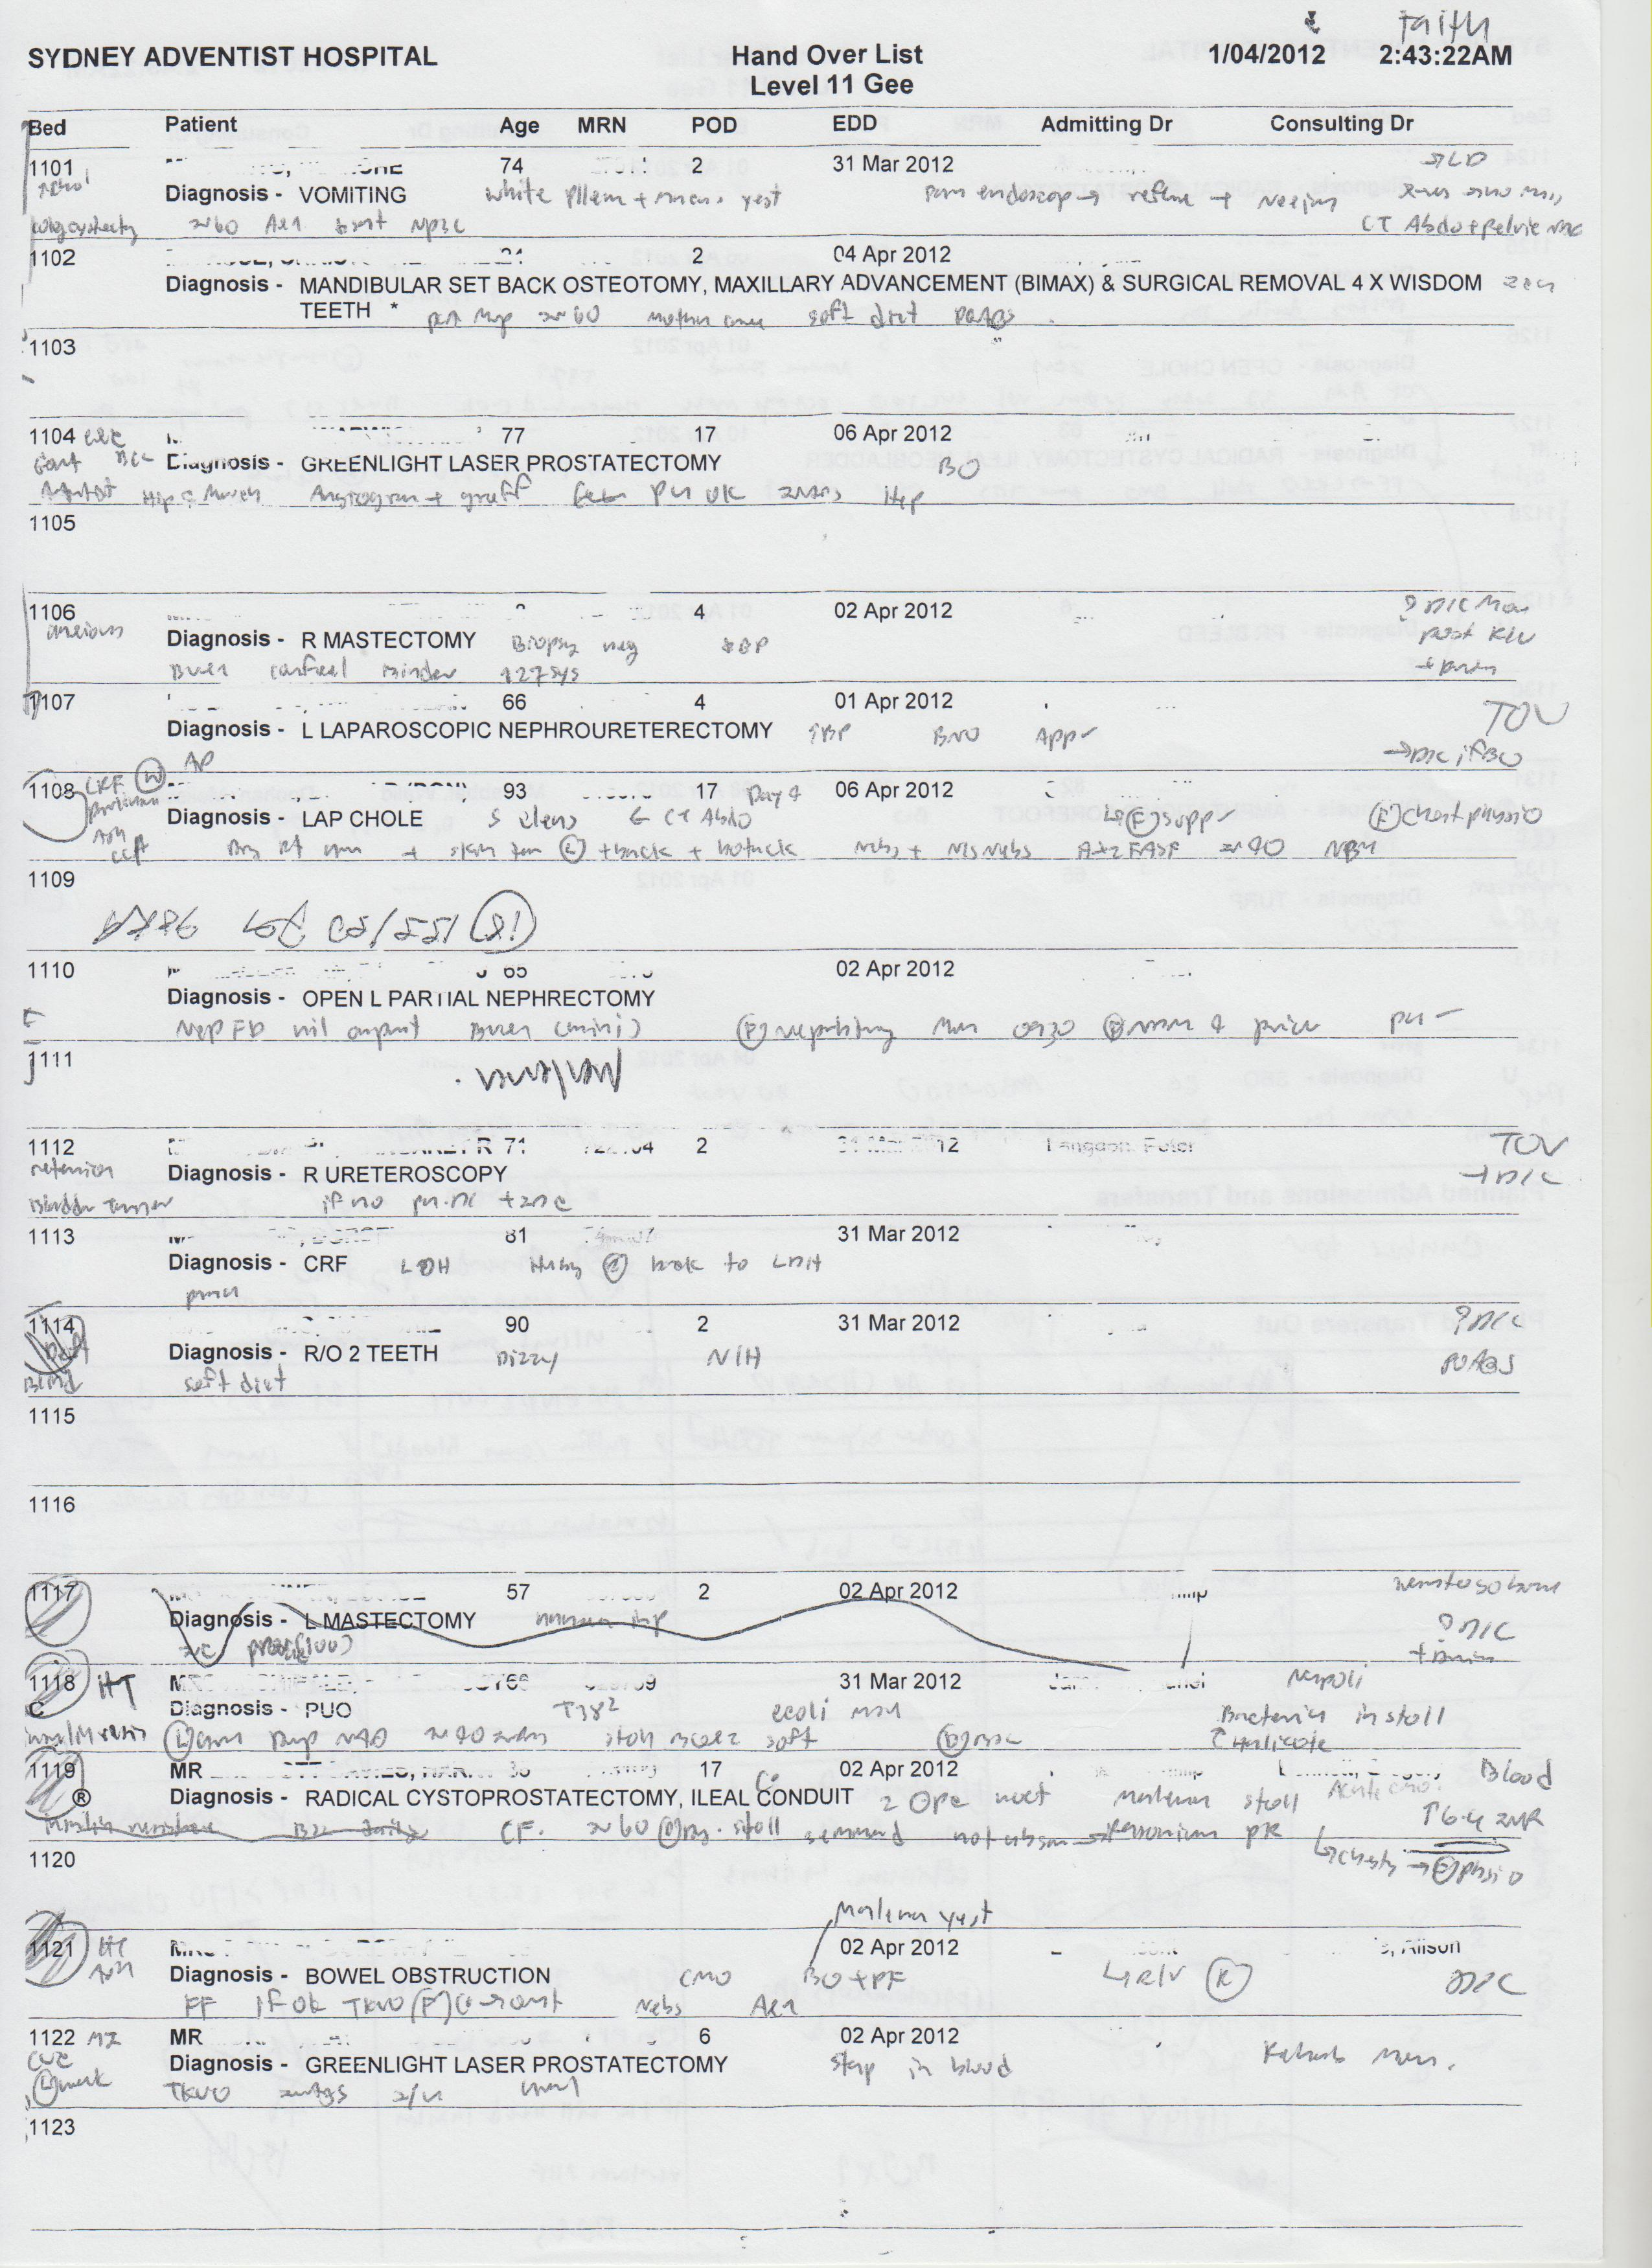
\includegraphics[scale=1.0, width=120mm]{Images/Patient-Handover-List-1}
				\caption{Patient Handover List - Front Page}
\end{figure} 

\begin{figure}[hp]
				\centering
				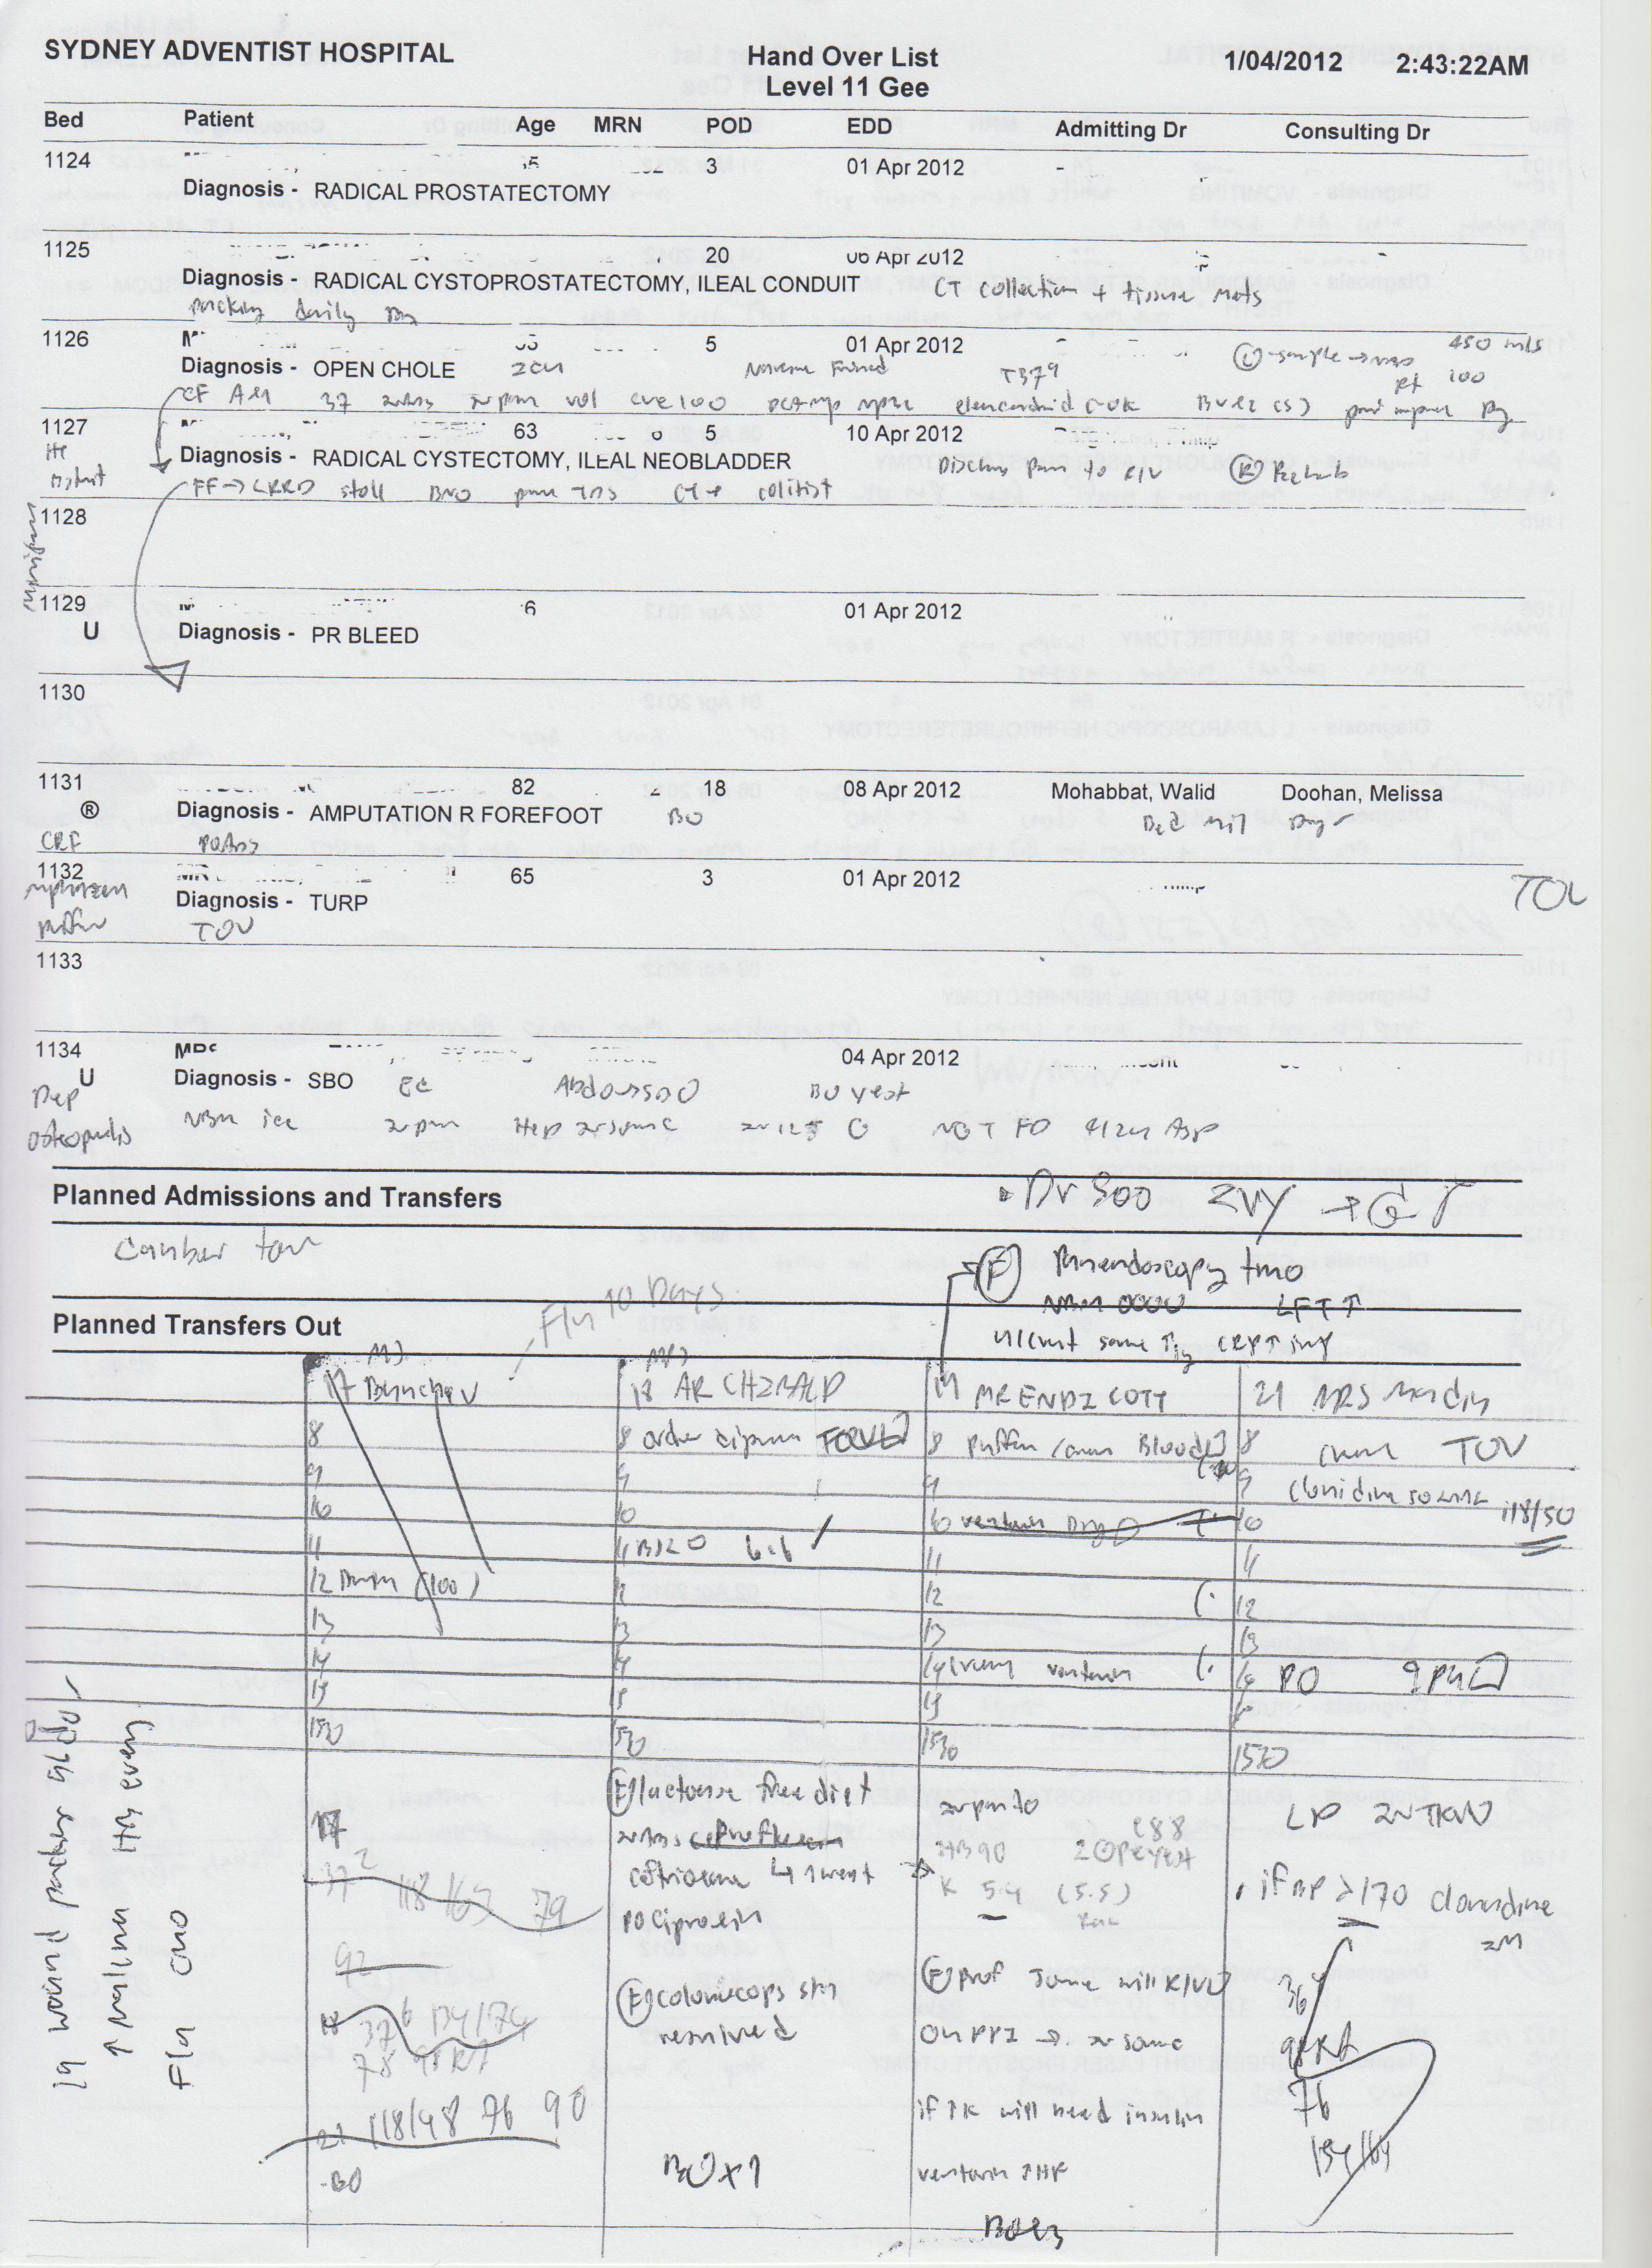
\includegraphics[scale=1.0, width=120mm]{Images/Patient-Handover-List-2}
				\caption{Patient Handover List - Back Page}
\end{figure}
 
\newpage
\subsection{Nursing Care Record Transformation}
\label{Nursing Care Record Transformation}

\begin{figure}[hp]
				\centering
				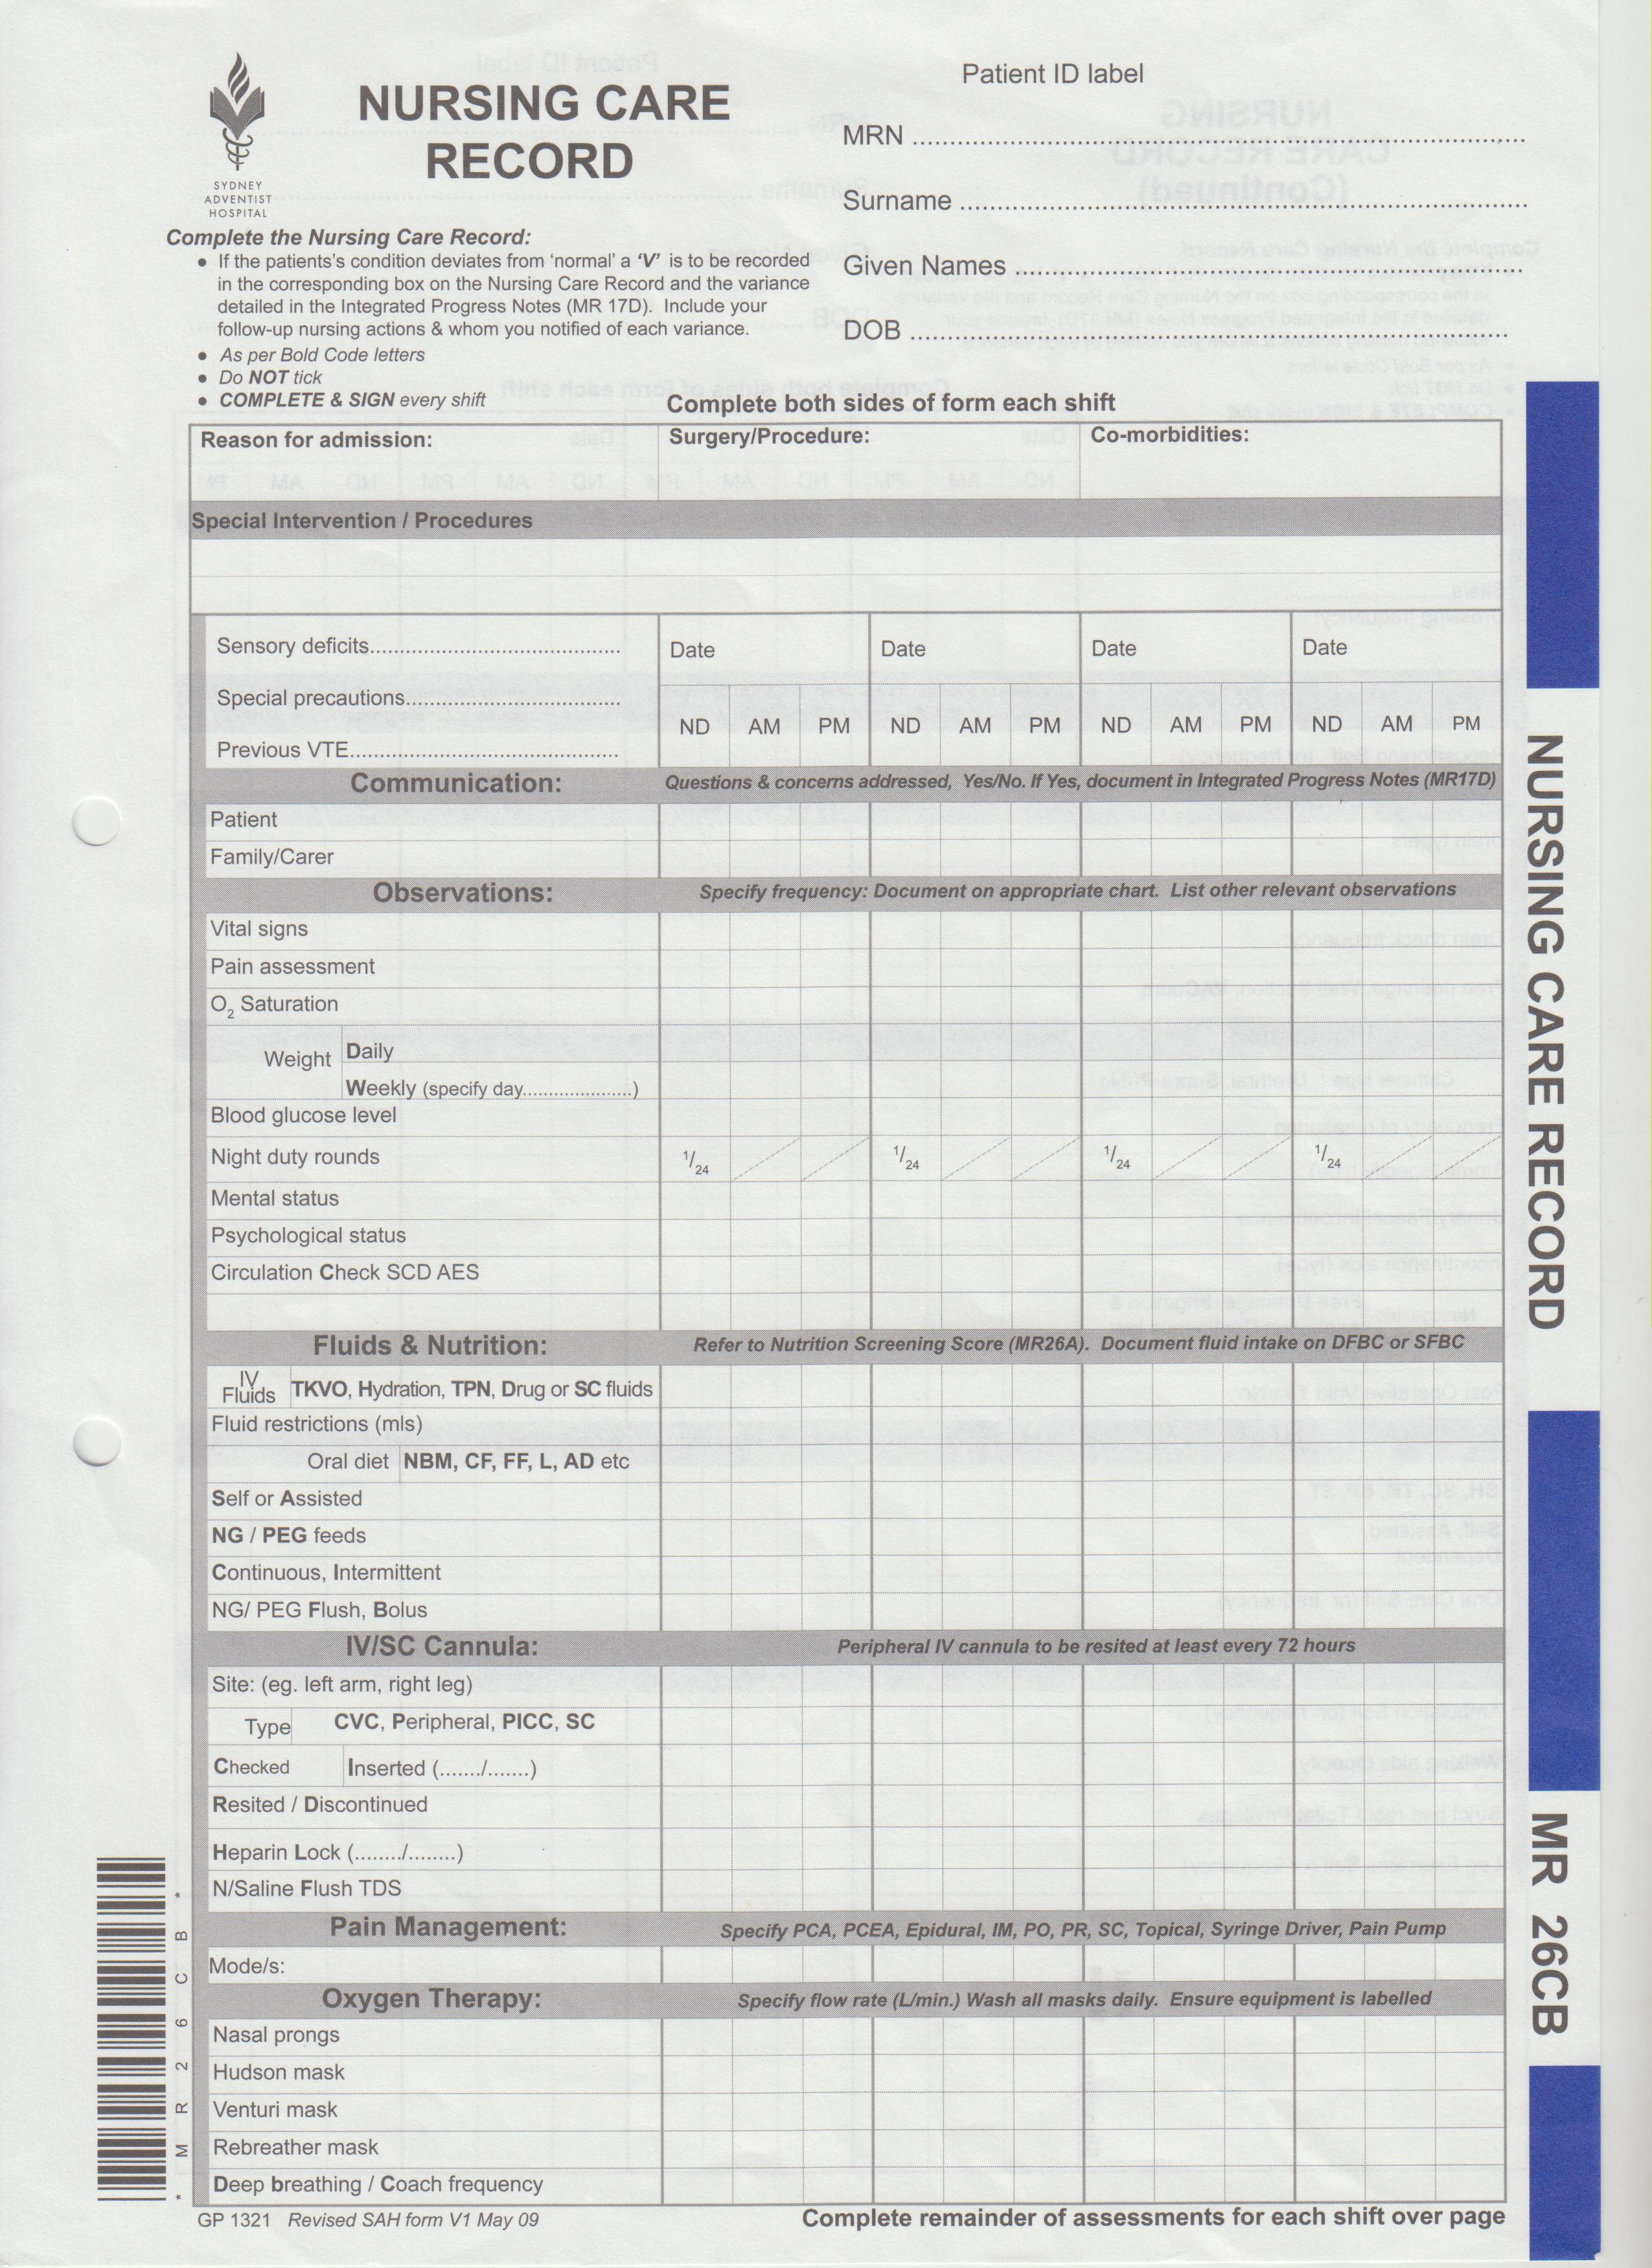
\includegraphics[scale=1.0, width=120mm]{Images/Nursing-Care-Record-Paper-1.jpg}
				\caption{Paper based Nursing Care Record - Front Page}
\end{figure} 
\newpage

\begin{figure}[hp]
				\centering
				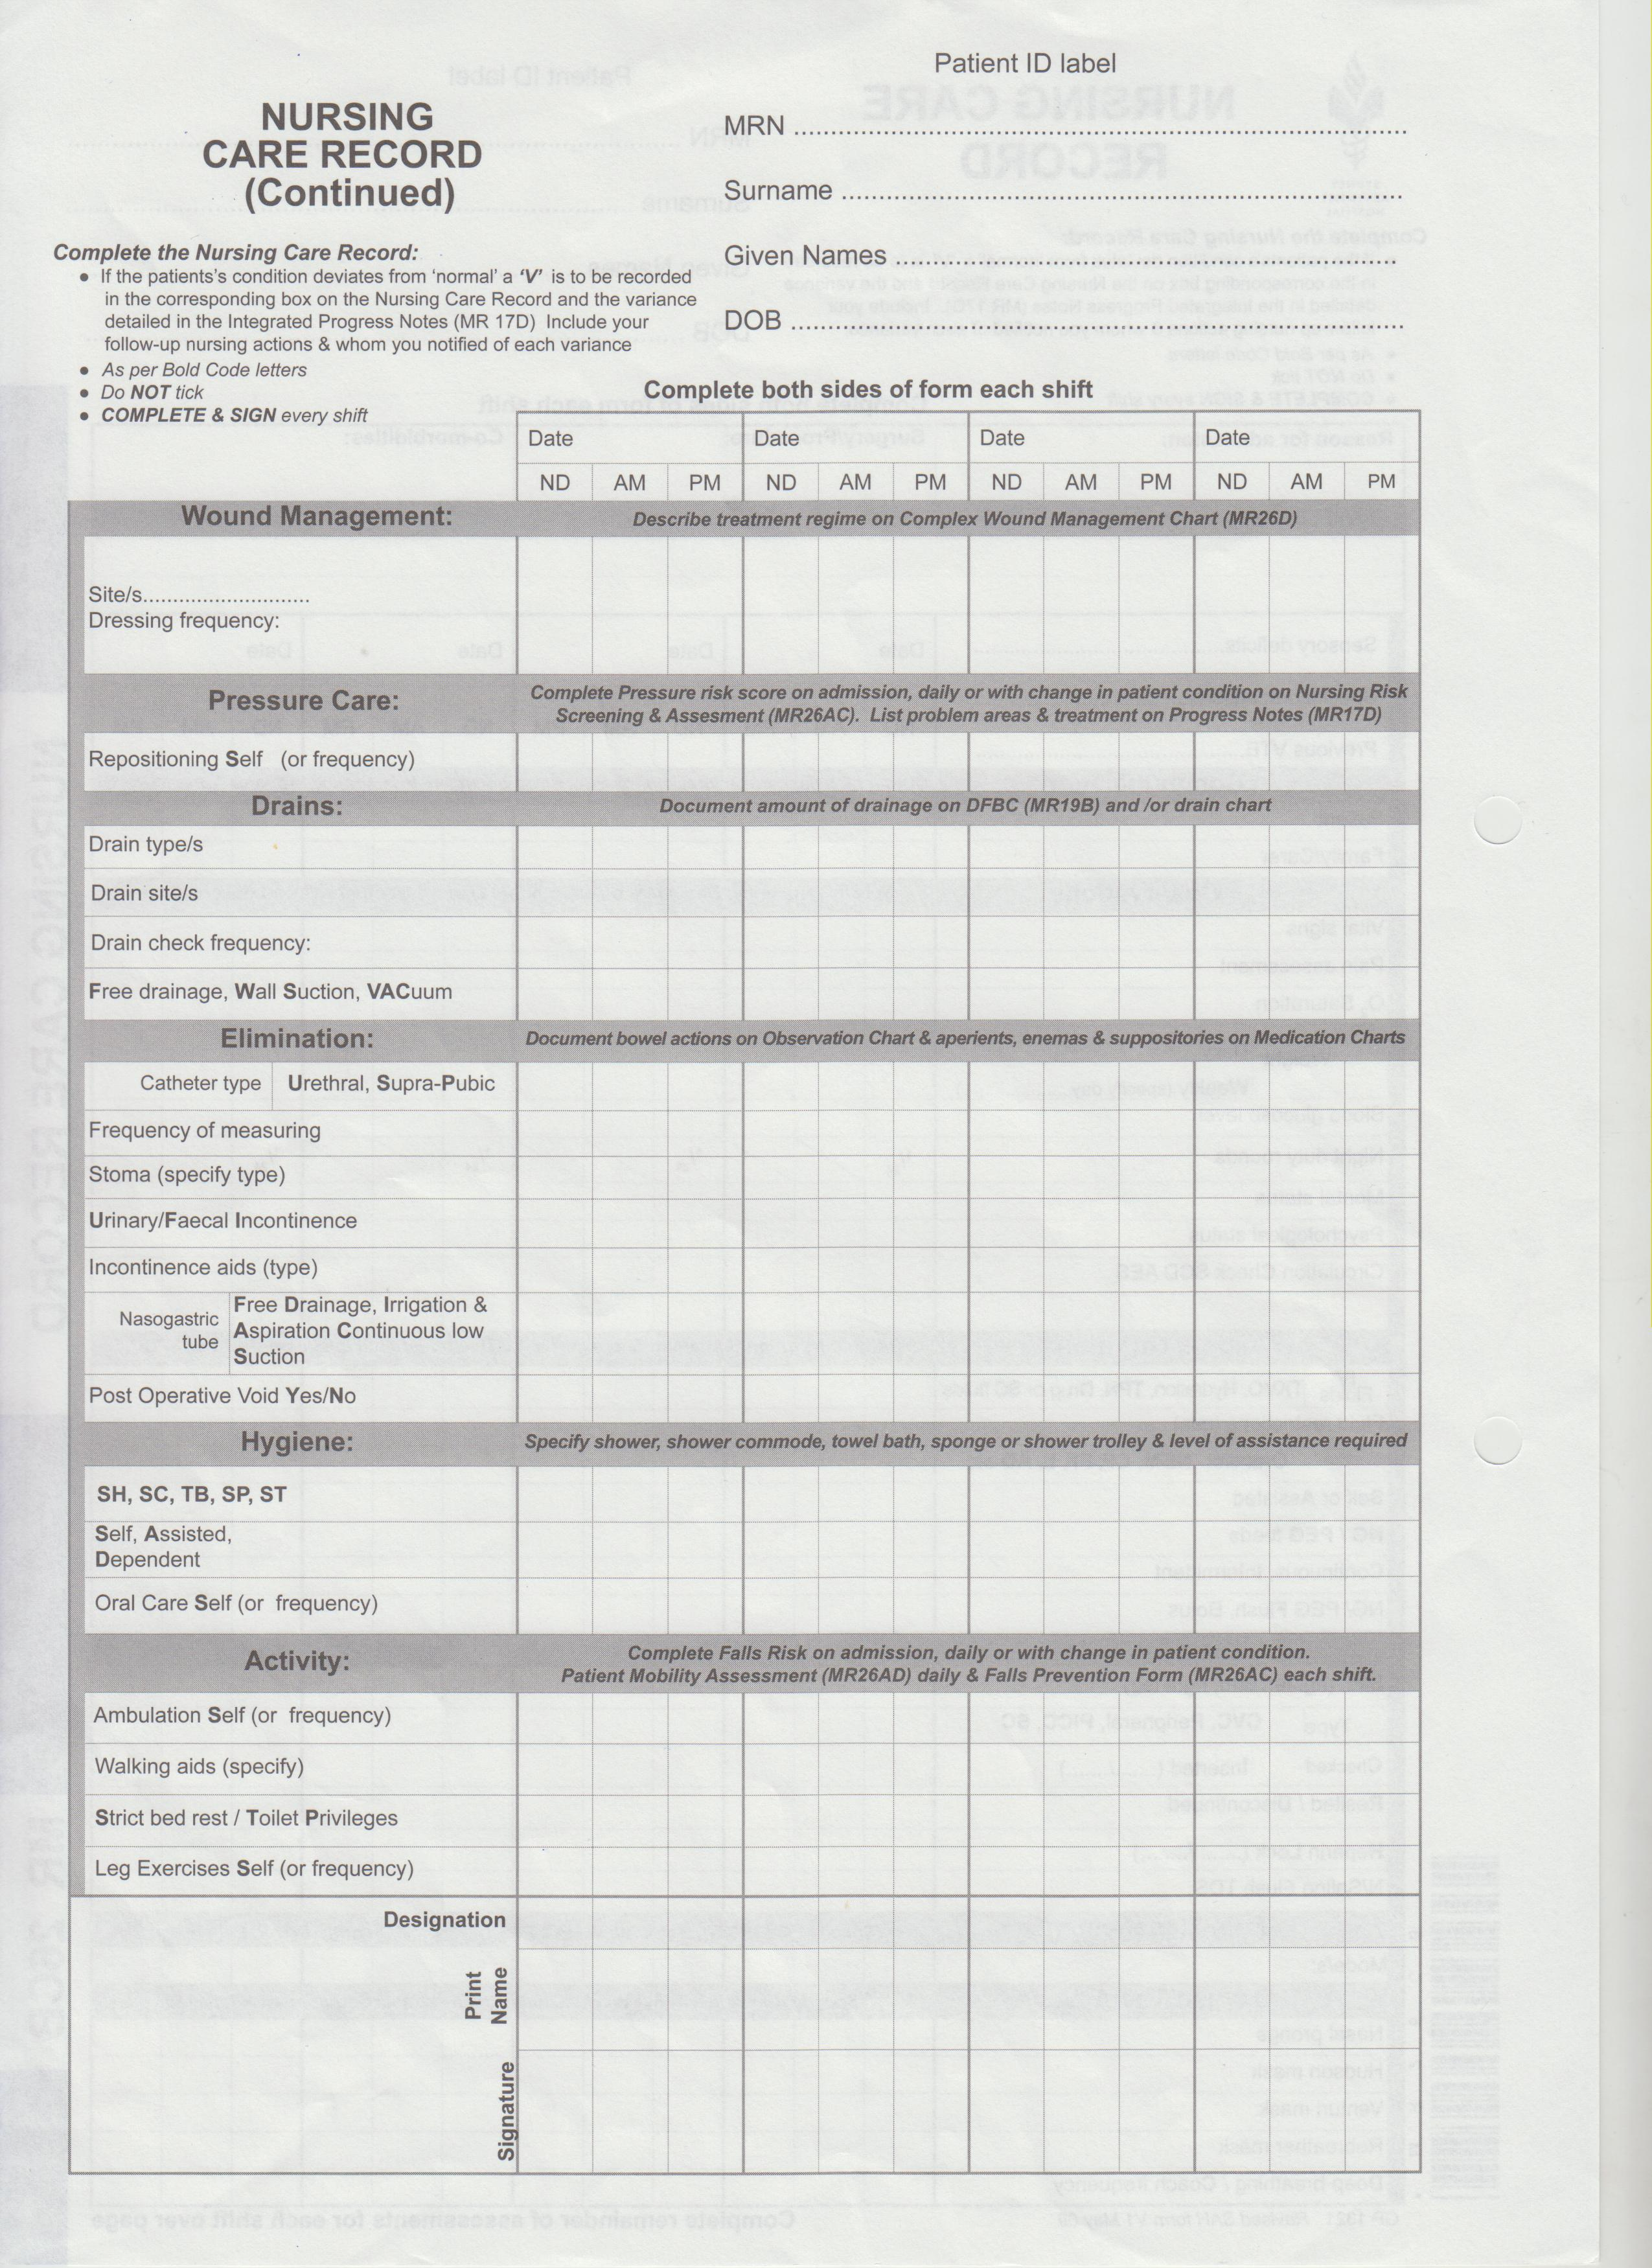
\includegraphics[scale=1.0, width=120mm]{Images/Nursing-Care-Record-Paper-2.jpg}
				\caption{Paper based Nursing Care Record - Back Page}
\end{figure} 

\newpage
\begin{figure}[hp]
				\centering
				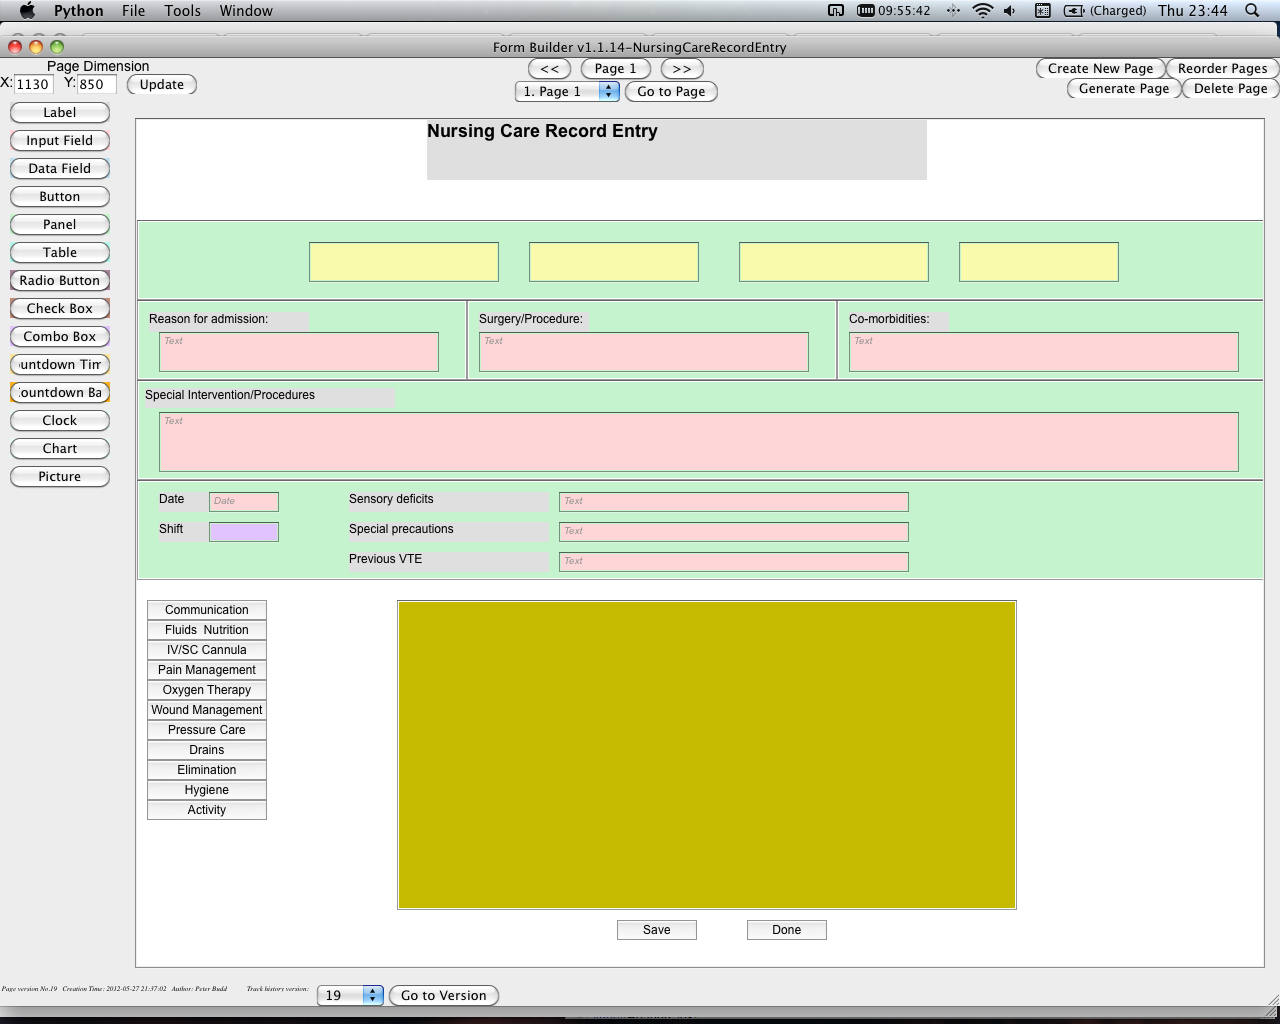
\includegraphics[angle=-90,scale=1.0, width=130mm]{Images/Nursing-Care-Record-Designer}
				\caption{Designer based Nursing Care Record}
				\label{Designer based Nursing Care Record}
\end{figure} 
\noindent The yellow section in the middle will be replaced by form content to which the buttons link. The user clicks on a button on the left and the relevant form section is displayed in the yellow section.

\newpage
\begin{figure}[hp]
				\centering
				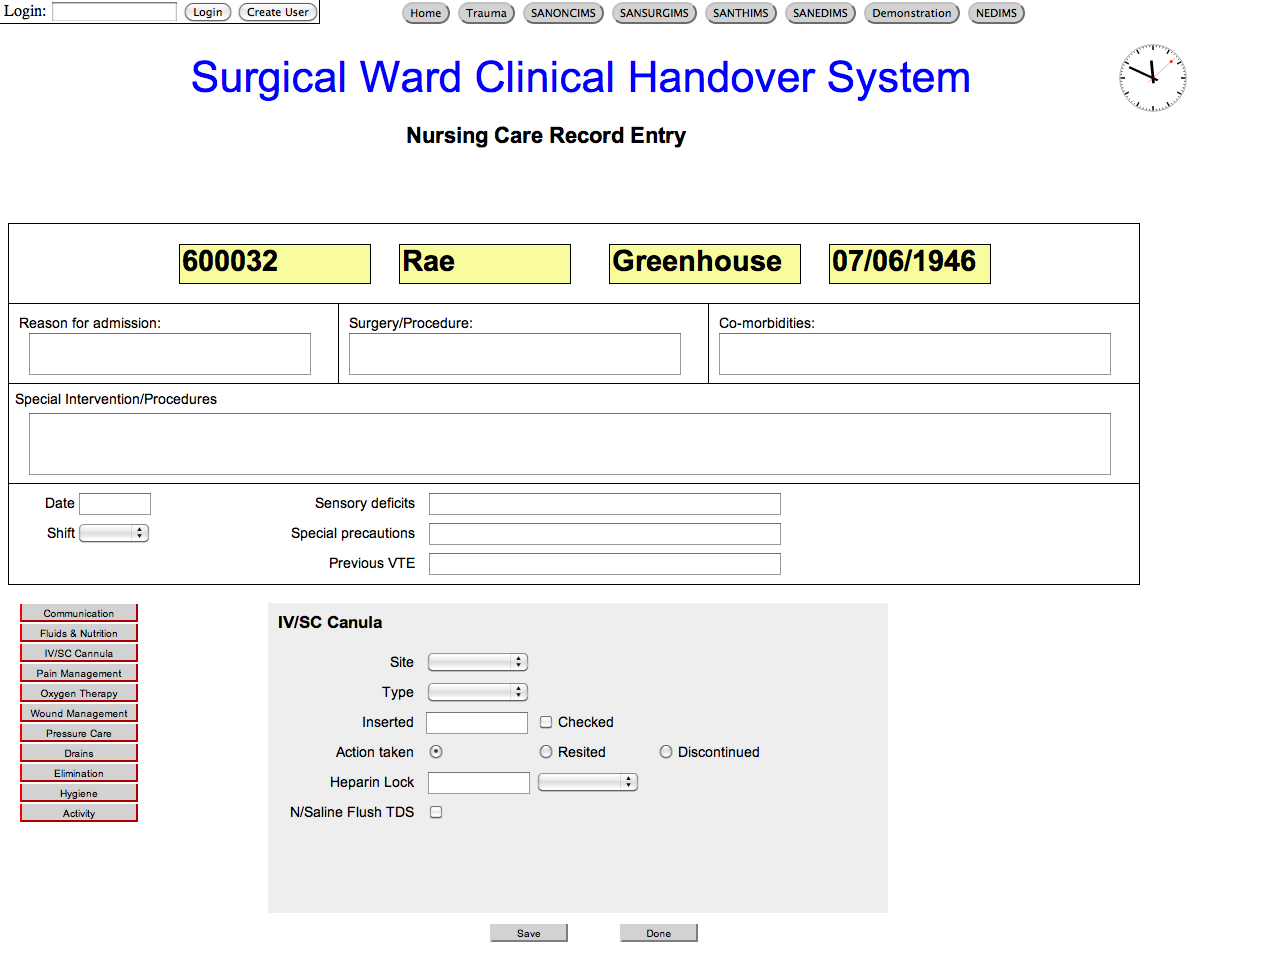
\includegraphics[angle=-90,scale=1.0, width=130mm]{Images/Nursing-Care-Record-Web}
				\caption{Web based Nursing Care Record}
\end{figure} 

\newpage
\subsection{Clinical Handover Questionnaire}
\label{Clinical Handover Questionnaire}

{\Large\textbf{Tasks}} \\
\indent\textbf{Level 6}
\begin{enumerate}
\item Go to the SANONCIMS system
\item View the Handover of Mauricio Patricia (Patient)
	\begin{enumerate}
	\item[1.] What medications is the patient on?
	\item[2.] What is the patient's O2 Saturation (SpO2)?
	\end{enumerate}
\end{enumerate} 

\indent\textbf{Level 11} 
\begin{enumerate}
\item Go to the SANSURGIMS system
\item View the Handover of Hogans Zelma (Patient)
	\begin{enumerate}
	\item[1.] What medications is the patient on?
	\item[2.] Does the patient require assistance?
	\end{enumerate}
\end{enumerate} 

\noindent{\Large\textbf{Questions}}
\begin{enumerate}
\item Is it too much information?
	\begin{enumerate}
	\item[1.] too much information
	\item[2.] alot of information
	\item[3.] contains unneeded information
	\item[4.] contains the right information but needs improvement
	\item[5.] just the right amount of information
	\end{enumerate}
\item Is it easy to find information?
	\begin{enumerate}
	\item[1.] cannot find information
	\item[2.] very difficult to find information
	\item[3.] can find information but take a long time
	\item[4.] can find information
	\item[5.] very easy to find information
	\end{enumerate}

\newpage
\item Is the information logical to you?
	\begin{enumerate}
	\item[1.] very unordered
	\item[2.] very cluttered
	\item[3.] somewhat cluttered
	\item[4.] mostly ordered
	\item[5.] very ordered
	\end{enumerate}
\item Are the colours informative?
	\begin{enumerate}
	\item[1.] distracts from information
	\item[2.] does not give any extra information
	\item[3.] highlighting useful
	\item[4.] adds extra information
	\item[5.] highlights vital information
	\end{enumerate}
\item Does this form make handover more efficient for you?
	\begin{enumerate}
	\item[1.] does not help at all
	\item[2.] as efficient as current handover process
	\item[3.] not sure
	\item[4.] improves efficiency
	\item[5.] greatly improves efficiency
	\end{enumerate}
\item Is it easy to navigate?
	\begin{enumerate}
	\item[1.] unable to navigate
	\item[2.] confusing to navigate
	\item[3.] navigate with problems
	\item[4.] able to navigate
	\item[5.] very intuitive
	\end{enumerate}
\end{enumerate}

\newpage
\subsection{SANSURGIMS Data Flow}
\label{SANSURGIMS Data Flow}

Data flow within SANSURGIMS is quite simple. The data entry forms are all used to supply the handover form with data. The only forms in SANSURGIMS that do not feed information into the handover form are the General Patient Information Form, the Tracking List Form and various table forms. These tables forms are used merely for listing all instances of the data entry forms. They do not contribute any data or information themselves. Figure \ref{Data Flow} shows how all data flows from the data entry forms to the handover.

\begin{figure}[hp]
				\centering
				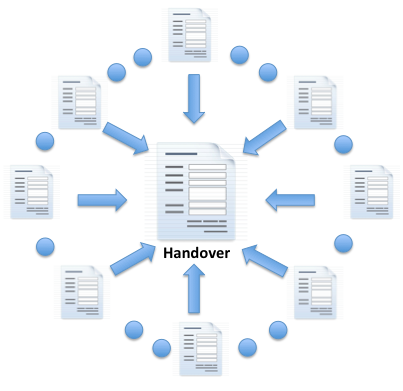
\includegraphics[scale=1.0, width=123mm]{Images/DataFlow}
				\caption{Data Flow within SANSURGIMS}
				\label{Data Flow}
\end{figure} 

\newpage
\subsection{SANSURGIMS Work Flow}
\label{SANSURGIMS Work Flow}
The following sections outline workflows within SANSURGIMS based on forms.

\subsubsection{Handover}
The user starts on the ward tracking list and proceeds to select a patient handover by clicking on the ``Handover" button in the row that corresponds to that patient. The user will be shown the handover form and if the user requires, he or she can obtain more information by navigating to specific clinical forms through the button menu at the bottom of the page. The user returns to the handover form by clicking on the ``Done" button on the clinical form page. When the user has all of the information he or she needs, they return to the tracking list via the ``Tracking List" button.

\begin{figure}[hp]
				\centering
				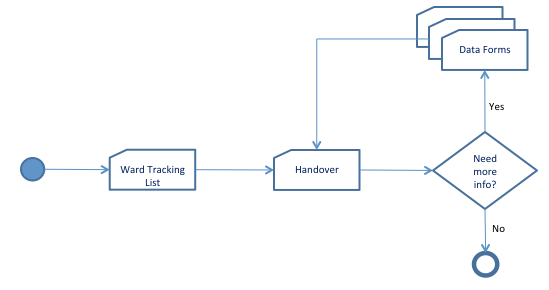
\includegraphics[scale=1.0, width=123mm]{Images/Handover-Workflow}
				\caption{Handover Workflow within SANSURGIMS}
\end{figure}

\newpage
\subsubsection{General Patient Information}
The user starts on the ward tracking list and proceeds to select a patient's general information by clicking on the ``i" button in the row that corresponds to that patient. The user will be shown the patient's general information and is able to edit this information to reflect updates to the patient. Once finished, the user returns to the ward tracking list by clicking on the ``Done" button.

\begin{figure}[hp]
				\centering
				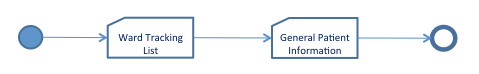
\includegraphics[scale=1.0, width=123mm]{Images/General-Patient-Information}
				\caption{General Patient Information Workflow within SANSURGIMS}
\end{figure}

\subsubsection{Data Entry}
The user starts on the ward tracking list and proceeds to select a patient's handover by clicking on the ``Handover" button in the row that corresponds to that patient. The user will be shown the handover form and can find buttons to various clinical forms at the bottom of the form. By clicking on the button corresponding to the form the user requires, he or she will be transferred to that form in order to enter information pertaining to the patient. Once the user is finished entering data, the user saves and return to the handover form by clicking on the ``Done" button. The user can proceed to another clinical form or finish his or her work by clicking on the ``Tracking List" button to return to the ward tracking list.

\begin{figure}[hp]
				\centering
				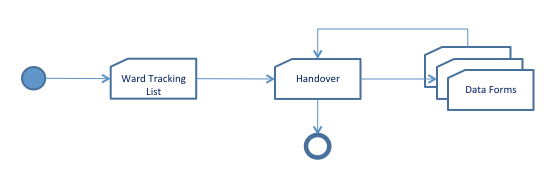
\includegraphics[scale=1.0, width=123mm]{Images/Data-Entry}
				\caption{Data Entry Workflow within SANSURGIMS}
\end{figure}

\newpage
\subsection{SANSURGIMS Screenshots}

\subsubsection{Patient Tracking List}
\label{Patient Tracking List}
\begin{figure}[hp]
				\centering
				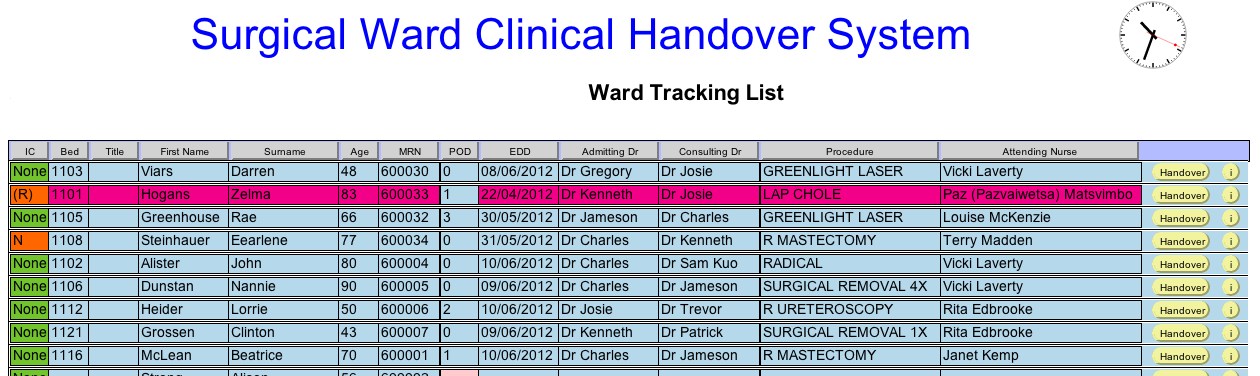
\includegraphics[scale=1.0, width=123mm]{Images/iCIMS-Tracking-List-Cropped}
				\caption{Patient Tracking List}
\end{figure} 

\vspace{-10mm}
\subsubsection{Non-complex Patient Handover}
\label{Very Uncomplex Patient}

\begin{figure}[hp]
				\centering
				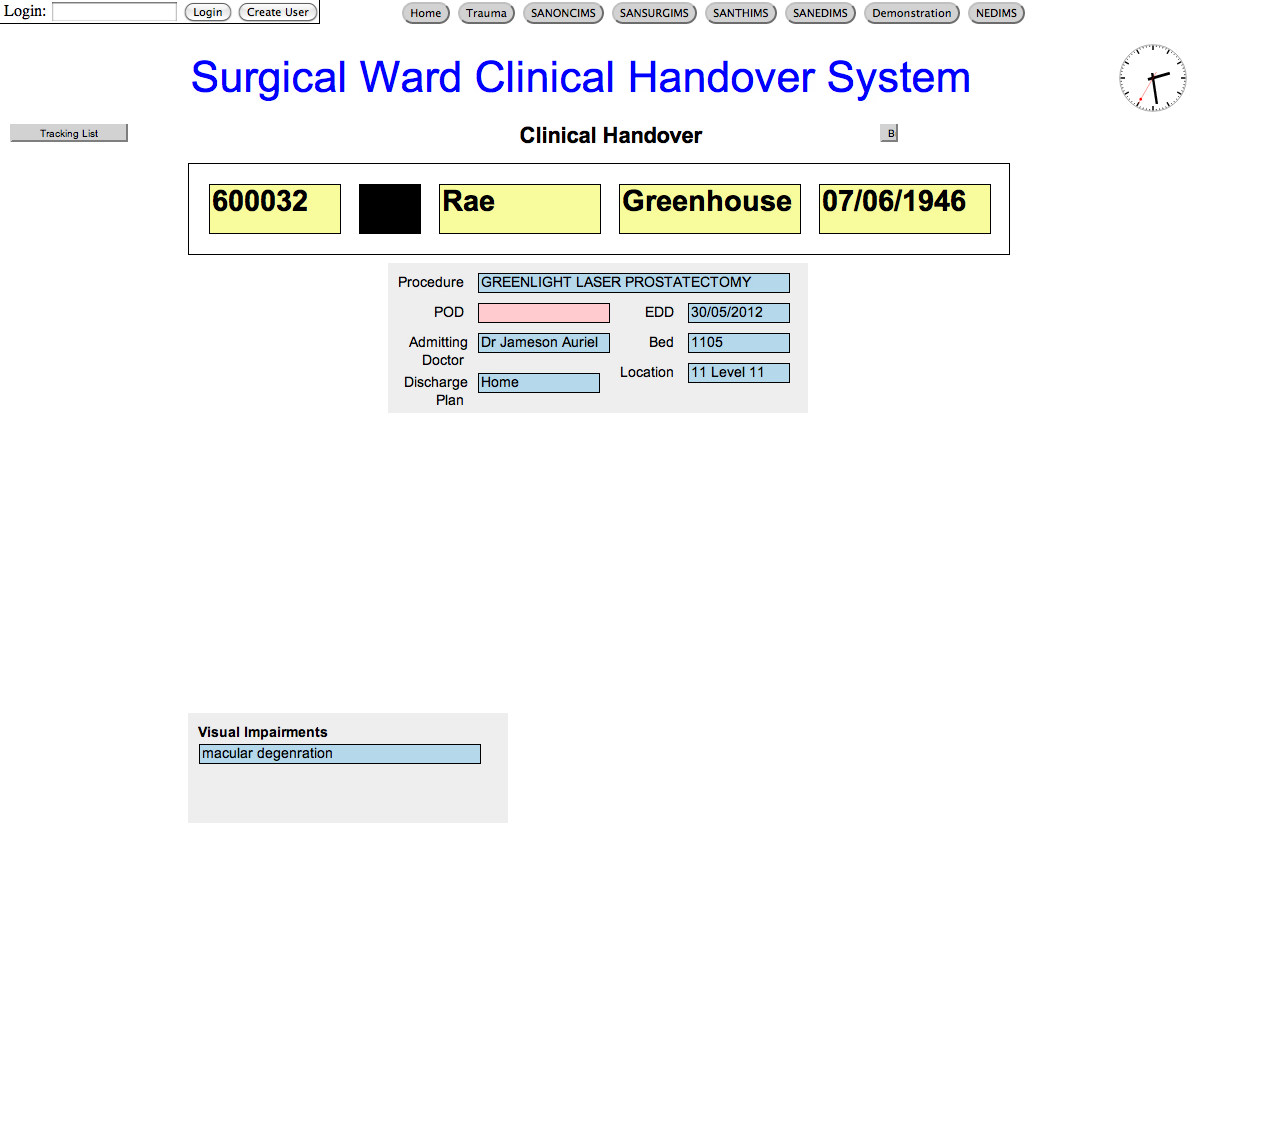
\includegraphics[scale=1.0, width=123mm]{Images/iCIMS-Very-Uncomplex-Patient}
				\caption{Handover - Non-complex Patient}
\end{figure} 

\newpage
\subsubsection{Somewhat Complex Patient Hanover}
\label{Somewhat Complex Patient}

\begin{figure}[hp]
				\centering
				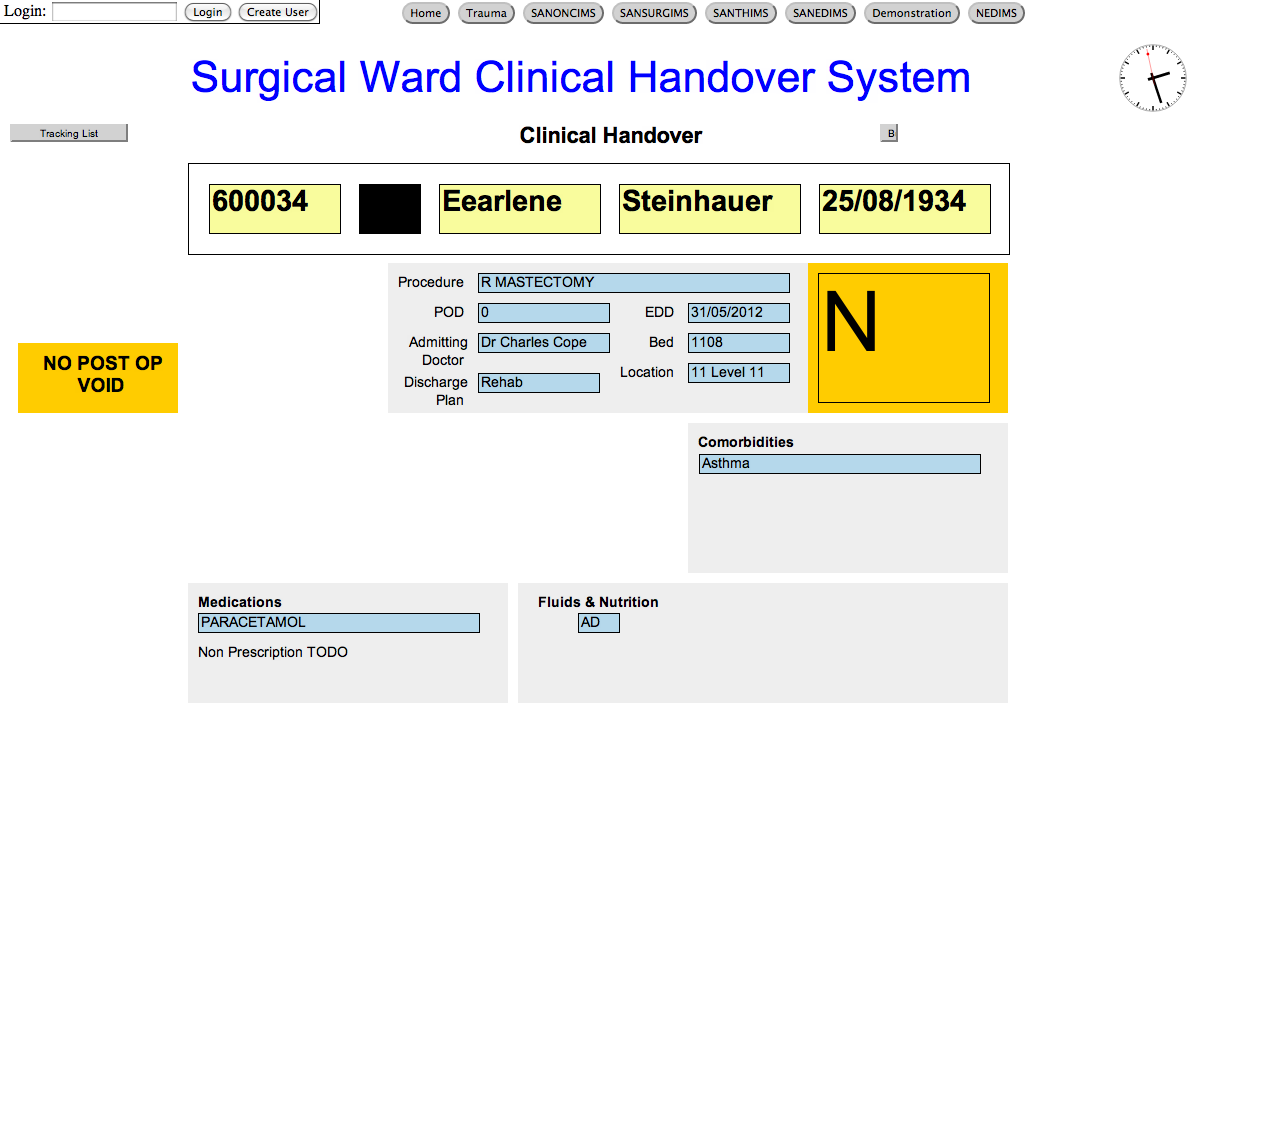
\includegraphics[scale=1.0, width=180mm]{Images/iCIMS-Medium-Patient}
				\caption{Handover - Somewhat Complex Patient}
\end{figure} 

\newpage
\subsubsection{Very Complex Patient Handover}
\label{Very Complex Patient}

\begin{figure}[hp]
				\centering
				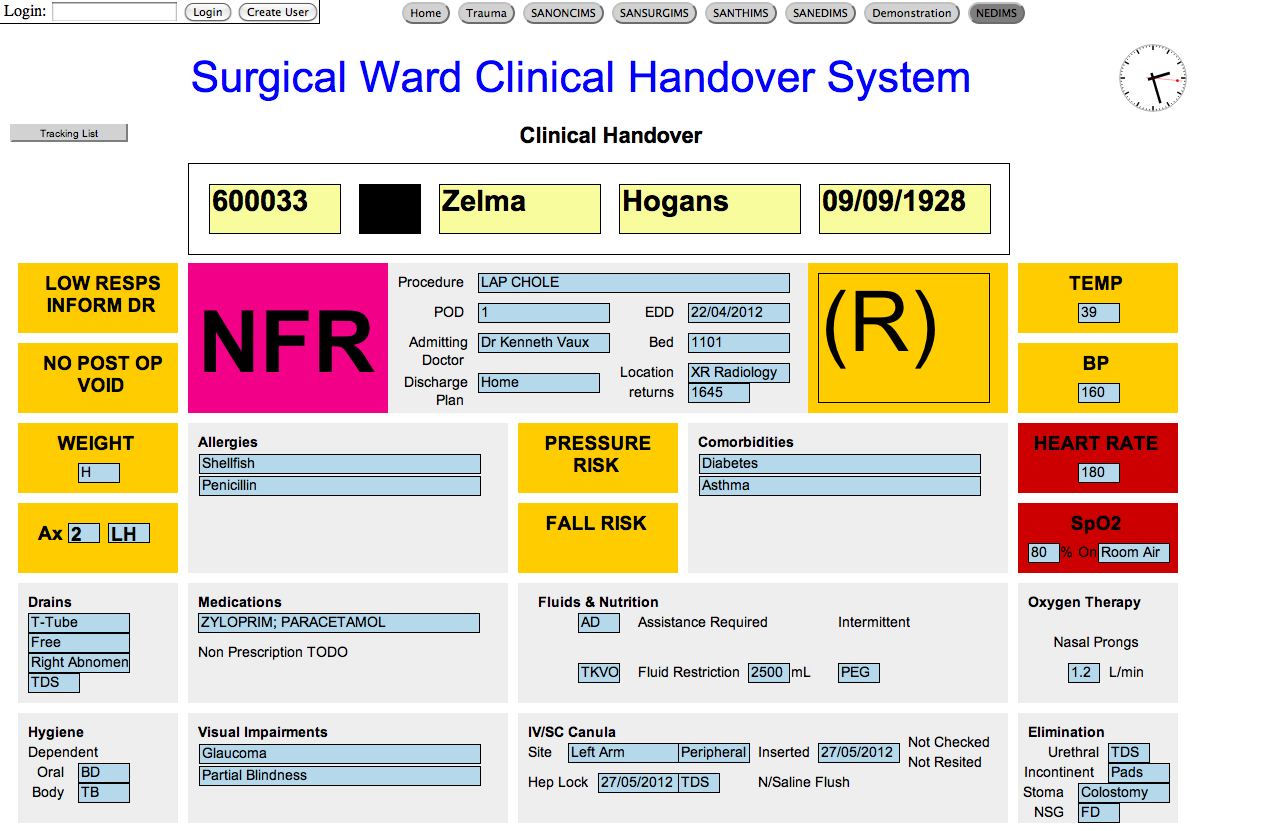
\includegraphics[scale=1.0, width=180mm]{Images/iCIMS-Complex-Patient}
				\caption{Handover - Very Complex Patient}
\end{figure} 

\newpage
\subsubsection{General Patient Information Form}
\label{General Patient Information}

\begin{figure}[hp]
				\centering
				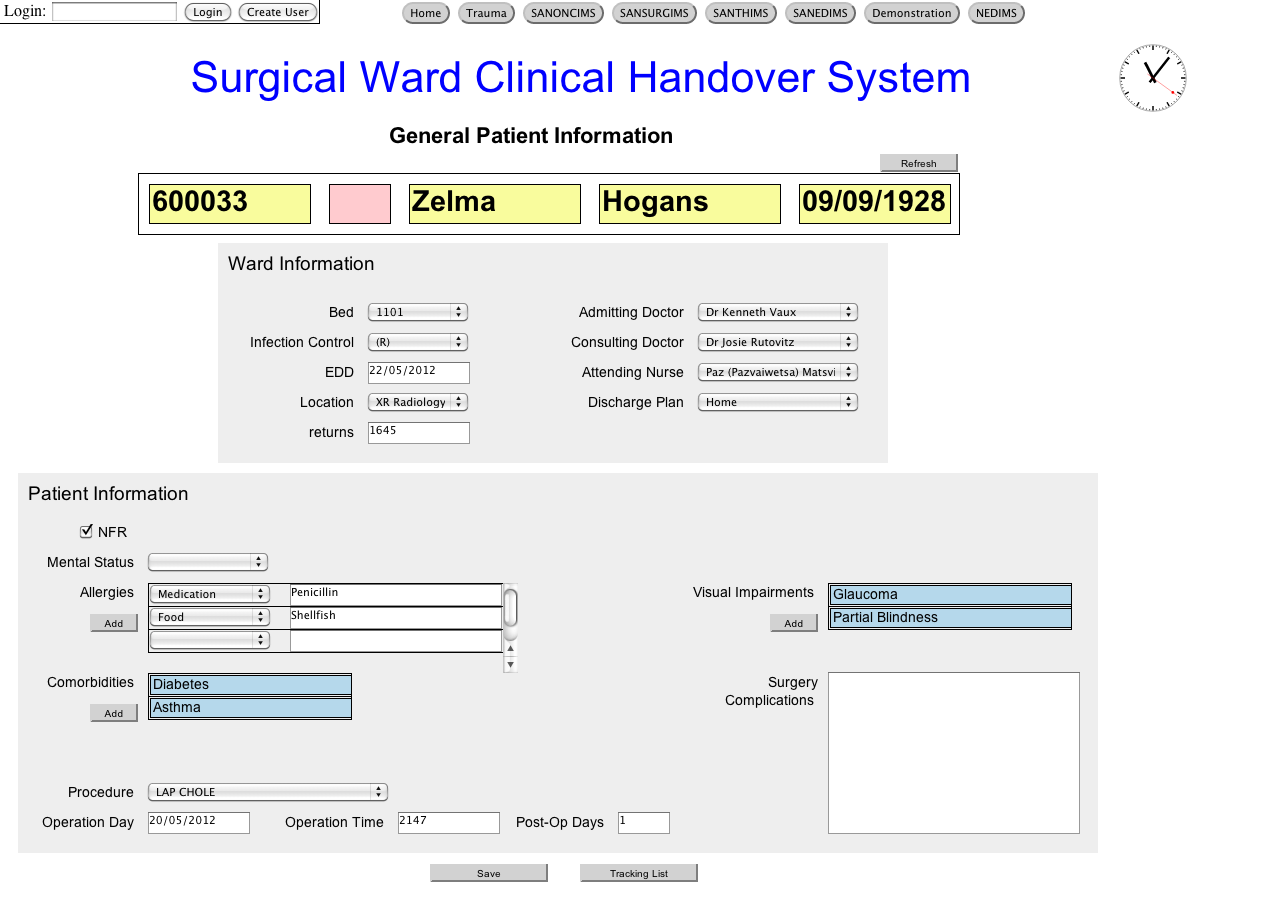
\includegraphics[scale=1.0, width=180mm]{Images/iCIMS-General-Patient-Information}
				\caption{General Patient Information Form}
\end{figure} 

\newpage
\subsubsection{Pain and Symptom Assessment Entry Form}
\label{Pain and Symptom Assessment Entry Form}
\begin{figure}[hp]
				\centering
				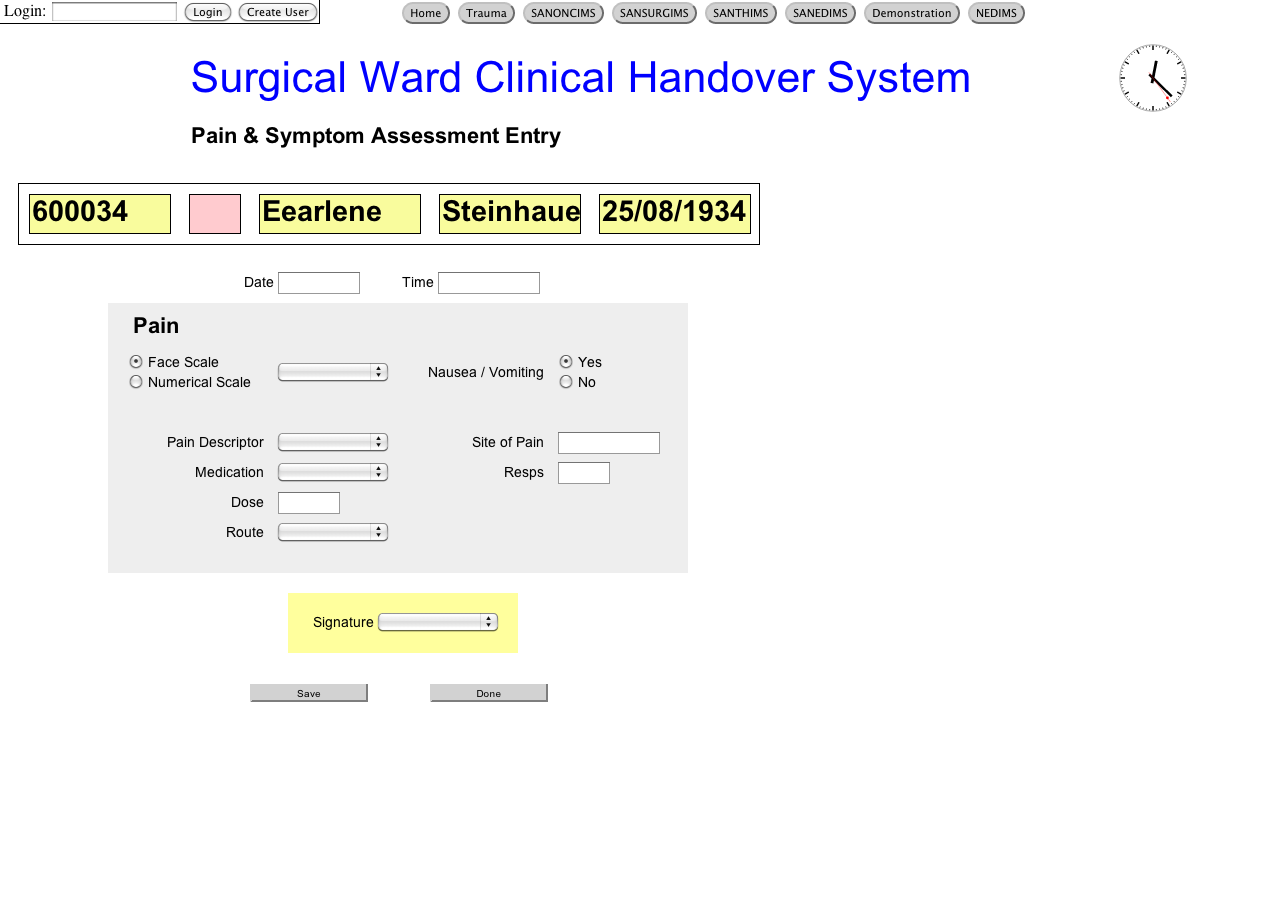
\includegraphics[scale=1.0, width=123mm]{Images/iCIMS-PainSymptomAssessment}
				\caption{Pain and Symptom Assessment Entry Form}
\end{figure} 

\newpage
\subsubsection{Pain and Symptom Assessment Table Form}
\label{Pain and Symptom Assessment Table Form}

\begin{figure}[hp]
				\centering
				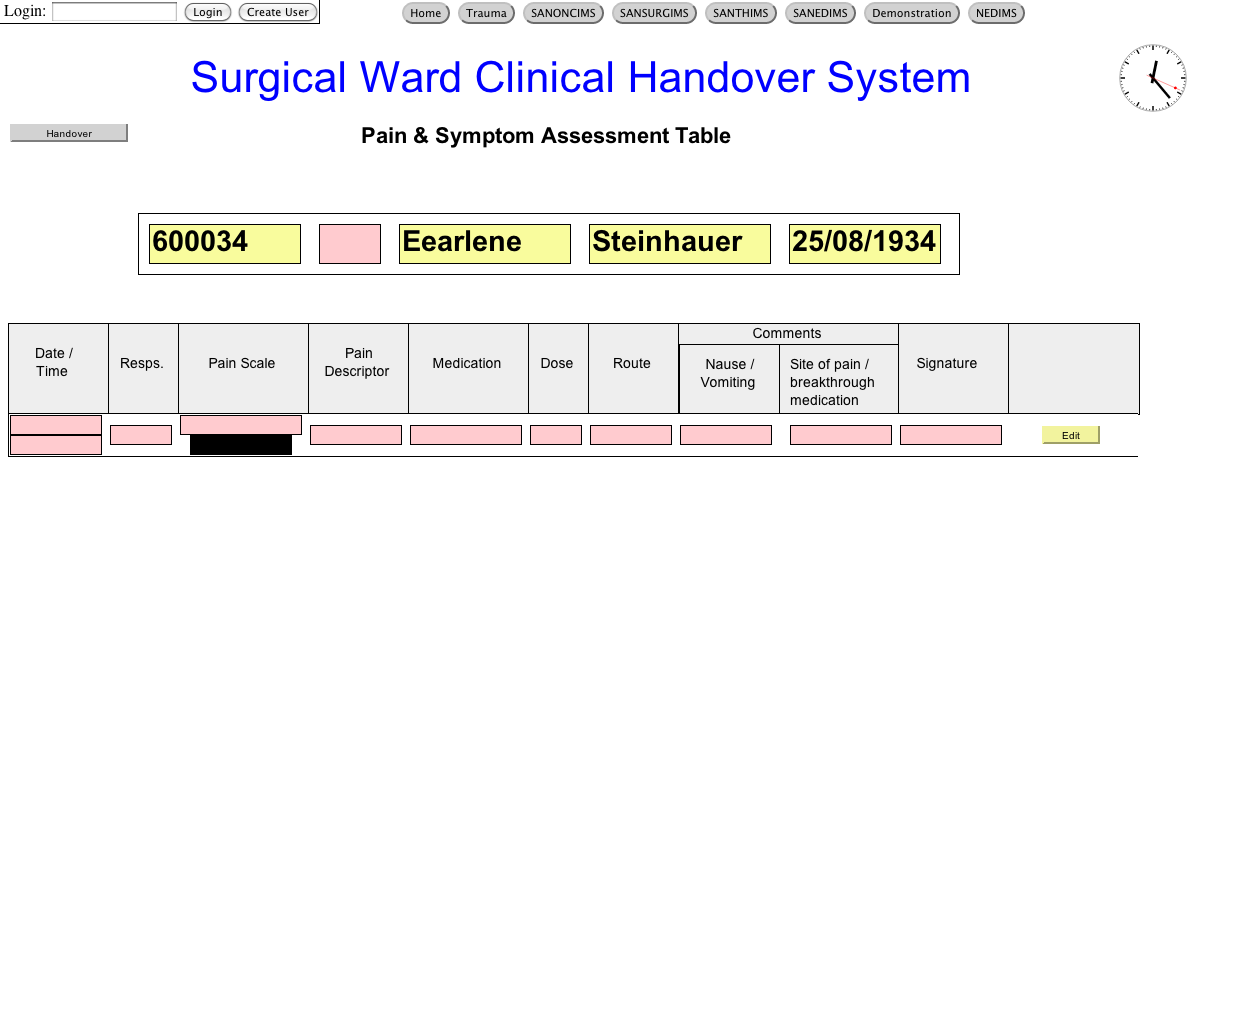
\includegraphics[scale=1.0, width=180mm]{Images/iCIMS-PainSymptomAssesmentTable}
				\caption{Pain and Symptom Assessment Table Form}
\end{figure} 

\newpage
\subsubsection{Nursing Care Record Entry Form}
\label{Nursing Care Record Entry Form}

\begin{figure}[hp]
				\centering
				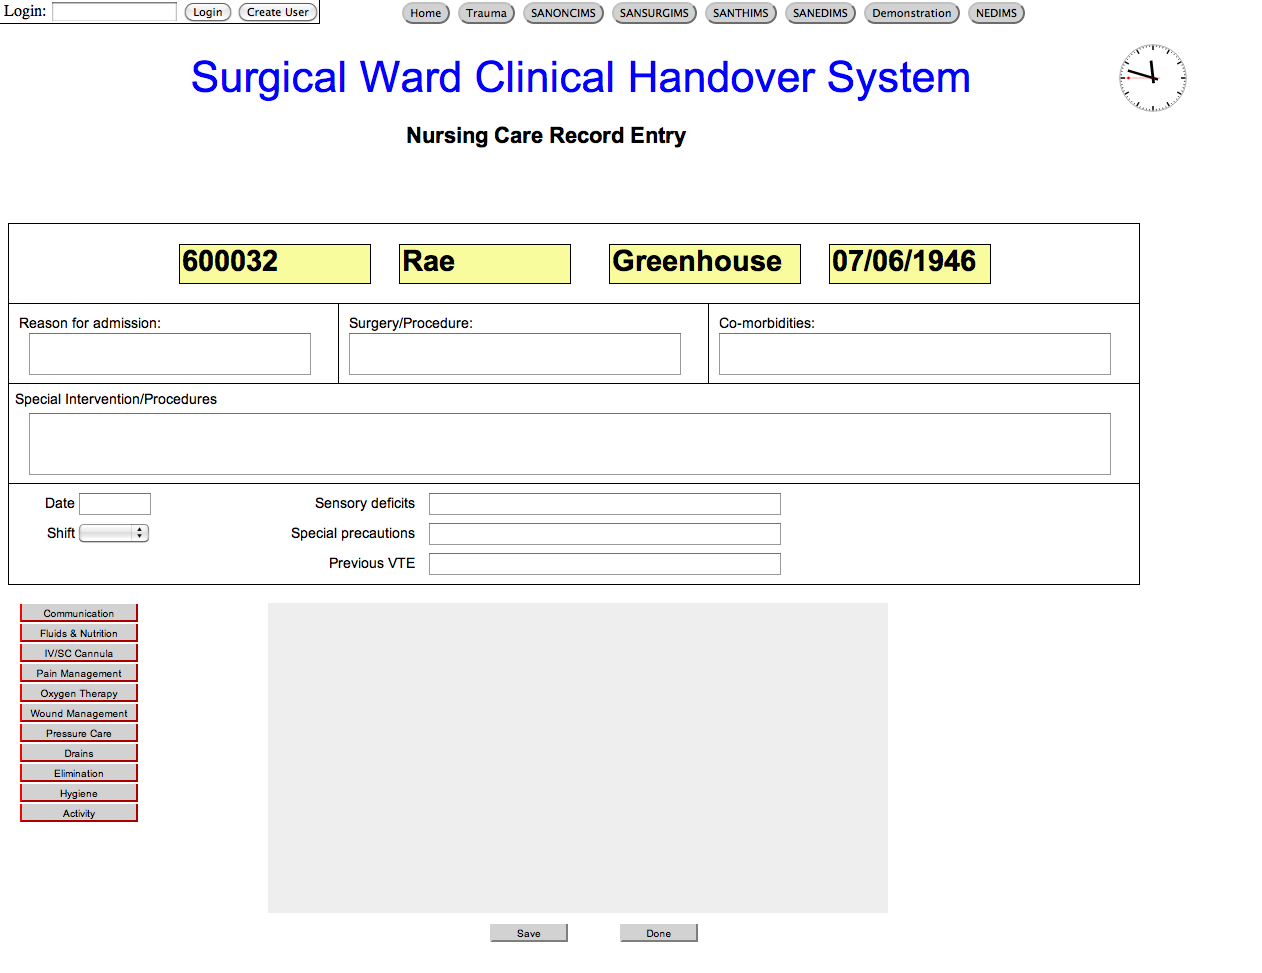
\includegraphics[scale=1.0, width=180mm]{Images/iCIMS-NCREmpty}
				\caption{Nursing Care Record Entry Form - Start Page}
\end{figure} 

\newpage
\begin{figure}[hp]
				\centering
				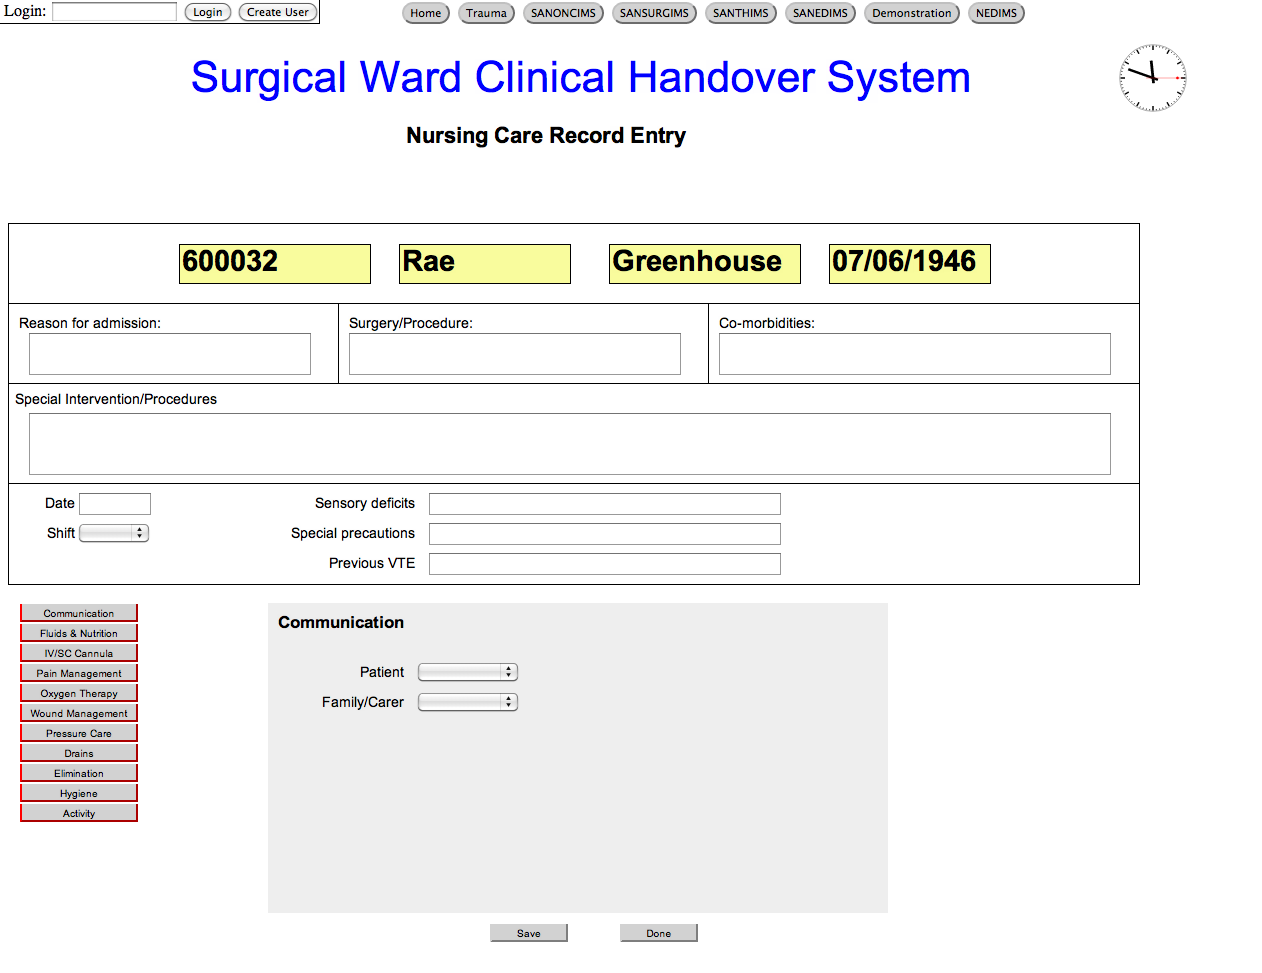
\includegraphics[scale=1.0, width=180mm]{Images/iCIMS-NCRCommunication}
				\caption{Nursing Care Record Entry Form - Communication}
\end{figure} 

\newpage
\begin{figure}[hp]
				\centering
				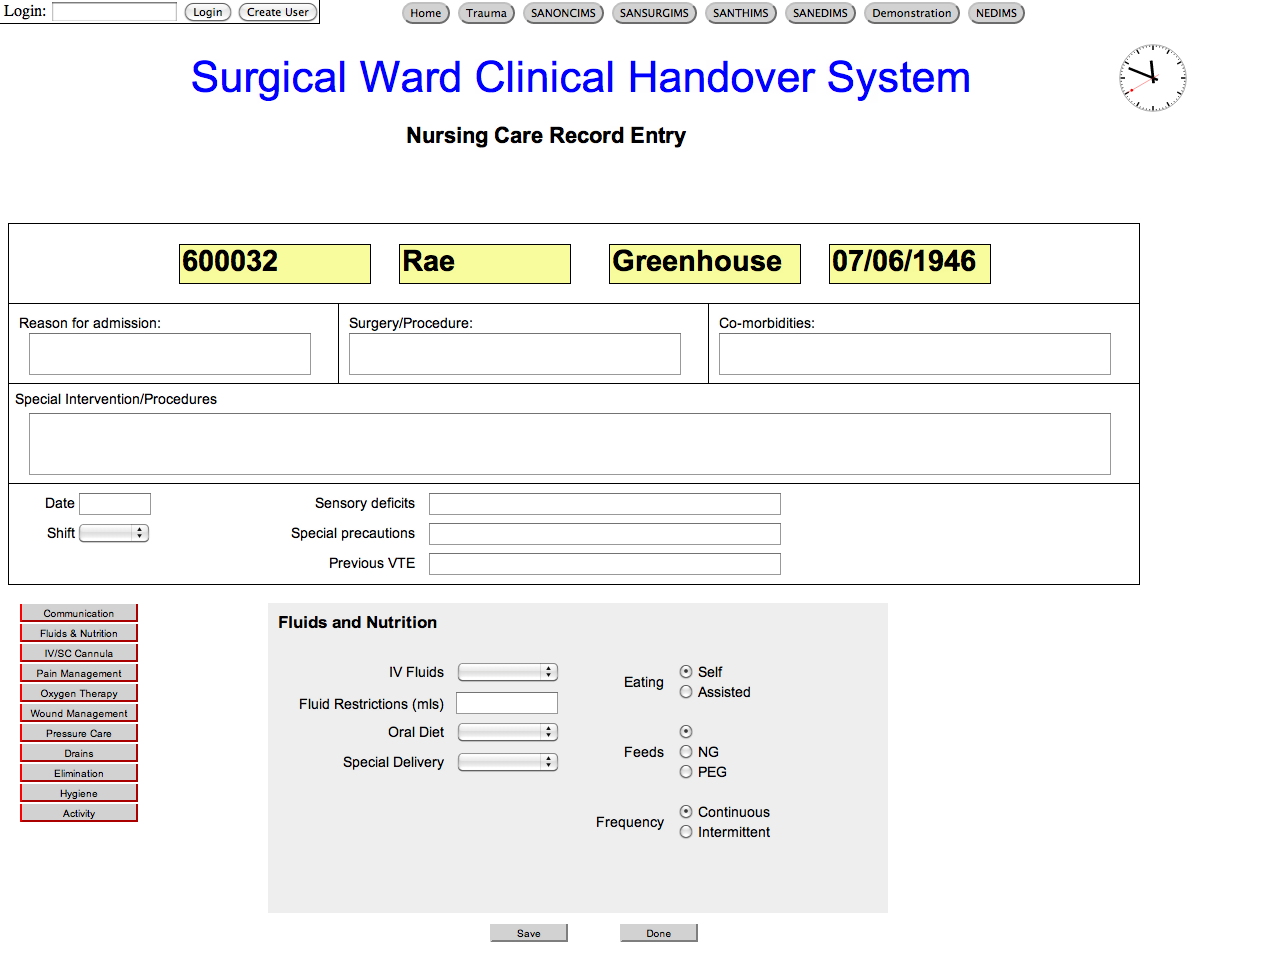
\includegraphics[scale=1.0, width=180mm]{Images/iCIMS-NCRFluidsNutrition}
				\caption{Nursing Care Record Entry Form - Fluids and Nutrition}
\end{figure} 

\newpage
\begin{figure}[hp]
				\centering
				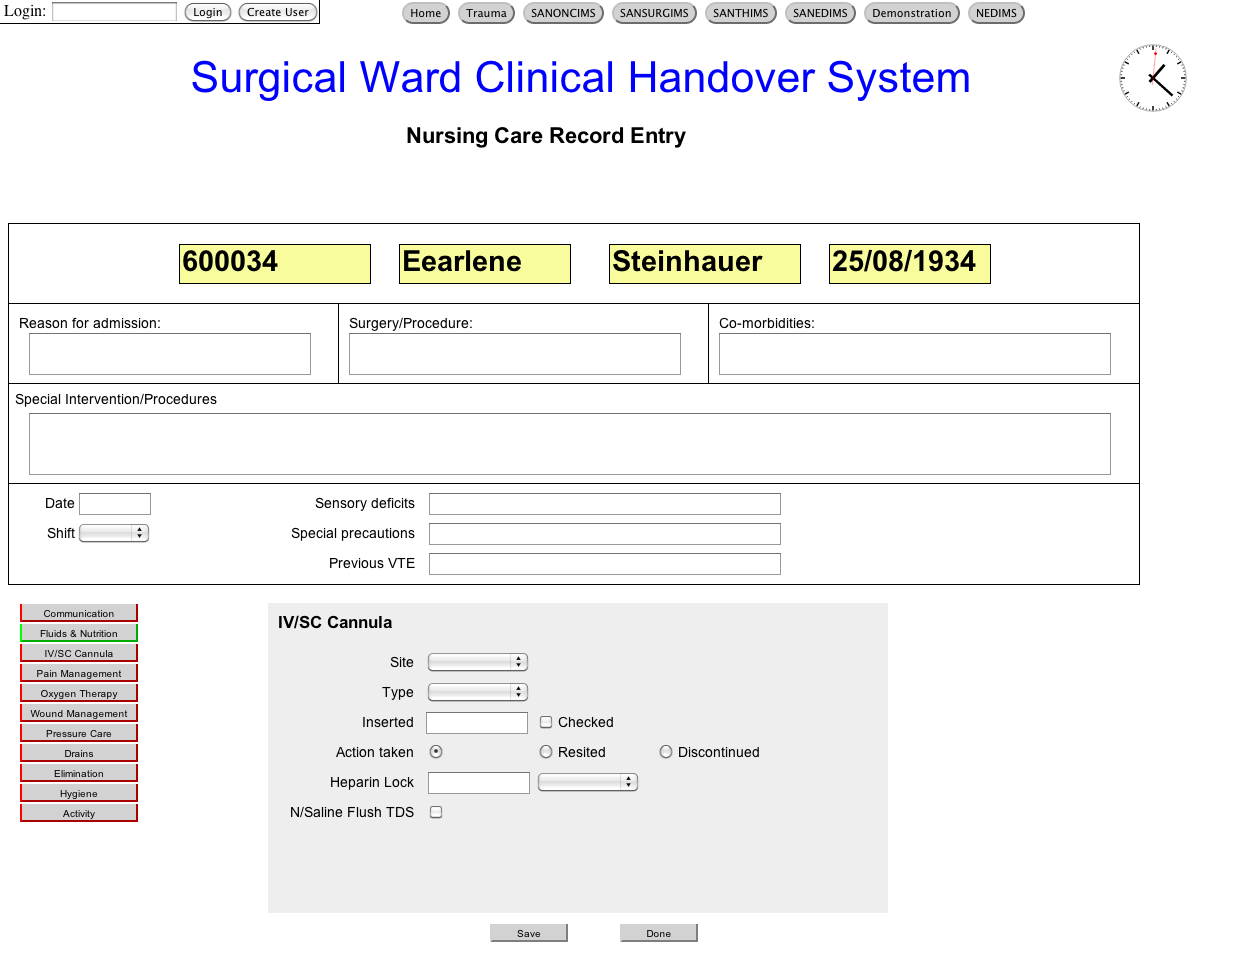
\includegraphics[scale=1.0, width=180mm]{Images/iCIMS-NCRIVSCCannula}
				\caption{Nursing Care Record Entry Form - IV/SC Cannula}
\end{figure} 

\newpage
\begin{figure}[hp]
				\centering
				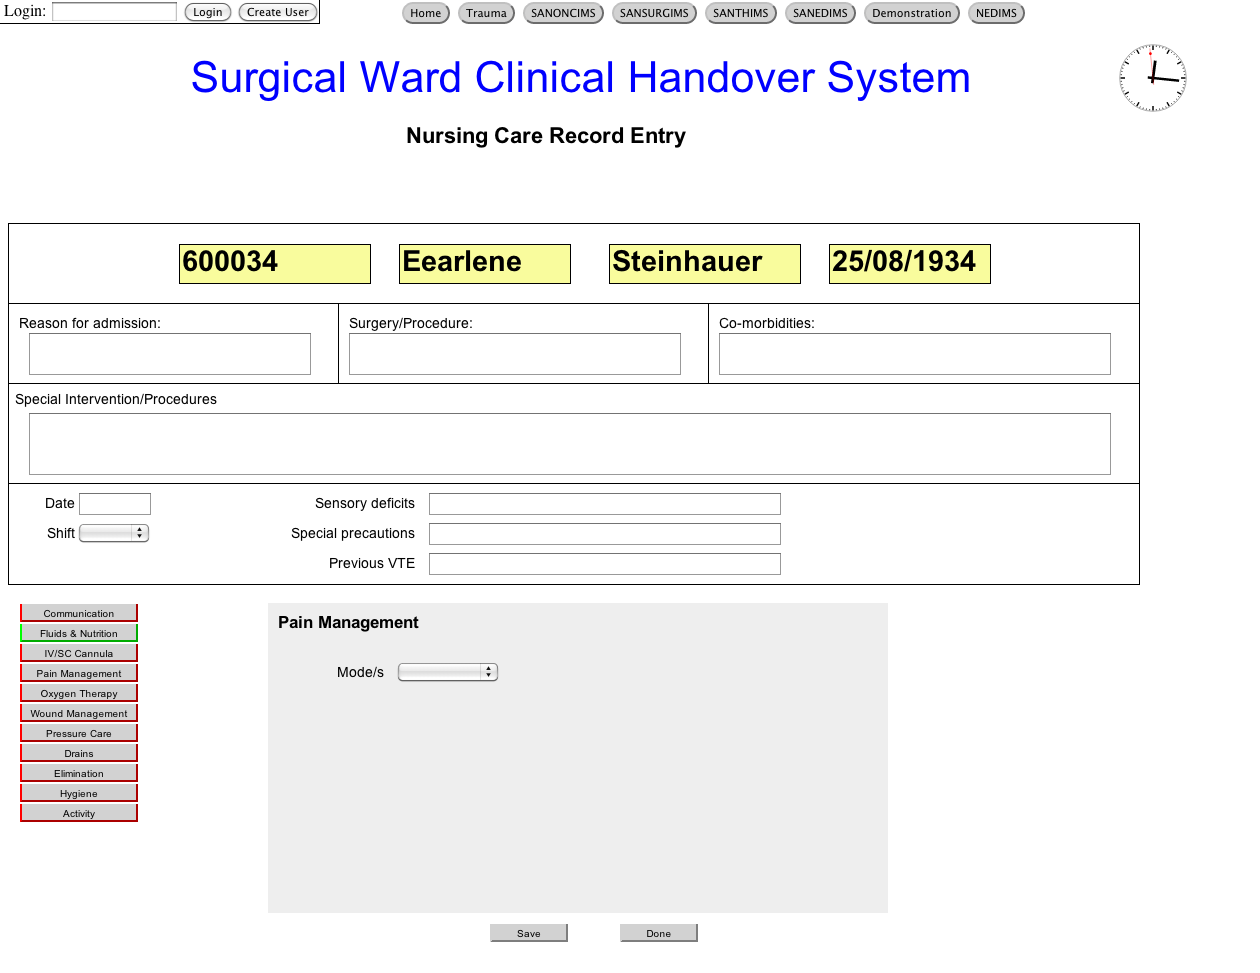
\includegraphics[scale=1.0, width=180mm]{Images/iCIMS-NCRPainManagement}
				\caption{Nursing Care Record Entry Form - Pain Management}
\end{figure} 

\newpage
\begin{figure}[hp]
				\centering
				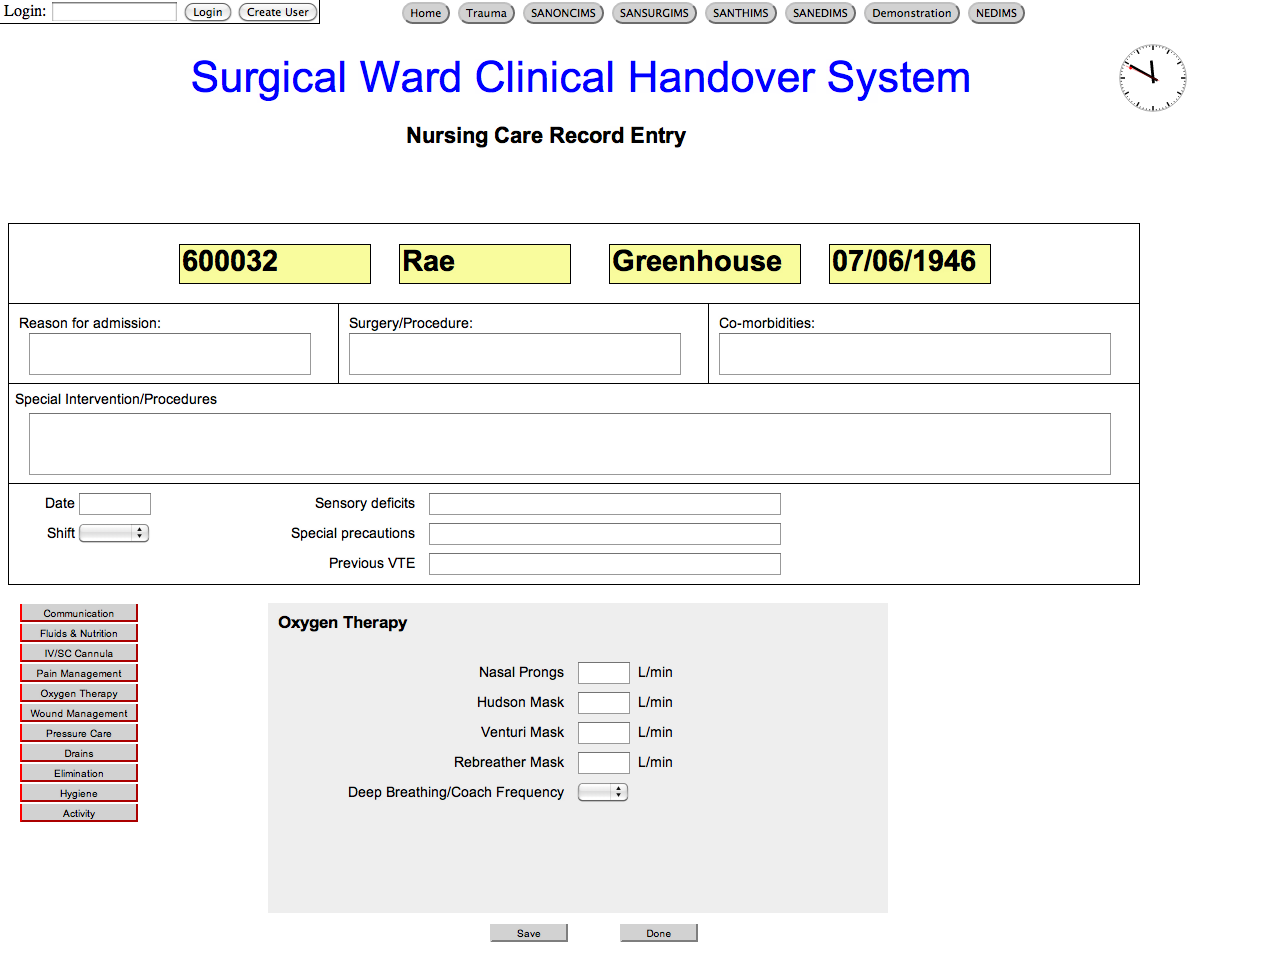
\includegraphics[scale=1.0, width=180mm]{Images/iCIMS-NCROxygenTherapy}
				\caption{Nursing Care Record Entry Form - Oxygen Therapy}
\end{figure} 

\newpage
\begin{figure}[hp]
				\centering
				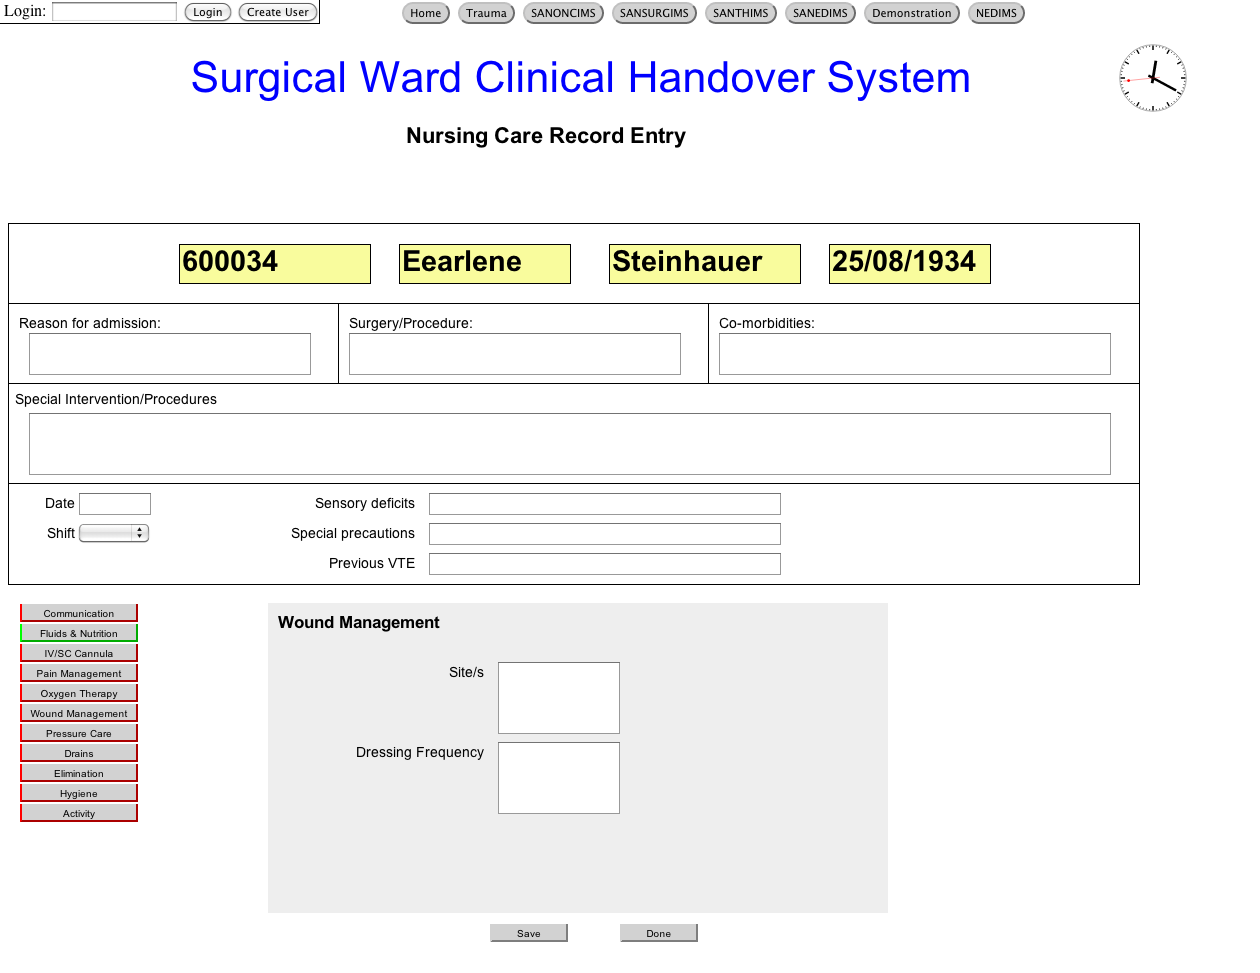
\includegraphics[scale=1.0, width=180mm]{Images/iCIMS-NCRWoundManagement}
				\caption{Nursing Care Record Entry Form - Wound Management}
\end{figure} 

\newpage
\begin{figure}[hp]
				\centering
				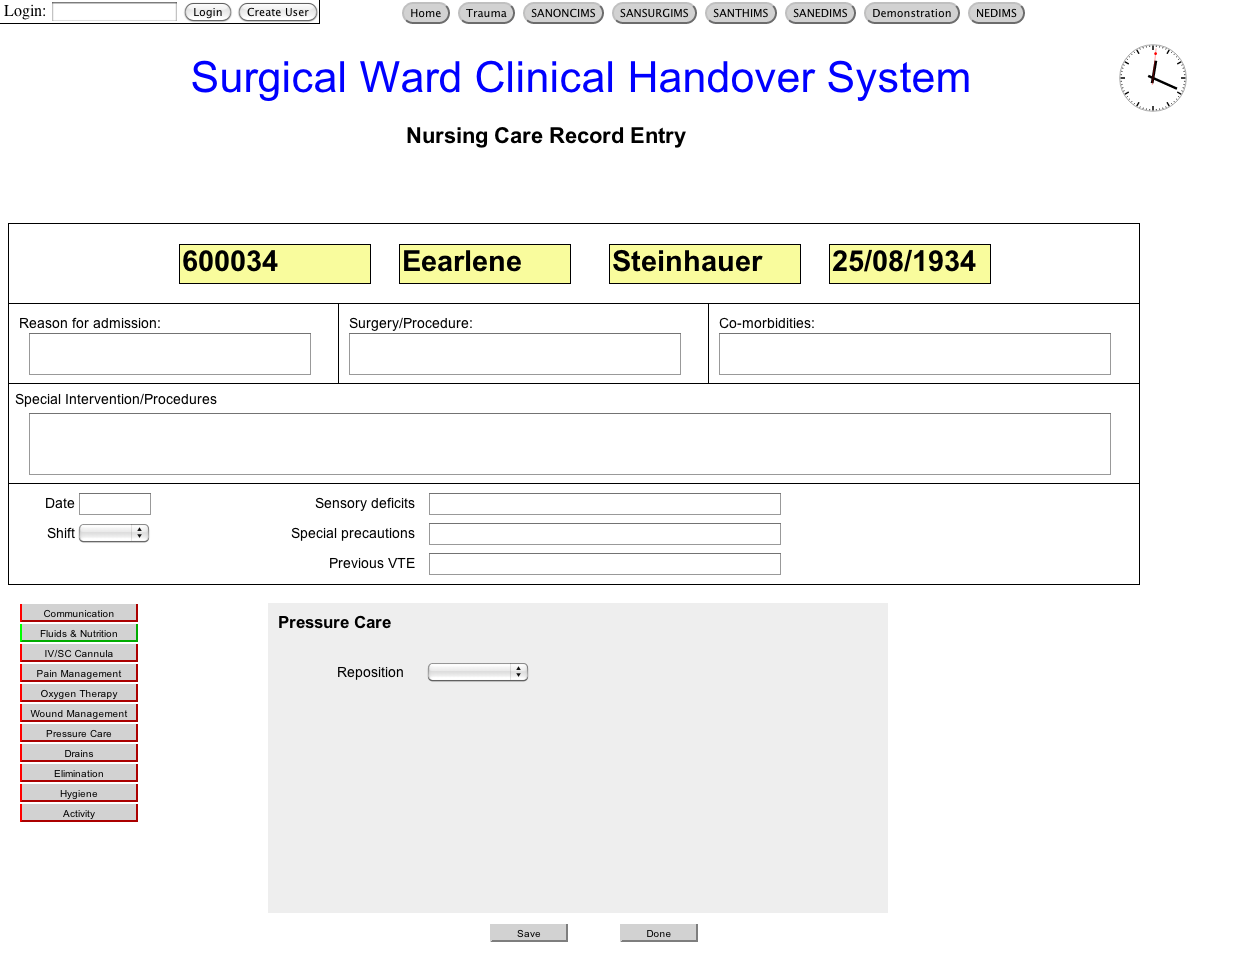
\includegraphics[scale=1.0, width=180mm]{Images/iCIMS-NCRPressureCare}
				\caption{Nursing Care Record Entry Form - Pressure Care}
\end{figure} 

\newpage
\begin{figure}[hp]
				\centering
				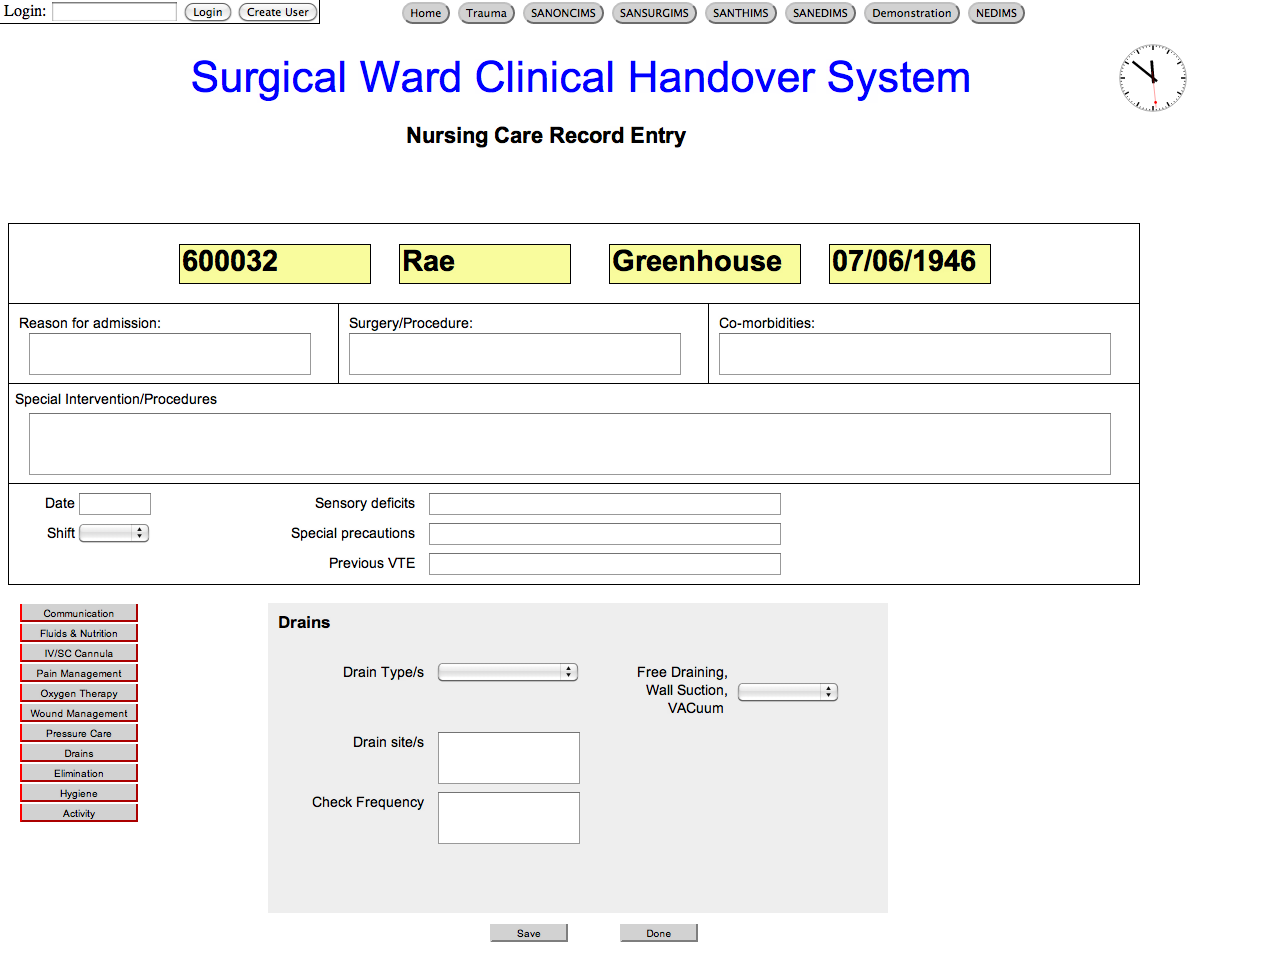
\includegraphics[scale=1.0, width=180mm]{Images/iCIMS-NCRDrains}
				\caption{Nursing Care Record Entry Form - Drains}
\end{figure} 

\newpage
\begin{figure}[hp]
				\centering
				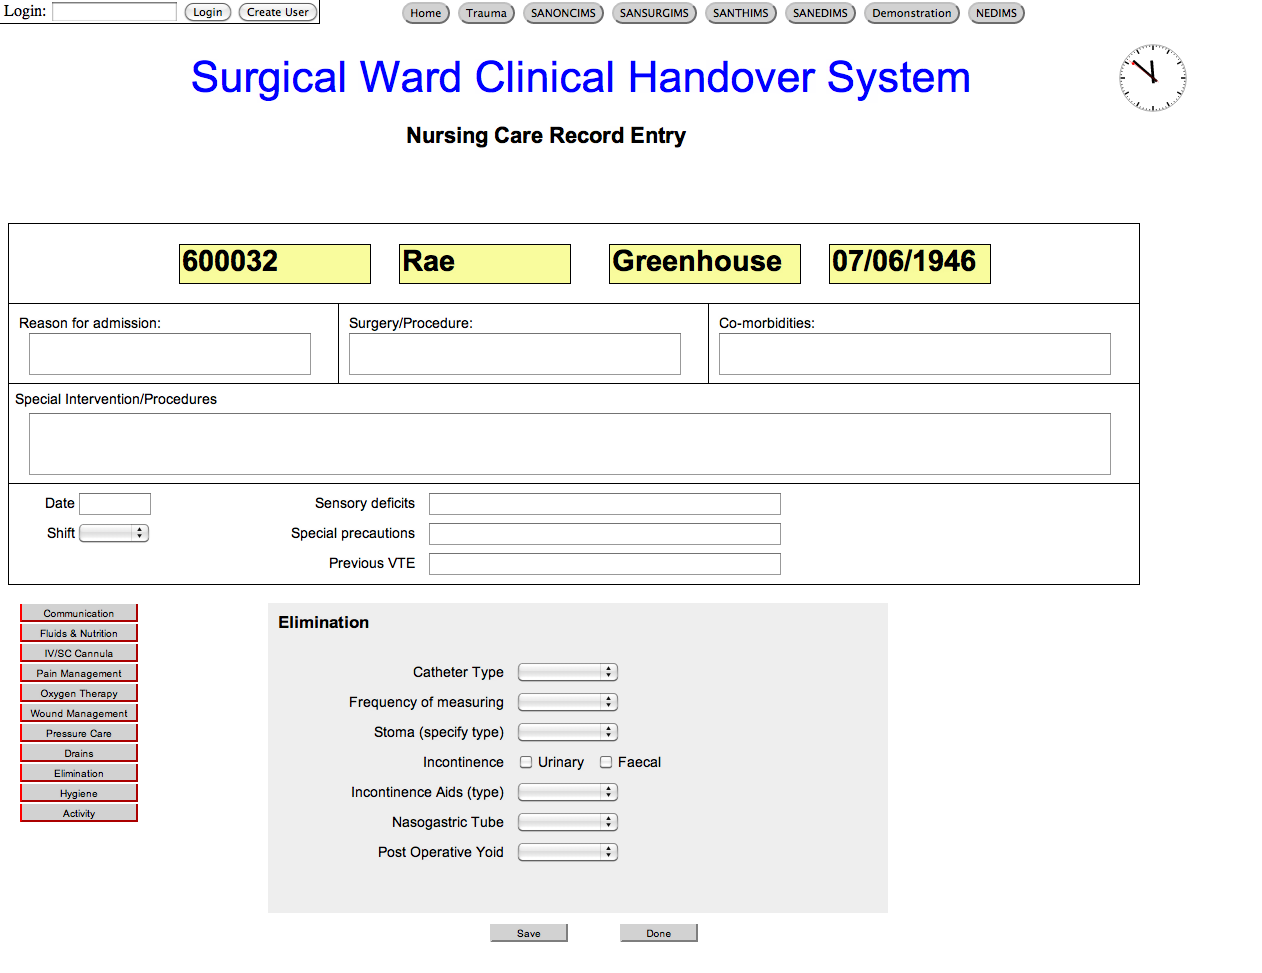
\includegraphics[scale=1.0, width=180mm]{Images/iCIMS-NCRElimination}
				\caption{Nursing Care Record Entry Form - Elimination}
\end{figure} 

\newpage
\begin{figure}[hp]
				\centering
				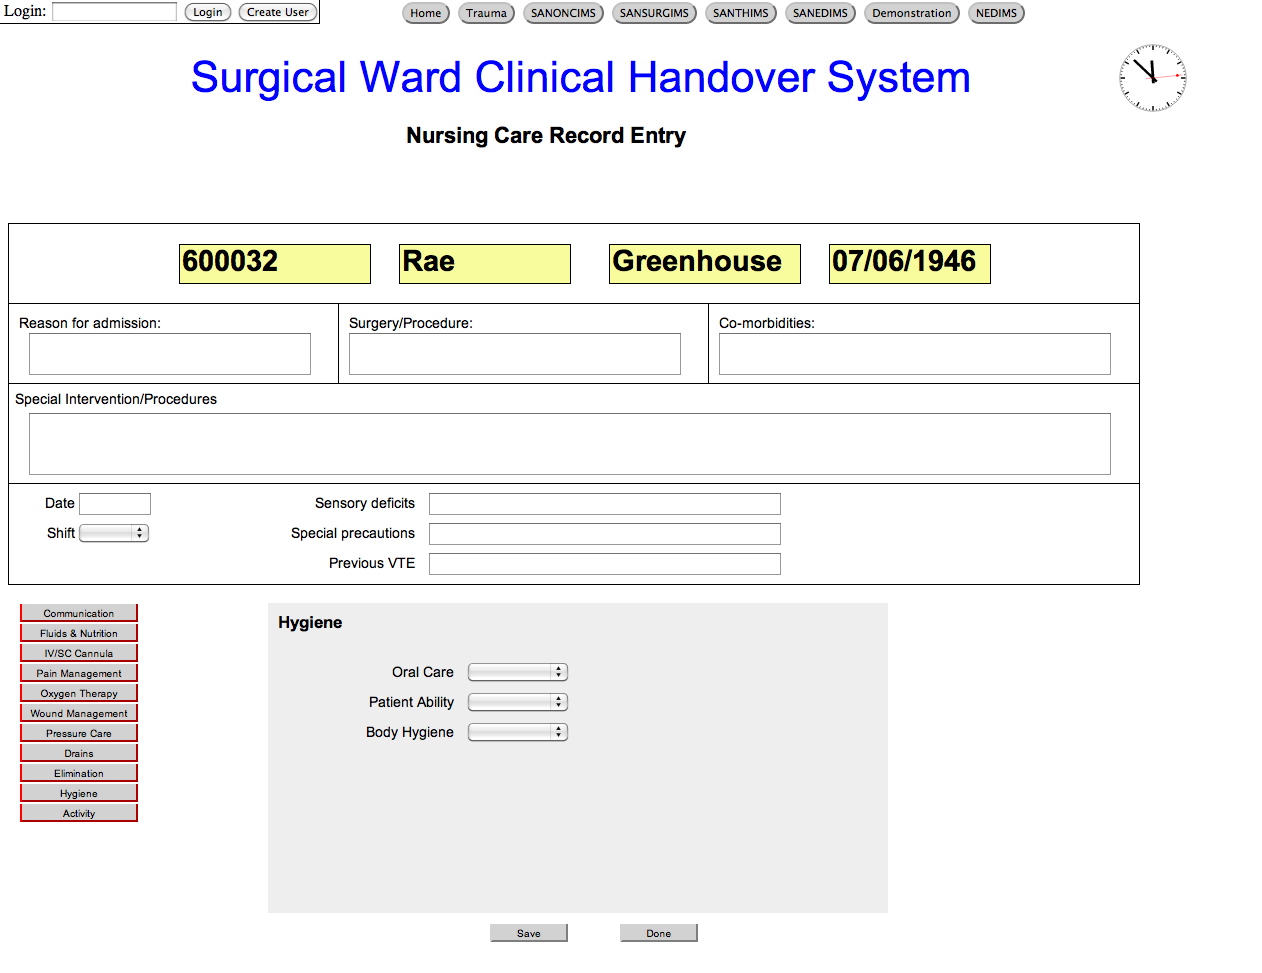
\includegraphics[scale=1.0, width=180mm]{Images/iCIMS-NCRHygiene}
				\caption{Nursing Care Record Entry Form - Hygiene}
\end{figure} 

\newpage
\begin{figure}[hp]
				\centering
				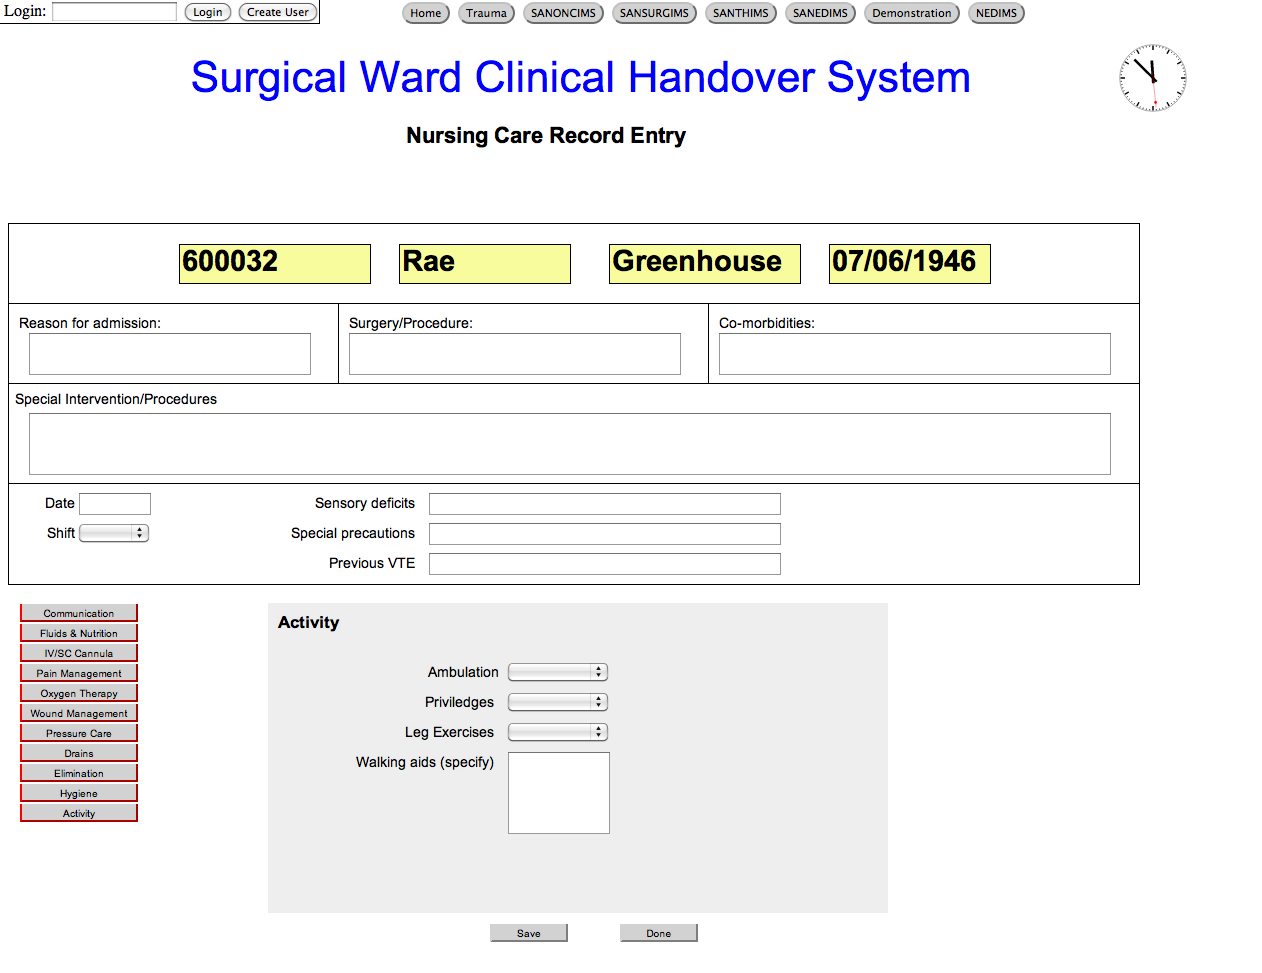
\includegraphics[scale=1.0, width=180mm]{Images/iCIMS-NCRActivity}
				\caption{Nursing Care Record Entry Form - Activity}
\end{figure} 

\newpage
\subsubsection{Nursing Care Record Table Form}
\label{Nursing Care Record Table Form}

\begin{figure}[hp]
				\centering
				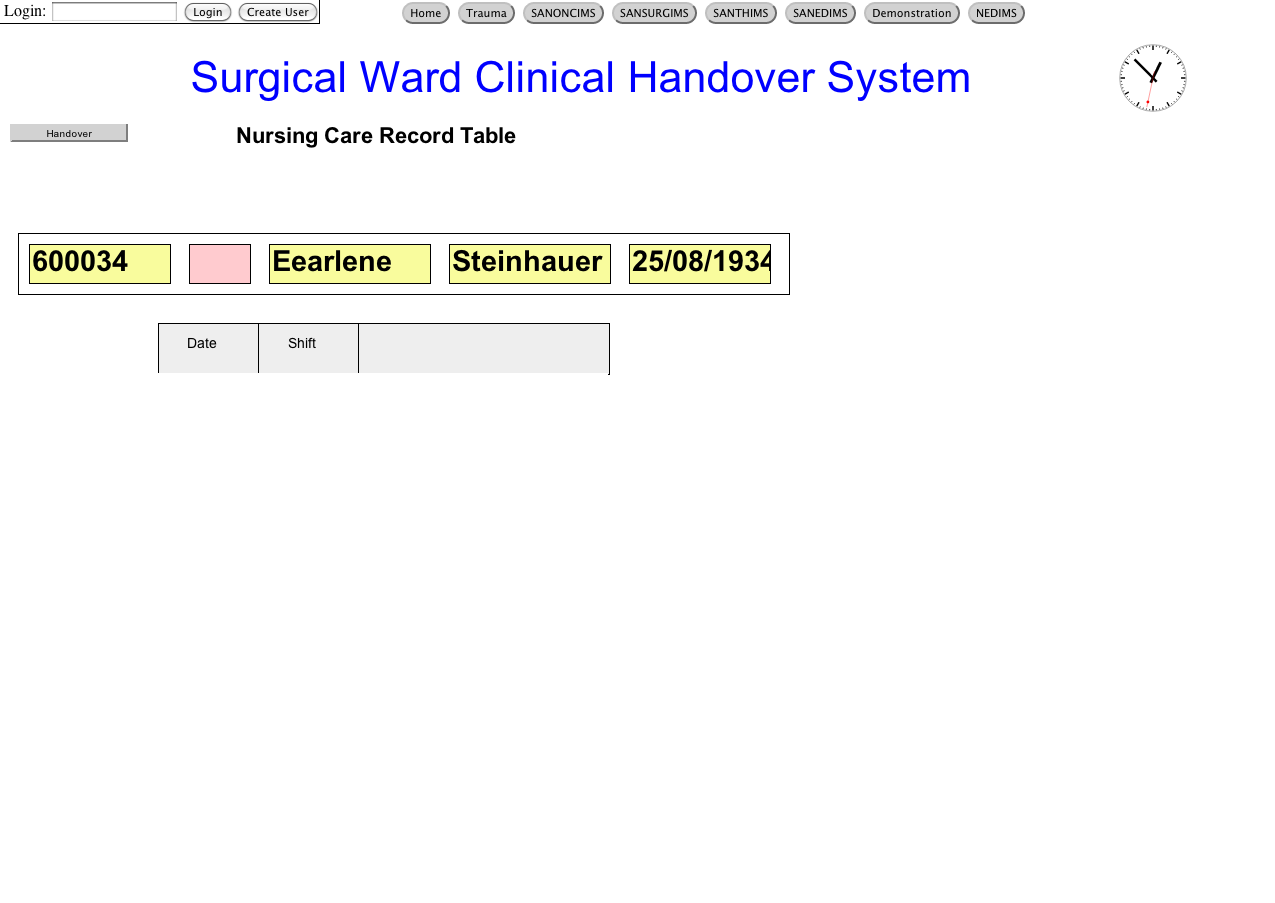
\includegraphics[scale=1.0, width=180mm]{Images/iCIMS-NCRTable}
				\caption{Nursing Care Record Table Form}
\end{figure}

\newpage
\subsubsection{Patient History Form}
\label{Patient History Form}
Created by Jenny Kongkalai in SANONCIMS.

\begin{figure}[hp]
				\centering
				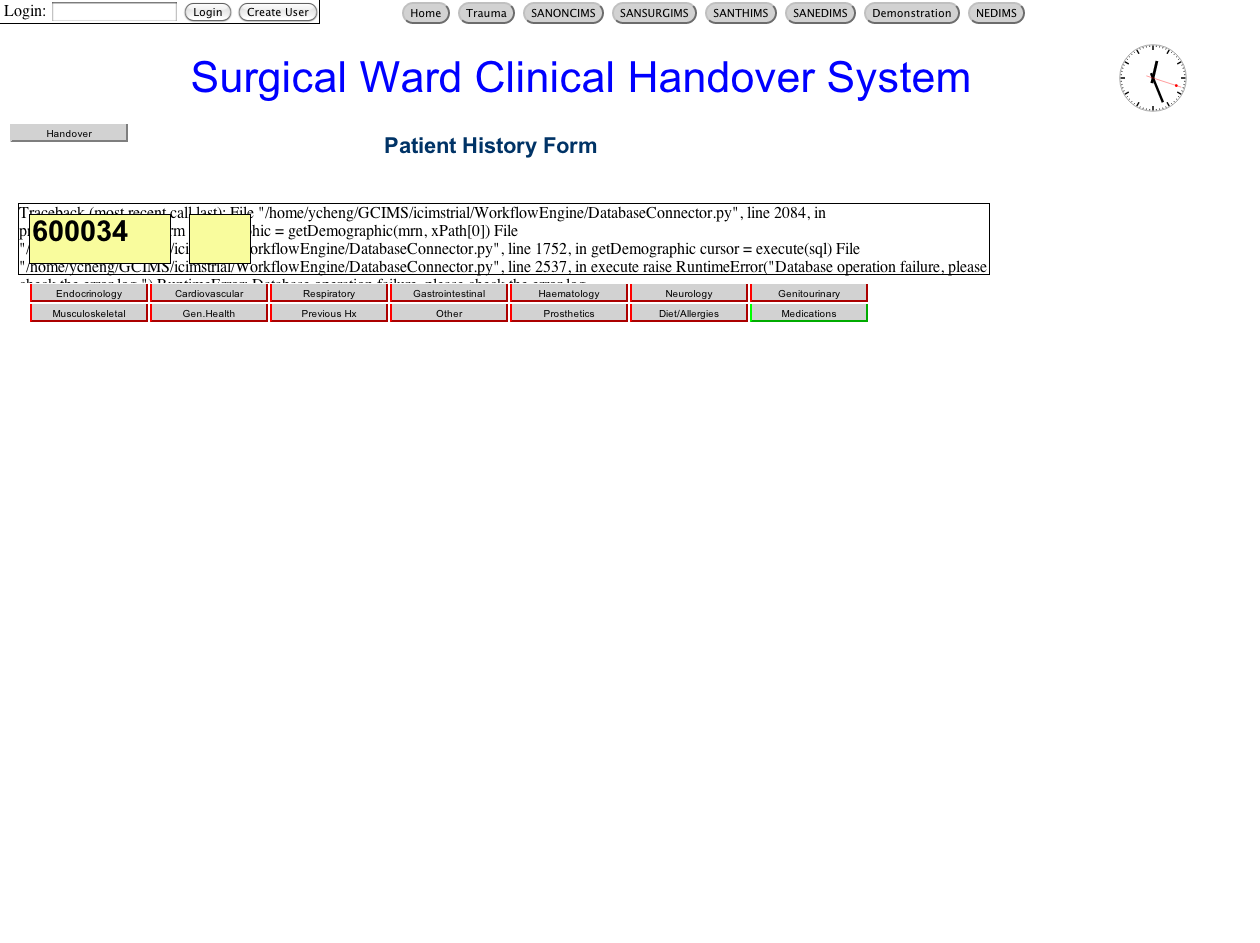
\includegraphics[scale=1.0, width=180mm]{Images/iCIMS-PatientHistory-Jenny}
				\caption{Patient History Form}
\end{figure}

\newpage
\subsubsection{Patient Mobility Assessment Form}
\label{Patient Mobility Assessment Form}

\begin{figure}[hp]
				\centering
				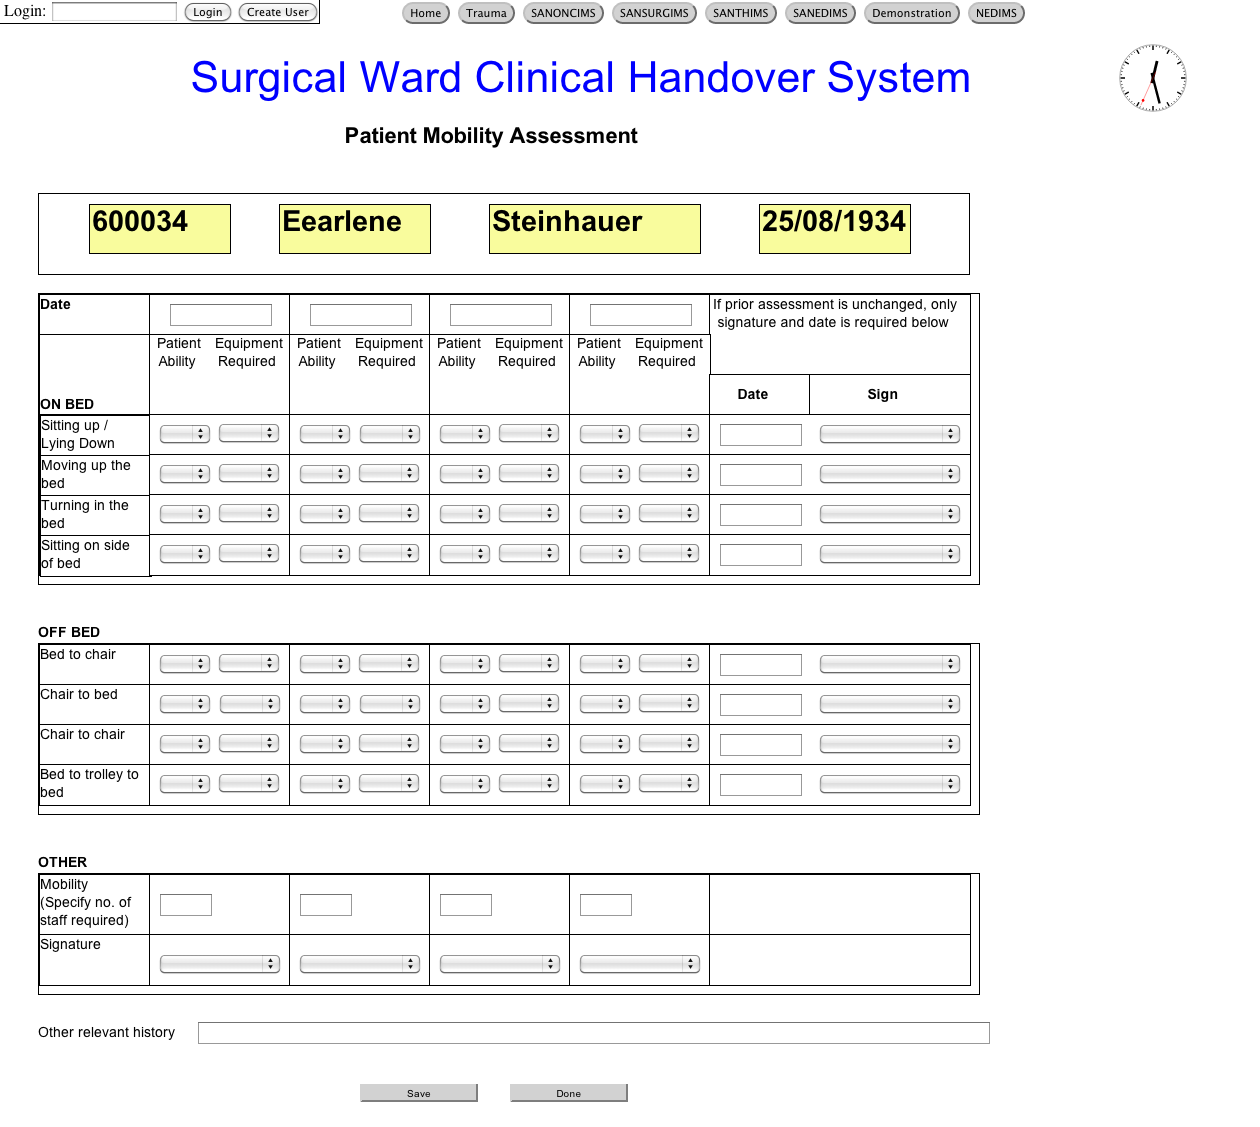
\includegraphics[scale=1.0, width=180mm]{Images/iCIMS-PatientMobilityAssessment}
				\caption{Patient Mobility Assessment Form}
\end{figure}

\newpage
\subsubsection{Observation Chart Entry Form}
\label{Observation Chart Entry Form}

\begin{figure}[hp]
				\centering
				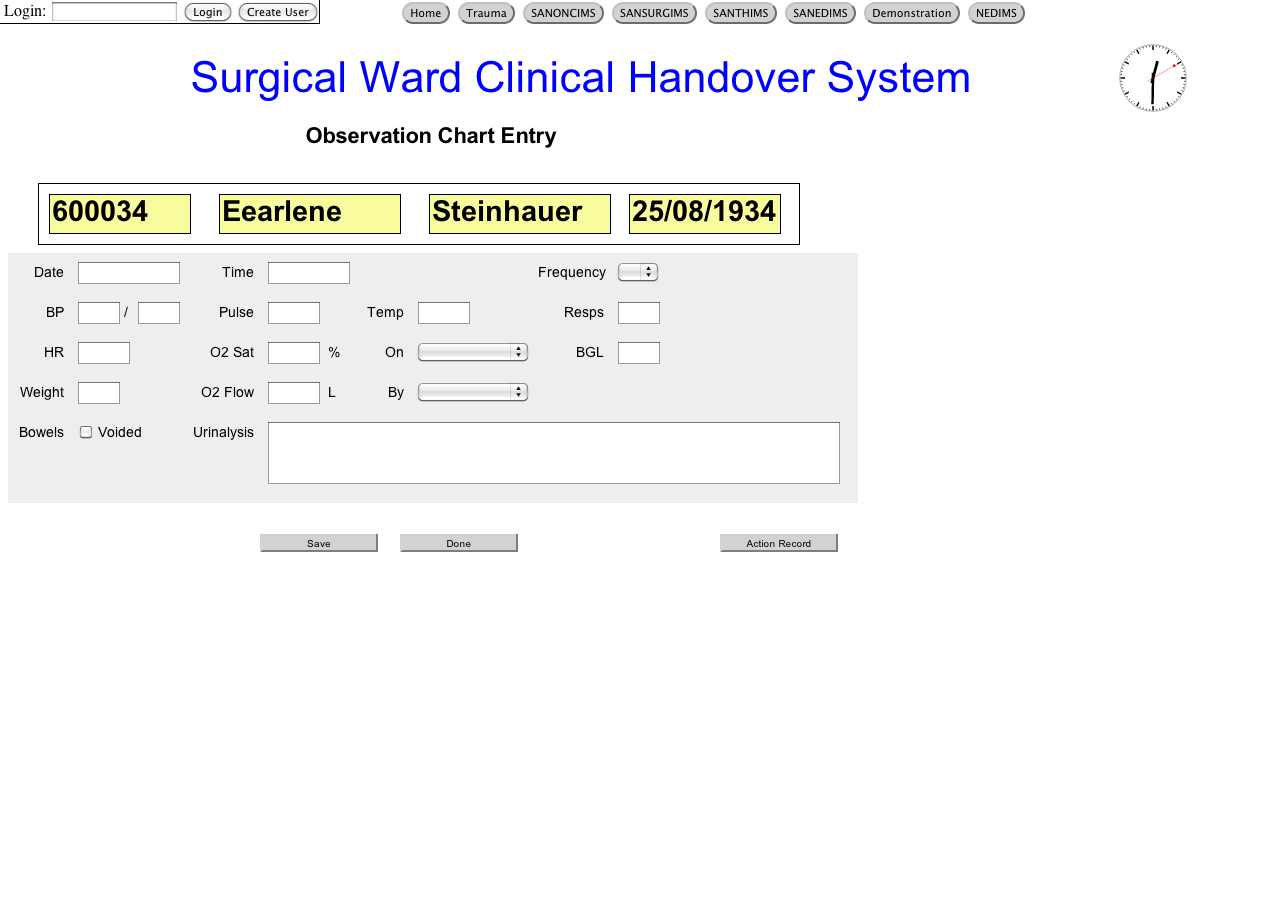
\includegraphics[scale=1.0, width=180mm]{Images/iCIMS-AdultObsEntry}
				\caption{Observation Chart Entry Form}
\end{figure}

\newpage
\subsubsection{Observation Chart Table Form}
\label{Observation Chart Table Form}

\begin{figure}[hp]
				\centering
				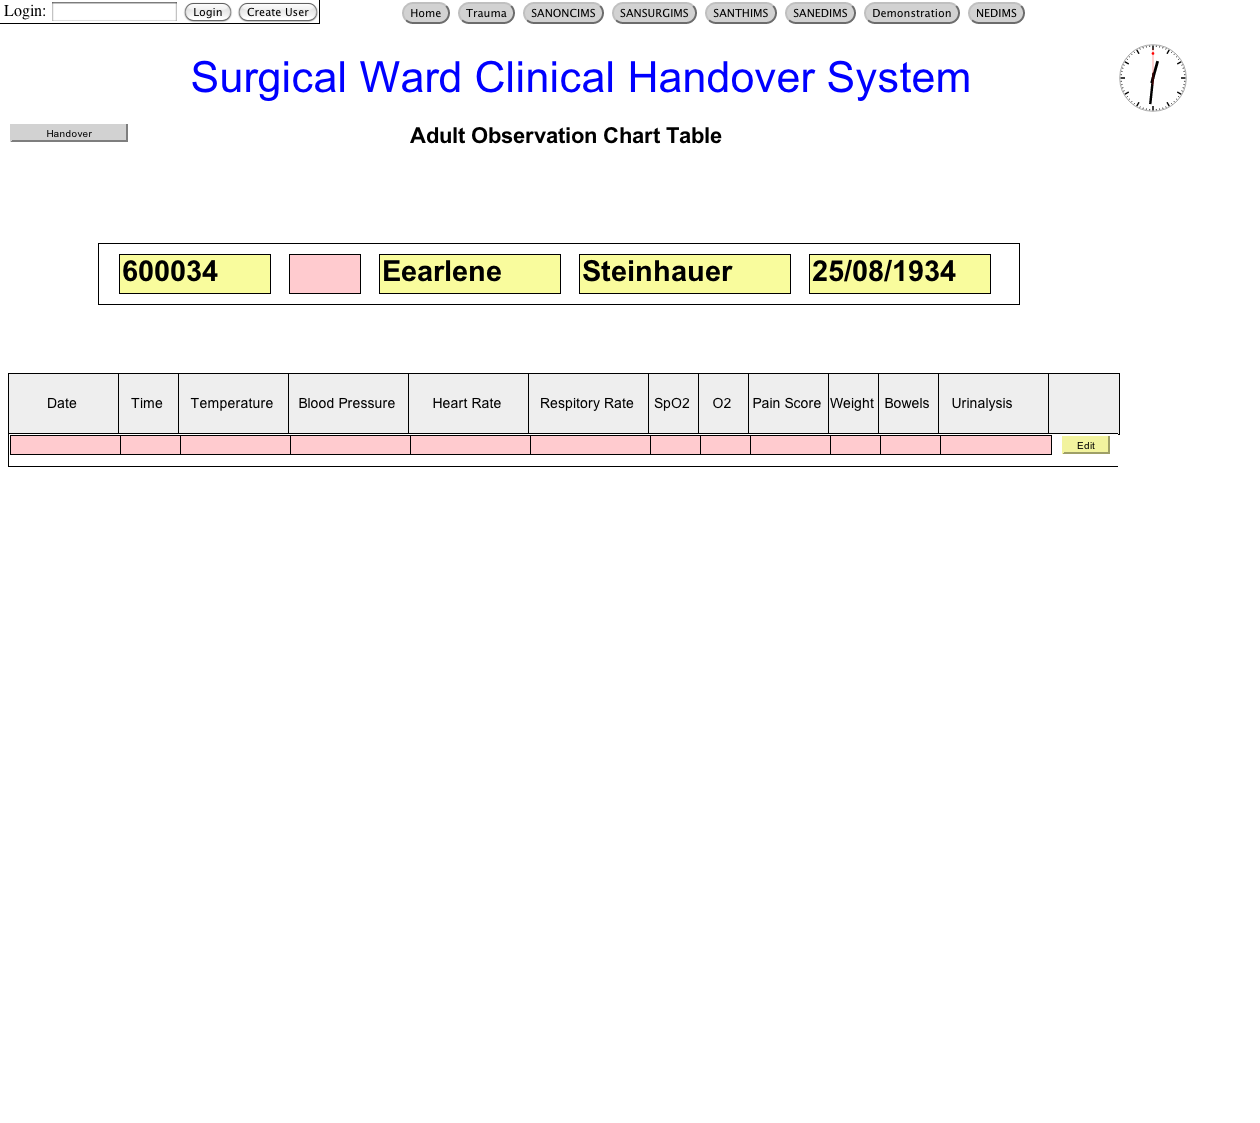
\includegraphics[scale=1.0, width=180mm]{Images/iCIMS-AdultObsTable}
				\caption{Observation Chart Table Form}
\end{figure}

\newpage
\subsubsection{Action Record Entry Form}
\label{Action Record Entry Form}

\begin{figure}[hp]
				\centering
				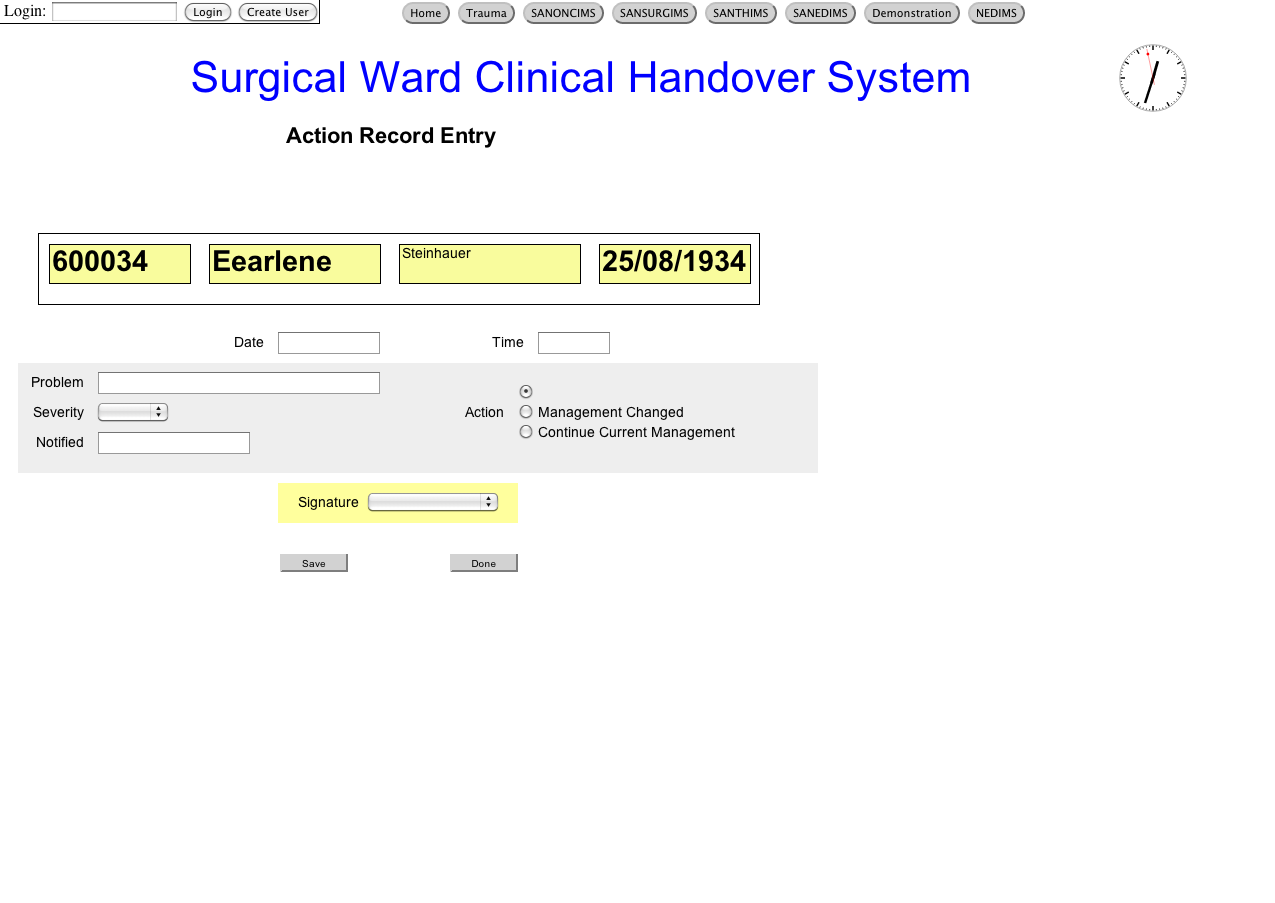
\includegraphics[scale=1.0, width=180mm]{Images/iCIMS-ActionRecordEntry}
				\caption{Action Record Entry Form}
\end{figure}

\newpage
\subsubsection{Action Record Table Form}
\label{Action Record Table Form}

\begin{figure}[hp]
				\centering
				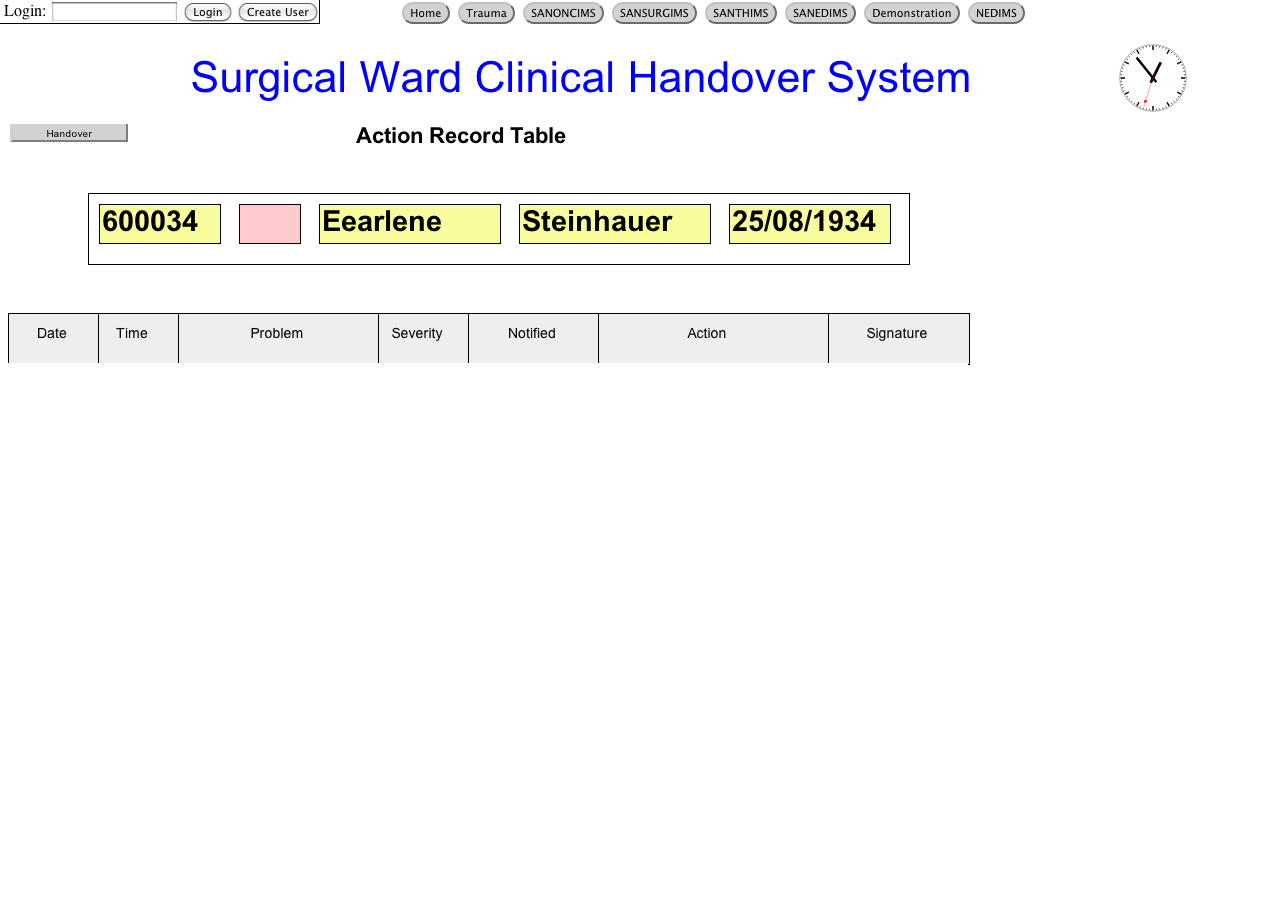
\includegraphics[scale=1.0, width=180mm]{Images/iCIMS-ActionRecordTable}
				\caption{Action Record Table Form}
\end{figure}

\newpage
\subsubsection{Nurse Risk Screening and Assessment Form}
\label{Nurse Risk Screening and Assessment Form}
Created by Jenny Kongkalai in SANONCIMS.

\begin{figure}[hp]
				\centering
				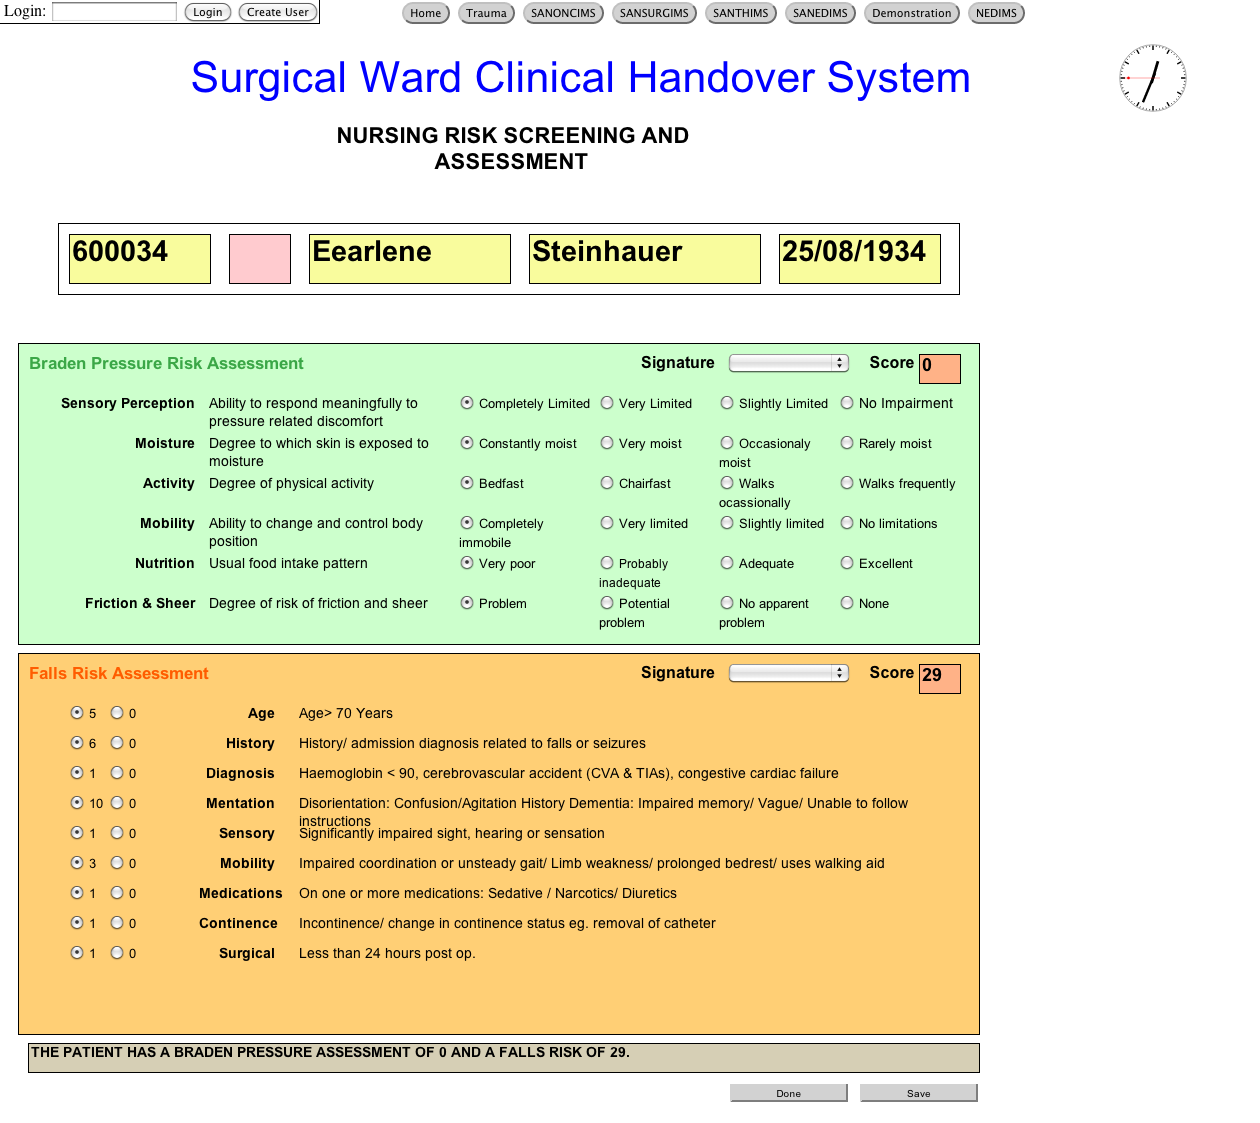
\includegraphics[scale=1.0, width=180mm]{Images/iCIMS-NurseRiskScreening}
				\caption{Nurse Risk Screening and Assessment Form}
\end{figure}

\newpage
\subsubsection{Admin Screen Form}
\label{Admin Screen Form}

\begin{figure}[hp]
				\centering
				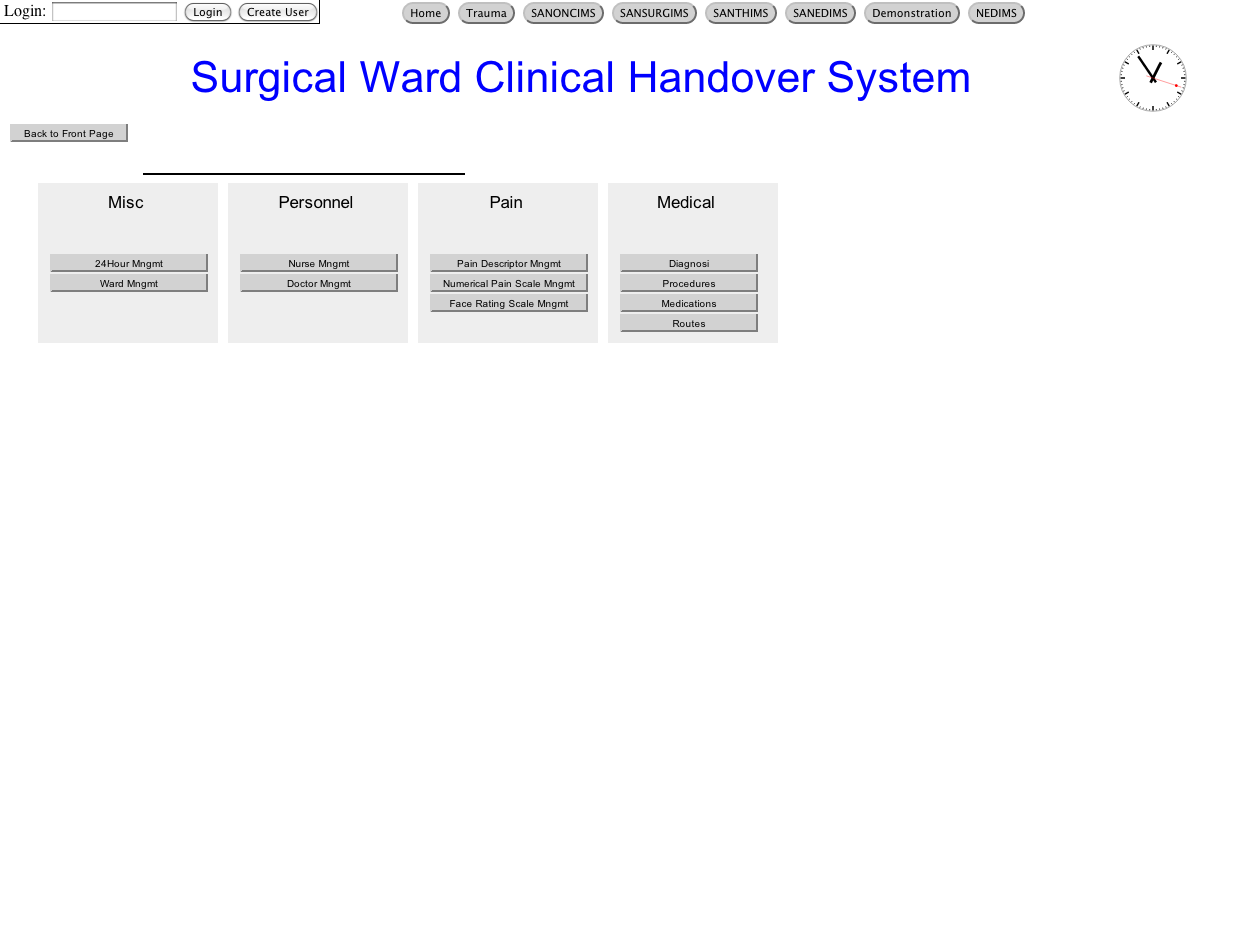
\includegraphics[scale=1.0, width=180mm]{Images/iCIMS-AdminScreen}
				\caption{Admin Screen Form}
\end{figure}

\newpage
\subsubsection{Allergy Form}
\label{Allergy Form}

\begin{figure}[hp]
				\centering
				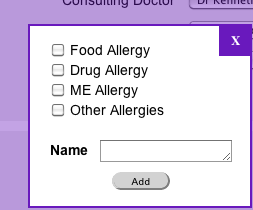
\includegraphics[scale=1.0, width=60mm]{Images/iCIMS-Allergy}
				\caption{Allergy Form}
\end{figure}

\subsubsection{Comorbidity Form}
\label{Comorbidity Form}

\begin{figure}[hp]
				\centering
				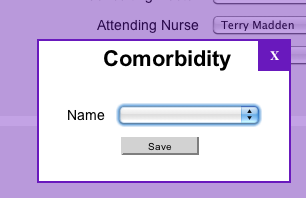
\includegraphics[scale=1.0, width=60mm]{Images/iCIMS-Comorbidity}
				\caption{Comorbidity Form}
\end{figure}

\subsubsection{Visual Impairments Form}
\label{Visual Impairments Form}

\begin{figure}[hp]
				\centering
				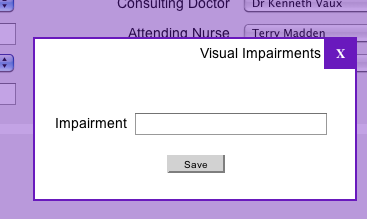
\includegraphics[scale=1.0, width=60mm]{Images/iCIMS-VisualImpairment}
				\caption{Visual Impairments Form}
\end{figure}

\newpage
\subsubsection{Fluid Balance Chart Entry Form}
\label{Fluid Balance Chart Entry Form}

\begin{figure}[hp]
				\centering
				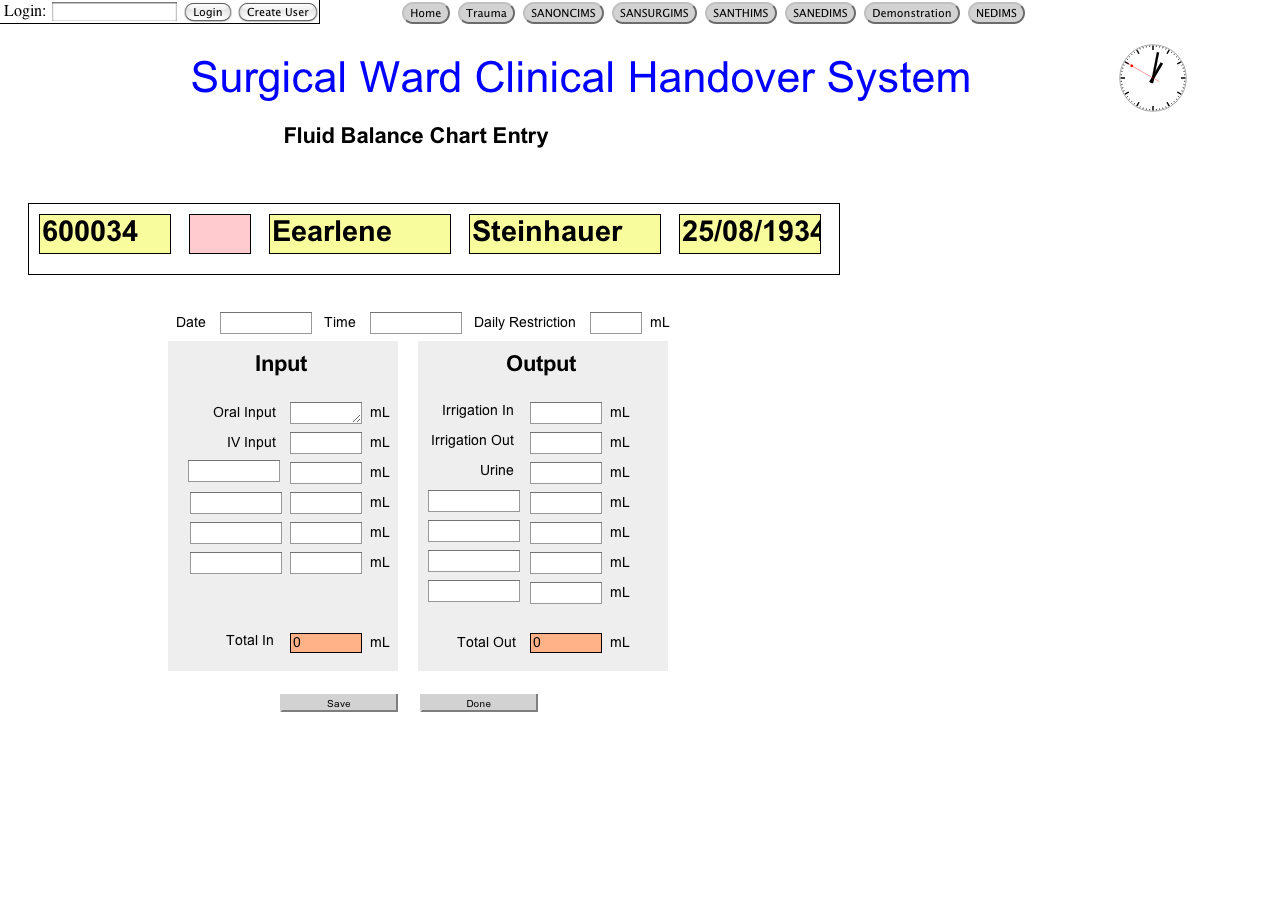
\includegraphics[scale=1.0, width=180mm]{Images/iCIMS-FluidBalanceEntry}
				\caption{Fluid Balance Chart Entry Form}
\end{figure}

\newpage
\subsubsection{Fluid Balance Chart Table Form}
\label{Fluid Balance Chart Table Form}

\begin{figure}[hp]
				\centering
				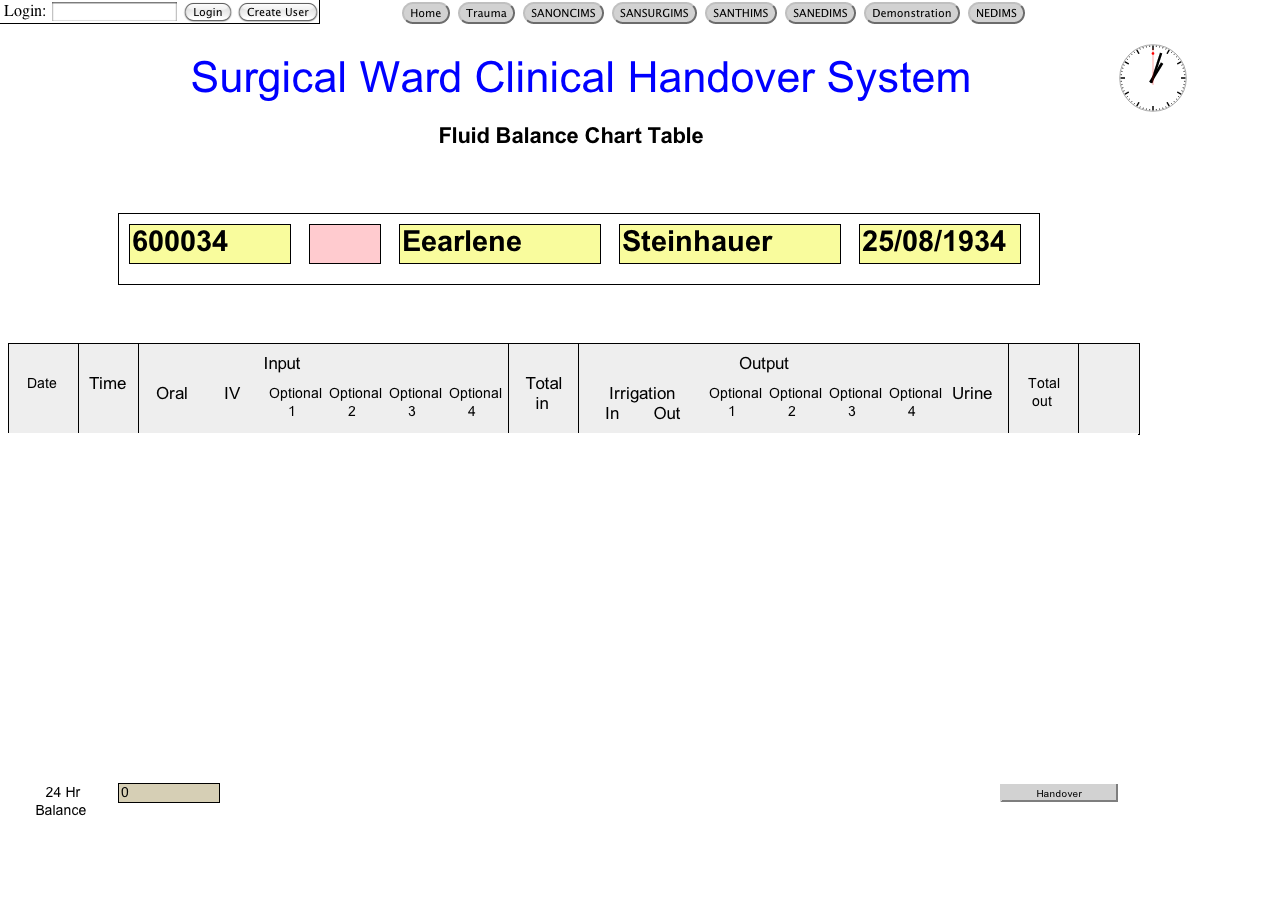
\includegraphics[scale=1.0, width=180mm]{Images/iCIMS-FluidBalanceTable}
				\caption{Fluid Balance Chart Table Form}
\end{figure}

\newpage
\subsubsection{Emergency Order Entry Form}
\label{Emergency Order Entry Form}

\begin{figure}[hp]
				\centering
				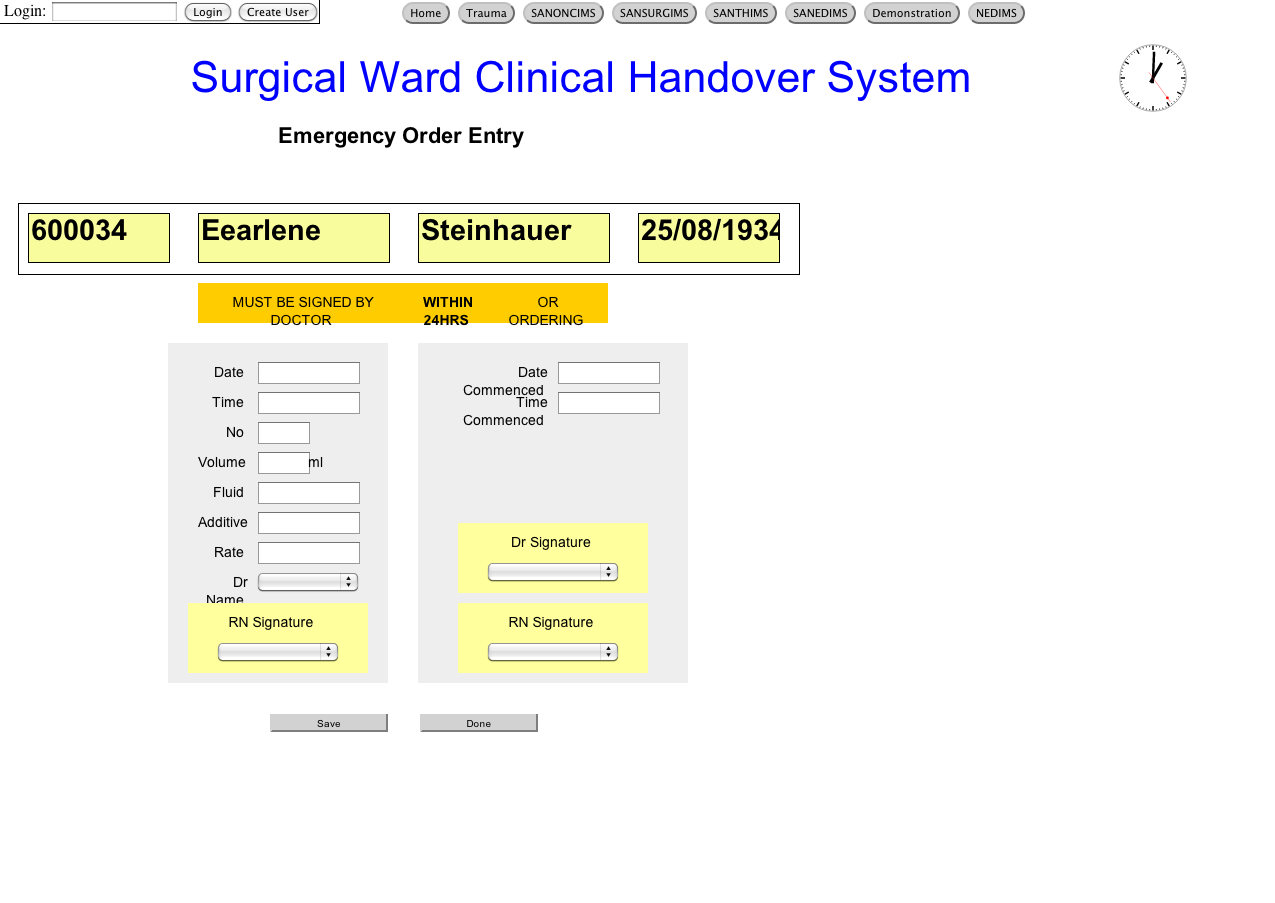
\includegraphics[scale=1.0, width=180mm]{Images/iCIMS-EmergencyOrderEntry}
				\caption{Emergency Order Entry Form}
\end{figure}

\newpage
\subsubsection{Intravenous Fluid Order Entry Form}
\label{Intravenous Fluid Order Entry Form}

\begin{figure}[hp]
				\centering
				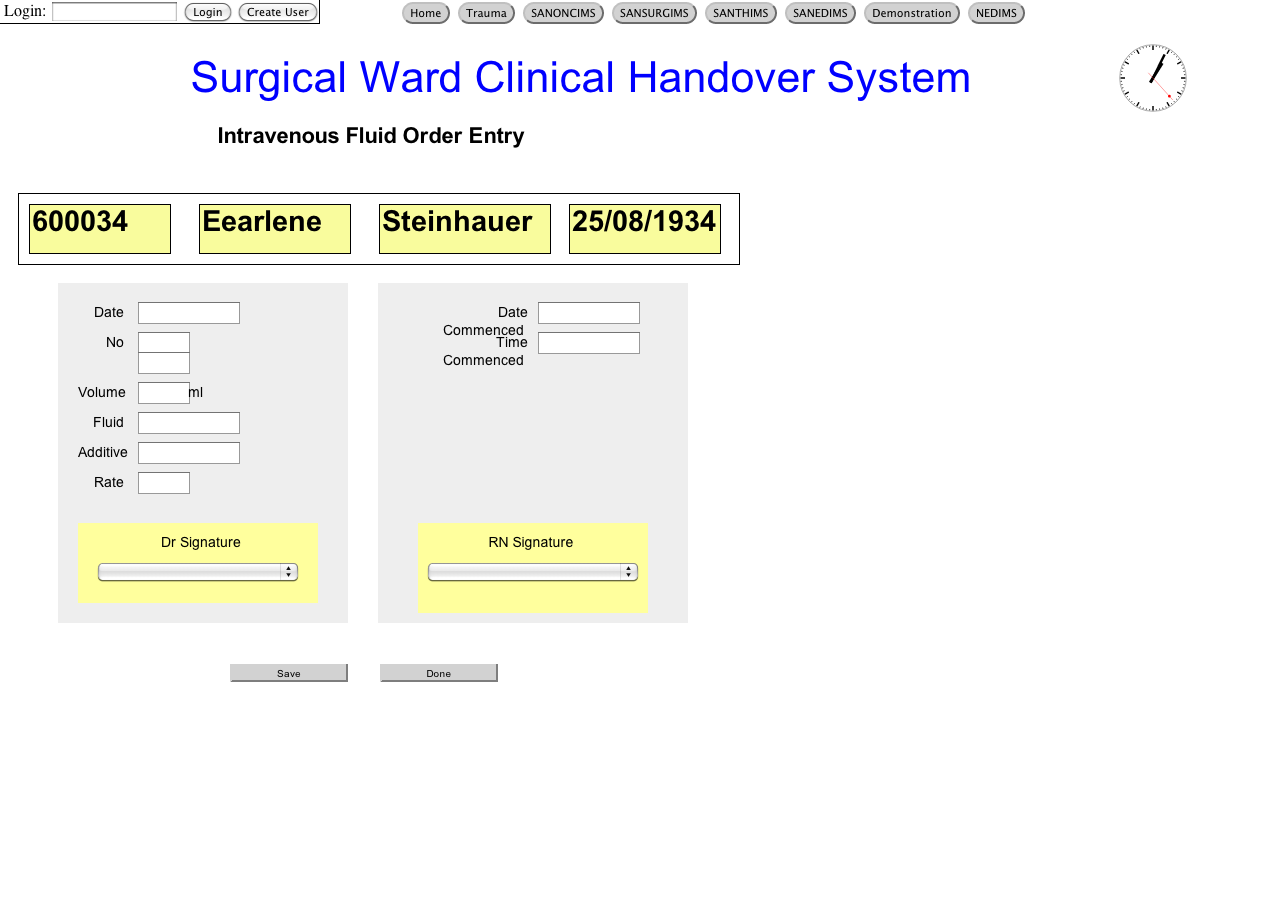
\includegraphics[scale=1.0, width=180mm]{Images/iCIMS-IntravenousFluidEntry}
				\caption{Intravenous Fluid Order Entry Form}
\end{figure}

\newpage
\subsubsection{Intravenous Fluid Orders and Emergency Orders Form}
\label{Intravenous Fluid Orders and Emergency Orders Form}

\begin{figure}[hp]
				\centering
				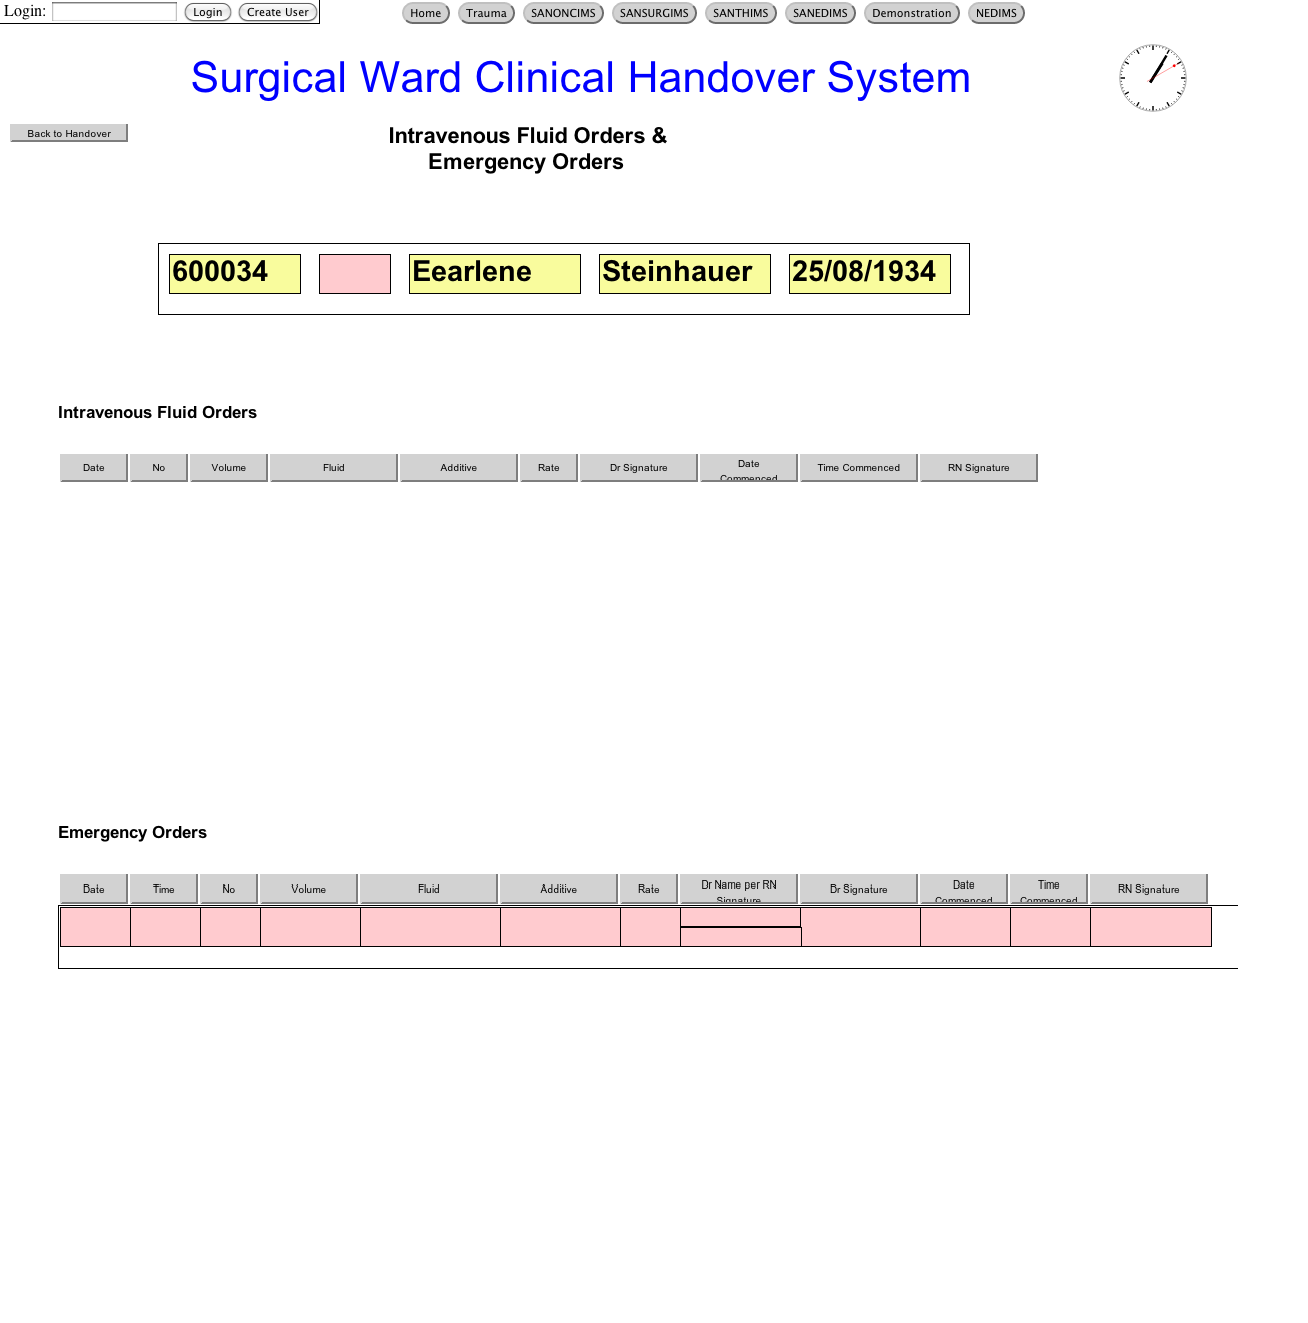
\includegraphics[scale=1.0, width=160mm]{Images/iCIMS-IVFluidEmergencyOrderTable}
				\caption{Intravenous Fluid Orders and Emergency Orders Form}
\end{figure}

\newpage
\subsubsection{Once Only, Pre-Medication and Nurse Initiated Medicines Form}
\label{Once Only, Pre-Medication and Nurse Initiated Medicines Form}

\begin{figure}[hp]
				\centering
				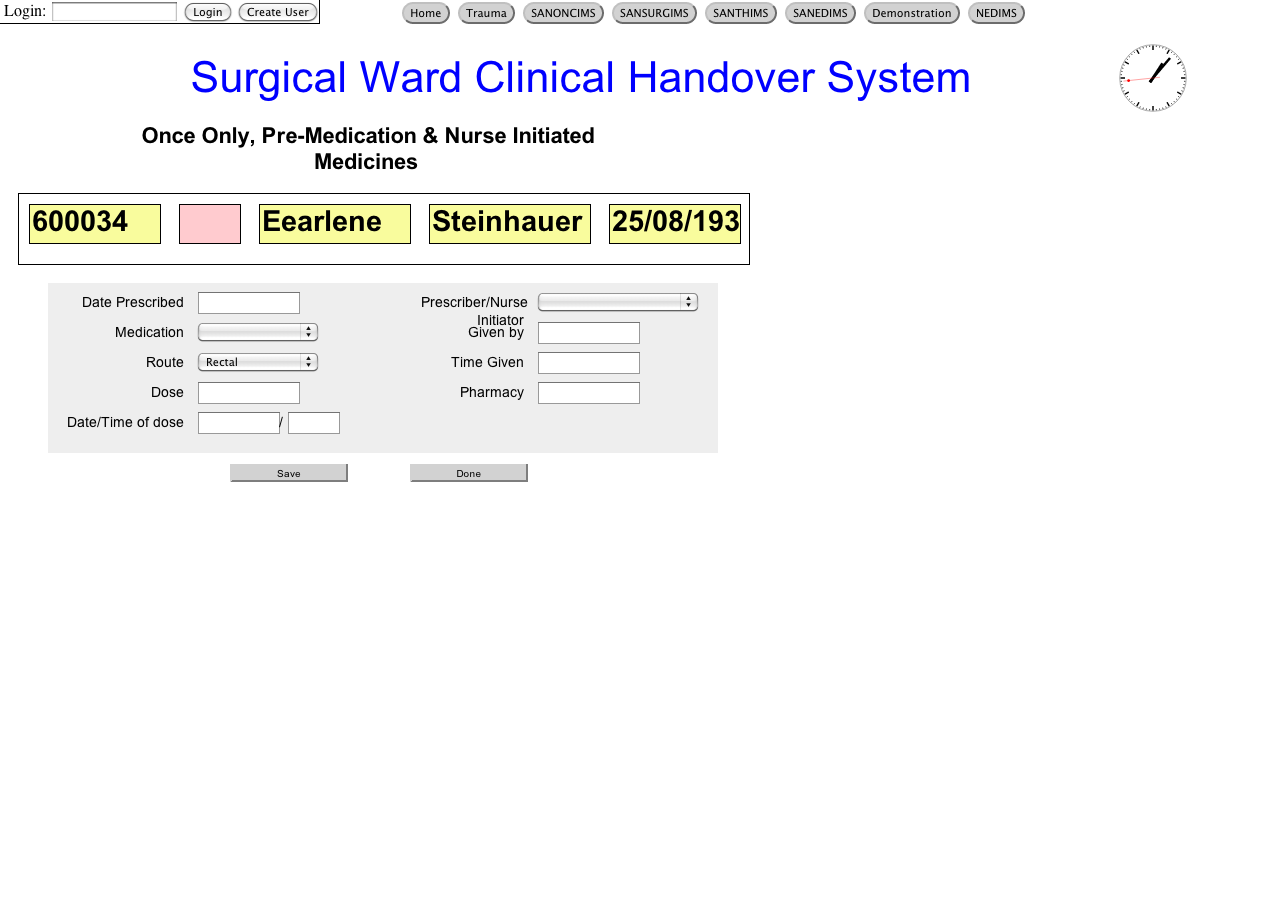
\includegraphics[scale=1.0, width=180mm]{Images/iCIMS-OnceOnlyNurseInitMeds}
				\caption{Once Only, Pre-Medication and Nurse Initiated Medicines Form}
\end{figure}

\newpage
\subsubsection{Telephone Order Entry Form}
\label{Telephone Order Entry Form}

\begin{figure}[hp]
				\centering
				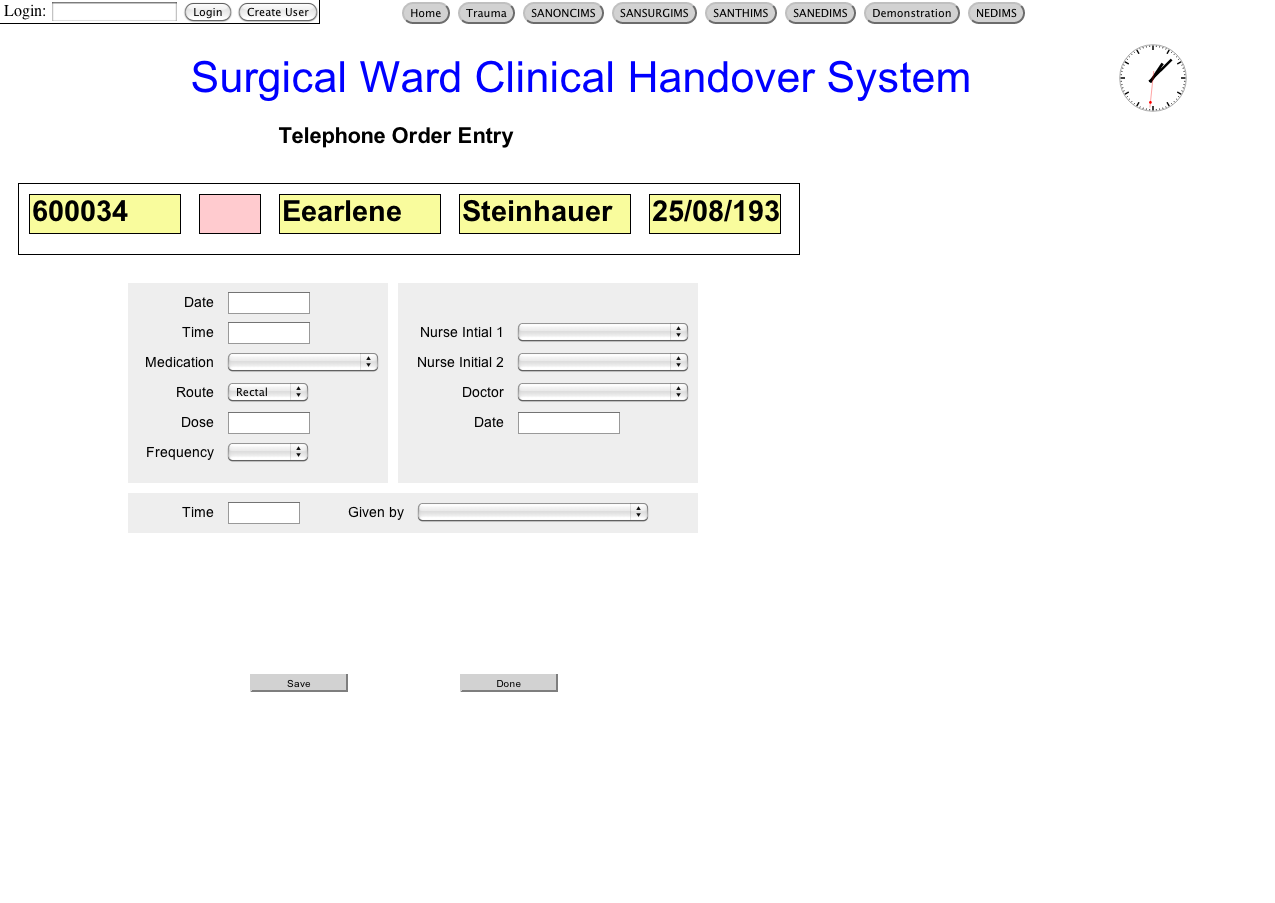
\includegraphics[scale=1.0, width=180mm]{Images/iCIMS-TelephoneOrderEntry}
				\caption{Telephone Order Entry Form}
\end{figure}

\newpage
\subsubsection{Medication Chart Form}
\label{Medication Chart Form}

\begin{figure}[hp]
				\centering
				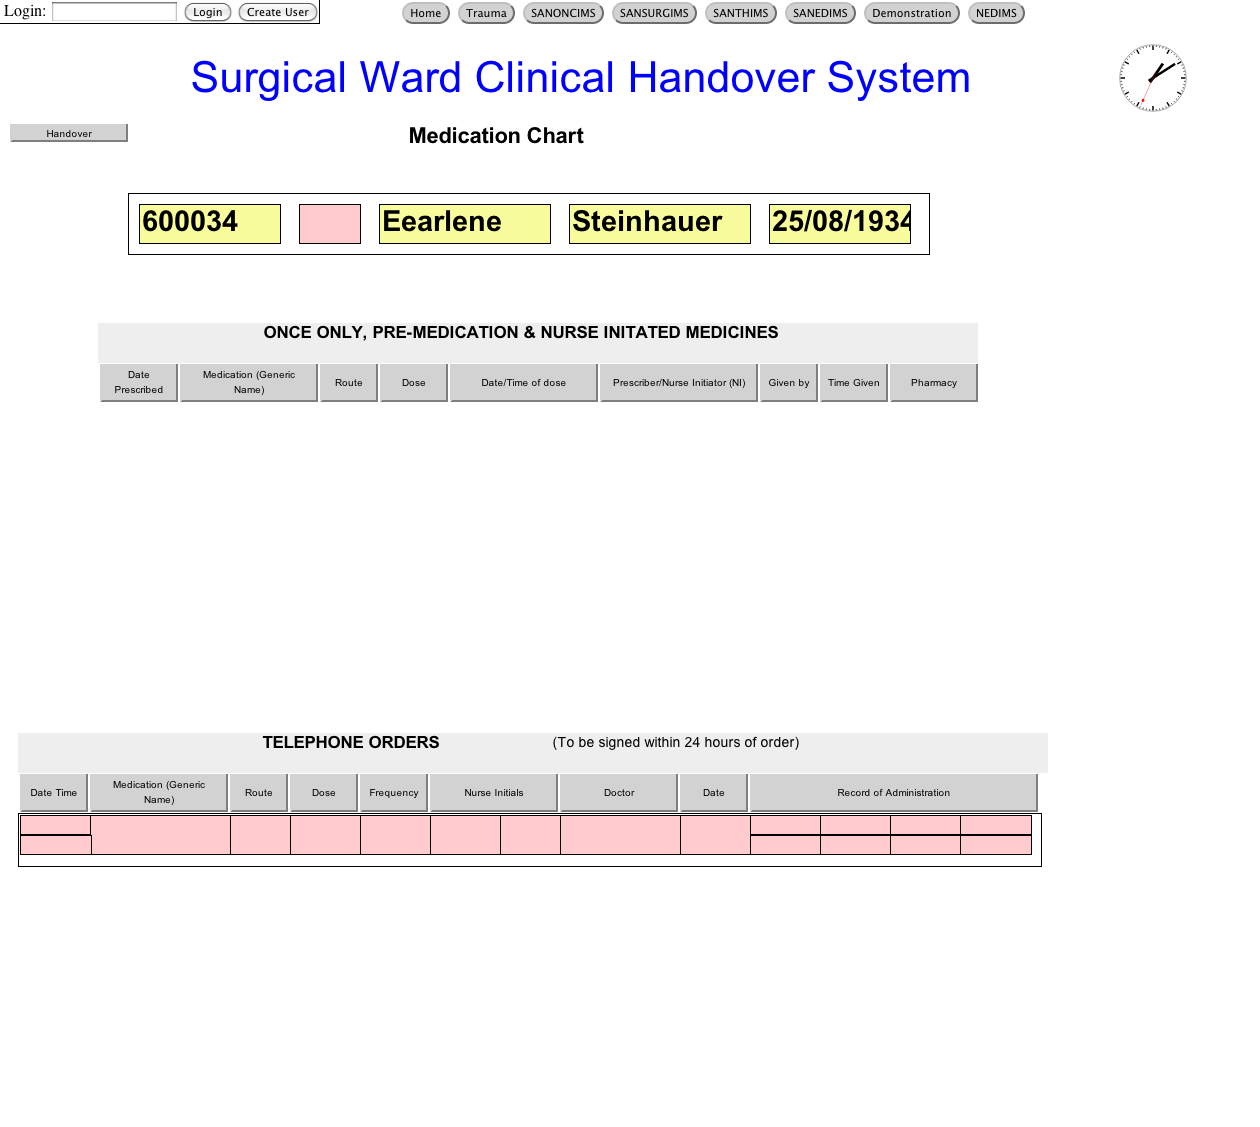
\includegraphics[scale=1.0, width=180mm]{Images/iCIMS-MedicationChart}
				\caption{Medication Chart Form}
\end{figure}

\newpage
\subsubsection{Temporary Transfer/Handover Ticket To Ride Form}
\label{Temporary Transfer/Handover Ticket To Ride Form}

\begin{figure}[hp]
				\centering
				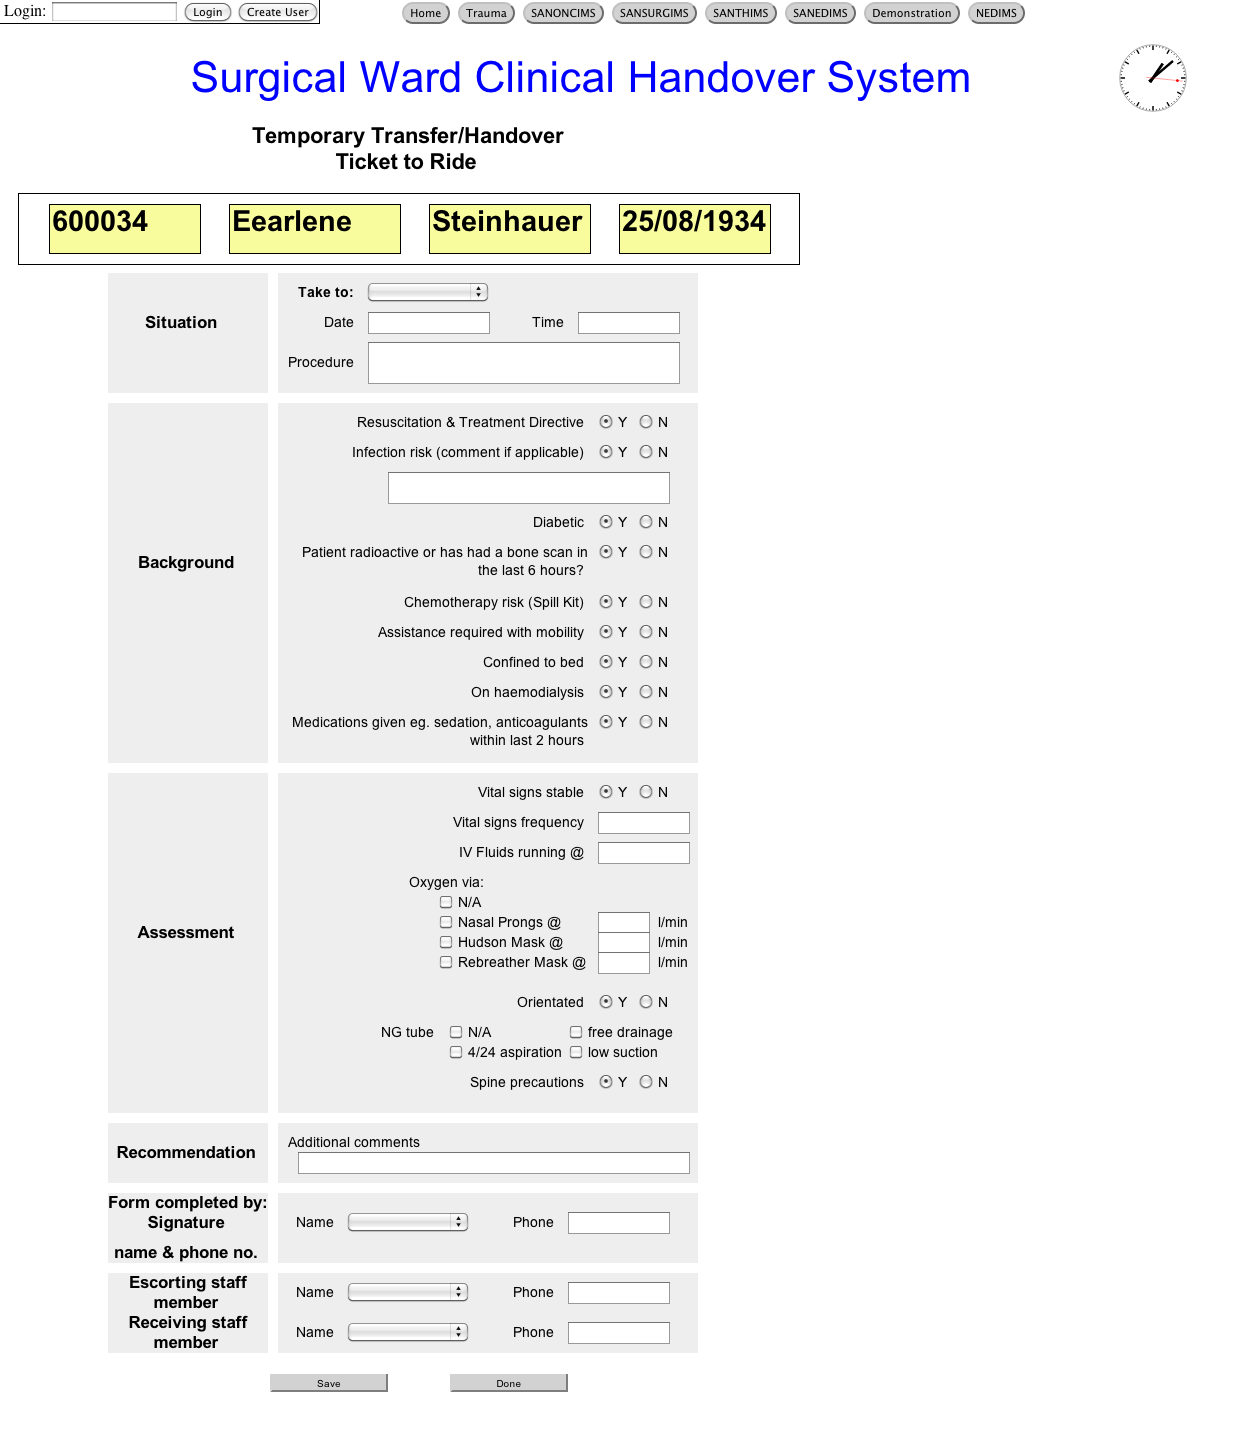
\includegraphics[scale=1.0, width=140mm]{Images/iCIMS-TempTransHandoverTicketToRide}
				\caption{Temporary Transfer/Handover Ticket To Ride Form}
\end{figure}
